\documentclass[10pt,twoside]{article}

\usepackage{iftex}

\ifPDFTeX
\usepackage[utf8]{inputenc}
\usepackage[T1]{fontenc}
\usepackage{mathptmx}
\usepackage[scaled=0.92]{helvet}
\newcommand{\arialfont}{\fontfamily{phv}\selectfont}
\else
\usepackage{fontspec}
\defaultfontfeatures{Ligatures=TeX}

\IfFontExistsTF{Times New Roman}
{\setmainfont{Times New Roman}}
{\setmainfont{TeX Gyre Termes}}

\IfFontExistsTF{Arial}
{\setsansfont{Arial}\newfontfamily\arialfont{Arial}}
{\setsansfont{TeX Gyre Heros}\newfontfamily\arialfont{TeX Gyre Heros}}
\fi

% ------------------ Page layout for the FAIR template ------------------
\usepackage[
paperwidth=20.5cm,
paperheight=29.5cm,
top=2.2cm,
bottom=1.8cm,
left=1.8cm,
right=1.8cm,
headheight=11.4pt,
headsep=0.4cm,
footskip=0.8cm
]{geometry}

% ------------------ Packages ------------------
\usepackage{amsmath,amssymb}
\usepackage{graphicx}
\usepackage{array}
\usepackage{longtable}
\usepackage{caption}
\usepackage{subcaption}
\usepackage{float}
\usepackage{enumitem}
\usepackage{fancyhdr}
\usepackage{titlesec}
\usepackage{indentfirst}
\usepackage{url}
\IfFileExists{cite.sty}{\usepackage{cite}}{}

\newcommand{\fairsmallfont}{\fontsize{9pt}{11pt}\selectfont}
\newcommand{\fairbodyfont}{\fontsize{10pt}{12pt}\selectfont}

\newlength{\fairfigurewidth}
\setlength{\fairfigurewidth}{12cm}

\newcommand{\xairesultcell}[3][\linewidth]{%
  \begin{minipage}[c]{\linewidth}
    \centering
    {\fairsmallfont #2\par}
    \includegraphics[width=#1]{#3}
  \end{minipage}%
}

\newcommand{\modelcurvecell}[2]{%
  \begin{minipage}[c]{\linewidth}
    \centering
    \vspace{2pt}%
    \textbf{#1}\par
    \vspace{1pt}%
    \includegraphics[width=\linewidth]{#2}
    \vspace{1pt}%
  \end{minipage}%
}

% ------------------ Paragraph style ------------------
\setlength{\parindent}{1cm}
\setlength{\parskip}{6pt}
\emergencystretch=2em
\raggedbottom

% ------------------ Paper metadata ------------------
\newcommand{\fairsuperscript}[1]{%
  \raisebox{0.8ex}{\fontsize{8pt}{8pt}\selectfont #1}%
}
\newcommand{\PaperTitle}{CORPORATE CREDIT RATING BASED ON MACHINE LEARNING MODELS}
\newcommand{\PaperShortTitle}{CORPORATE CREDIT RATING BASED ON MACHINE LEARNING MODELS}
\newcommand{\PaperAuthors}{Le Nguyen Thanh Tai\fairsuperscript{1}}
\newcommand{\PaperShortAuthors}{Le Nguyen Thanh Tai}
\newcommand{\PaperAffiliations}{%
\fairsuperscript{1}Faculty of Information Technology, Vinh Long University of Technology Education
}
\newcommand{\PaperEmail}{22022001@st.vlute.edu.vn}
\newcommand{\FairConference}{}

% ------------------ Header/Footer ------------------
\pagestyle{fancy}
\fancyhf{}

% Even pages: page number on the left, short title on the right.
% Odd pages: short author name on the left, page number on the right.
\fancyhead[LE,RO]{\fairsmallfont\thepage}
\fancyhead[RE]{\fairsmallfont\PaperShortTitle}
\fancyhead[LO]{\fairsmallfont\PaperShortAuthors}

% The template uses a thin rule below the header on subsequent pages.
\renewcommand{\headrulewidth}{0.4pt}
\renewcommand{\footrulewidth}{0pt}

\fancypagestyle{firstpage}{%
\fancyhf{}%
\fancyhead[C]{\fairsmallfont\FairConference}%
\renewcommand{\headrulewidth}{0.4pt}
}

% ------------------ Title block ------------------
\newcommand{\makefairtitle}{%
\thispagestyle{firstpage}%
\begin{center}
{\arialfont\bfseries\fontsize{14pt}{16pt}\selectfont\MakeUppercase{\PaperTitle}\par}
\vspace{3pt}
{\bfseries\fontsize{12pt}{14pt}\selectfont\PaperAuthors\par}
\vspace{3pt}
{\fairsmallfont\PaperAffiliations\par}
\vspace{3pt}
{\itshape\fairsmallfont\PaperEmail\par}
\end{center}
\vspace{6pt}%
}

% ------------------ Abstract / Keywords ------------------
\newcommand{\FairDash}{\unskip\textemdash\space}

\newenvironment{fairabstract}{%
\begingroup
\fairsmallfont
\itshape
\setlength{\parindent}{1cm}%
\setlength{\parskip}{6pt}%
}{%
\par\endgroup
}

\newcommand{\fairabstracttext}[1]{%
\begin{fairabstract}
\textbf{ABSTRACT}\FairDash #1
\end{fairabstract}
}

\newcommand{\fairkeywords}[1]{%
\begin{fairabstract}
\textbf{Keywords}\FairDash #1
\end{fairabstract}
}

% ------------------ Section numbering ------------------
\setcounter{secnumdepth}{4}

\renewcommand{\thesection}{\Roman{section}}
\renewcommand{\thesubsection}{\Alph{subsection}}
\renewcommand{\thesubsubsection}{\arabic{subsubsection}}
\renewcommand{\theparagraph}{\alph{paragraph}}

\titleformat{\section}
{\centering\fairsmallfont\bfseries}
{\thesection.}{0.5em}{}

\titleformat{\subsection}
{\fairsmallfont\bfseries\itshape}
{\thesubsection.}{0.5em}{}

\titleformat{\subsubsection}
{\fairsmallfont\bfseries\itshape}
{\thesubsubsection.}{0.5em}{}

\titleformat{\paragraph}[block]
{\normalsize}
{\theparagraph.}{0.5em}{}

\titlespacing*{\section}{0pt}{6pt}{6pt}
\titlespacing*{\subsection}{0pt}{6pt}{3pt}
\titlespacing*{\subsubsection}{0pt}{6pt}{3pt}
\titlespacing*{\paragraph}{0pt}{6pt}{3pt}

% ------------------ Figure/Table captions ------------------
\renewcommand{\figurename}{Figure}
\renewcommand{\tablename}{Table}

\captionsetup{
font=normalsize,
labelsep=period,
justification=centering,
singlelinecheck=true,
skip=5pt
}

\setlength{\intextsep}{5pt}
\newcommand{\setupfairsubfigures}{%
  \captionsetup[subfigure]{%
    labelformat=simple,
    labelsep=period,
    font=it,
    justification=centering
  }%
  \renewcommand{\thesubfigure}{\alph{subfigure}}%
}

% ------------------ Lists ------------------
\setlist[itemize]{
leftmargin=1.27cm,
itemsep=0pt,
topsep=0pt,
parsep=0pt
}

% ------------------ Bibliography ------------------
\makeatletter
\renewenvironment{thebibliography}[1]{%
\section*{REFERENCES}%
\fairbodyfont
\hbadness=10000
\setlength{\parskip}{0pt}%
\list{[\arabic{enumiv}]}{%
\settowidth\labelwidth{[#1]}%
\leftmargin\labelwidth
\advance\leftmargin\labelsep
\usecounter{enumiv}%
\let\p@enumiv\@empty
\renewcommand{\theenumiv}{\arabic{enumiv}}%
}%
\sloppy
\clubpenalty4000
\widowpenalty4000
}{%
\endlist
}
\makeatother

\urlstyle{same}

% =========================================================
% DOCUMENT
% =========================================================
\begin{document}

\makefairtitle

\fairabstracttext{%
Corporate credit rating supports the assessment of financial health, debt-servicing capacity, and early warning of credit risk. This study develops a credit rating system based on financial data and compares LightGBM, XGBoost, LSTM, TCN, PatchTST, Transformer-LSTM, and GraphSAGE models. The experimental dataset consists of 8,680 observations from 1,623 firms during the period 2005--2016. Each observation is represented by 12 financial ratios covering liquidity, leverage, profitability, operating efficiency, and cash flow, and is classified into three groups: Distressed, High Yield, and Investment Grade. In addition to individual models, the study implements Fuzzy Choquet Integral and Gompertz Fuzzy Ranking ensembles and proposes a Dynamic Model Fusion mechanism that combines Transformer-LSTM with GraphSAGE. When the two component models produce different predictions, the Dynamic Classifier Selection mechanism selects a model based on its validation-set competence and sample-level confidence. Dynamic Model Fusion achieves the best overall performance on the test set, with an Accuracy of 92.98\%, Precision of 92.67\%, Recall of 92.98\%, and F1-score of 92.60\%. GradientSHAP and LIME are used to analyze the influence of financial features. The explanation results indicate the substantial roles of profit margins, the debt-to-equity ratio, and liquidity, thereby supporting the interpretation of the system's classification decisions.
}

\fairkeywords{%
Corporate credit rating, Machine learning, Deep learning, Ensemble learning, Explainable artificial intelligence.
}

\section{INTRODUCTION}
\subsection{Problem introduction}
Corporate credit rating reflects a firm's repayment capacity, risk level, and financial health. In the context of fluctuating interest rates and capital markets, default-risk assessment is important for banks, investors, and regulatory authorities. According to S\&P Global Ratings, 117 global defaults were recorded in 2025, with the total amount of defaulted debt exceeding USD 140 billion \cite{noauthor_default_nodate}. The local-currency bond market in emerging East Asia reached approximately USD 29.5 trillion by the end of 2025 \cite{bank_asia_2025}. In Vietnam, the corporate bond market reached approximately VND 1.42 quadrillion, equivalent to nearly 11\% of GDP; new issuance in 2025 increased by 32\% and exceeded VND 624 trillion \cite{noauthor_tong_nodate}. These figures highlight the need for credit assessment methods that are verifiable and interpretable. Financial data often fluctuate, while the relationship between financial ratios and credit risk may be nonlinear. Traditional assessment methods depend heavily on expert judgment; in contrast, machine learning models may be difficult to interpret when used as ``black-box'' systems. Therefore, this study develops and compares machine learning, deep learning, and graph-based models for credit-risk classification, while using XAI to analyze the roles of financial ratios in prediction.

\subsection{Related studies}
Truong Thi Thuy Duong and Le Hai Trung \cite{thuy_ung_2023} evaluated six algorithms on 300 Vietnamese firms during 2017--2019, where XGBoost achieved an Accuracy of 87.73\%, higher than Random Forest at 83.49\%. On a larger dataset, Andersson \cite{andersson_machine_2023} reported that Gradient Boosting achieved an Accuracy of approximately 90\% in predicting ratings issued by Standard \& Poor's, Moody's, and Fitch. Deep learning architectures extend the ability to exploit temporal dependencies and multimodal information. Kofune et al. \cite{kofune_enhancing_2026} proposed Transformer-LSTM and achieved an Accuracy of 89.96\%. Chen and Long \cite{chen_novel_2020} used Self-Attention in the SMAGRU model, obtaining an Accuracy of 93.33\%. Morthens \cite{morthens_1989-_credit_2024} combined sequential and graph models to exploit temporal financial data and corporate relationships; GRU and GRU-GCNGRU achieved 75.25\% and 74.44\%, respectively. Fang et al. \cite{fang_design_2025} combined feature selection, oversampling, and CNN-BiLSTM-AM on financial text data, achieving an Accuracy of 88\%. For graph-based approaches, Feng et al. \cite{feng_every_2020} proposed CCR-GNN for corporate credit rating and reported an Accuracy of 95\% on listed Chinese companies. A subsequent study developed HHGNN to exploit hierarchical structure, heterogeneity, and unlabeled data in corporate networks, achieving an Accuracy of 97.557\% \cite{feng_corporate_2024}. Liu and Kok \cite{liu_prediction_2025} used a Heterogeneous Topological Graph Neural Network for bank credit-rating prediction and achieved an Accuracy of 70.57\%. These results indicate that the effectiveness of each architecture depends considerably on the data source and evaluation protocol. The present study therefore evaluates tree-based models, sequential models, and graph-based models under a unified setting on the same dataset, while examining dynamic fusion and prediction explainability.

\section{RELATED WORK}

\subsection{Characteristics of corporate credit rating}

Corporate credit rating evaluates a firm's financial credibility and ability to meet debt obligations over a specified period \cite{phu_nghi_nodate}. Rating results support banks, investors, and regulatory authorities in credit granting, bond investment, and risk monitoring \cite{hai_mo_2023}. Firms with strong profitability, stable cash flow, and low leverage generally belong to better credit groups, whereas firms with weak cash flow, high debt levels, or potential insolvency belong to higher-risk groups \cite{thuy_ung_2023}. This study divides ratings into three groups: Investment Grade (IG), High Yield (HY), and Distressed. IG indicates low risk; HY represents a higher level of risk; and Distressed denotes weak financial conditions and a high probability of default \cite{hung_xep_2023}. The relationships between liquidity, leverage, profitability, cash-flow indicators, and credit risk are often nonlinear and time-varying \cite{hai_mo_2023}. Therefore, this study combines machine learning, deep learning, and Explainable Artificial Intelligence (XAI) to evaluate classification performance and support the interpretation of financial indicators \cite{gramegna_shap_2021}.

\subsection{Machine learning models used in training}

\subsubsection{LightGBM model (Light Gradient Boosting Machine)}
LightGBM (Light Gradient Boosting Machine) is an ensemble learning algorithm in the Gradient Boosting Decision Tree (GBDT) family \cite{ke_lightgbm_2017}. The algorithm uses a leaf-wise tree growth strategy along with sampling and feature-bundling techniques to reduce computational and memory costs on high-dimensional data.

\subsubsection{XGBoost model (eXtreme Gradient Boosting)}
XGBoost (eXtreme Gradient Boosting) is a scalable implementation of GBDT that combines a regularized objective function with computational optimization techniques \cite{chen_xgboost_2016}. This mechanism helps control model complexity and efficiently handles tabular data.

\subsubsection{Temporal Convolutional Network (TCN)}
A Temporal Convolutional Network (TCN) uses causal convolutions and dilated convolutions to process sequential data \cite{bai_empirical_2018}. Compared with recurrent architectures, TCN enables parallel computation and expands the receptive field without violating temporal order.

\subsubsection{Long Short-Term Memory network (LSTM)}
Long Short-Term Memory (LSTM) is a variant of recurrent neural networks that uses memory states and gating mechanisms to reduce the effect of vanishing gradients \cite{hochreiter_long_1997}. As a result, LSTM can learn long-term dependencies in sequential data.

\subsubsection{PatchTST architecture (Patch Time Series Transformer)}
PatchTST divides a time series into subsequences, or patches, and uses a Transformer to learn representations among these patches \cite{nie_time_2023}. This representation reduces the input sequence length and helps the model capture both local structure and long-term dependencies.

\subsubsection{Hybrid T-LSTM model (Transformer-Long Short-Term Memory)}
The hybrid T-LSTM model (Transformer-Long Short-Term Memory) \cite{kofune_enhancing_2026} combines Transformer and LSTM components to effectively exploit time-series financial data. In corporate credit rating, financial data not only reflect a firm's condition at a given point in time but also capture changes across consecutive periods. Therefore, T-LSTM is used to learn both long-range relationships and sequential dependencies in financial-ratio sequences.

\subsubsection{GraphSAGE graph neural network (Graph Sample and Aggregate)}
GraphSAGE is an inductive node representation learning framework in which each node representation is formed by aggregating the features of the node itself and its neighboring nodes \cite{hamilton_inductive_2018}. Unlike methods that learn a fixed vector for each node, GraphSAGE can generate representations for nodes that did not appear during training.

\subsubsection{Model evaluation metrics}
\paragraph{Accuracy}
Accuracy \cite{grandini_metrics_2020} is the ratio of correctly predicted samples to the total number of samples in the dataset. It is a simple and interpretable metric commonly used in classification tasks to evaluate overall model performance. Accuracy is computed as follows:
\begin{equation} Accuracy = \frac{TP + TN}{TP + TN + FP + FN}
\end{equation} where:
\begin{itemize}
\item $TP$ (True Positive): the number of positive samples correctly predicted as positive.
\item $TN$ (True Negative): the number of negative samples correctly predicted as negative.
\item $FP$ (False Positive): the number of negative samples incorrectly predicted as positive.
\item $FN$ (False Negative): the number of positive samples incorrectly predicted as negative.
\end{itemize}
\paragraph{Precision}
Precision \cite{grandini_metrics_2020} measures the proportion of correct positive predictions among all positive predictions. This metric is particularly important in applications where false positives may lead to serious consequences.
\begin{equation}
\mathrm{Precision}=\frac{TP}{TP+FP}
\end{equation}
\paragraph{Recall}
Recall \cite{grandini_metrics_2020} measures the proportion of correct positive predictions among all actual positive samples. Recall is important in situations where detecting all positive cases is necessary, even if this results in some negative cases being predicted as positive.
\begin{equation}
\mathrm{Recall}=\frac{TP}{TP+FN}
\end{equation}
\paragraph{F1-score}
The F1-score \cite{grandini_metrics_2020} is the harmonic mean of Precision and Recall. It balances the correctness of positive predictions and the ability to detect positive samples.
\begin{equation}
F1=2\times\frac{\mathrm{Precision}\times\mathrm{Recall}}{\mathrm{Precision}+\mathrm{Recall}}
\end{equation}
\paragraph{AUC-ROC}
The ROC curve represents the relationship between the True Positive Rate (Recall) and the False Positive Rate. AUC is the area under the ROC curve and indicates the model's ability to distinguish between classes \cite{fawcett_introduction_2006}. A model with an AUC close to 1 is considered strong, whereas an AUC close to 0.5 indicates near-random performance.
\begin{equation}
\mathrm{TPR}=\frac{TP}{TP+FN}\quad;\quad \mathrm{FPR}=\frac{FP}{FP+TN}
\end{equation}

\subsection{Ensemble learning methods}
\subsubsection{Fuzzy Choquet Integral}
Fuzzy Choquet Integral is an ensemble learning method based on fuzzy measures and is used to aggregate prediction outputs from multiple component models. Unlike weighted averaging, this method considers not only the individual importance of each model but also the interactions among models in the ensemble \cite{zadeh_fuzzy_1965, choquet_theory_1954}. Let $x_1, x_2, \ldots, x_n$ denote the prediction probabilities of $n$ models sorted in ascending order, $x_{(1)} \leq x_{(2)} \leq \cdots \leq x_{(n)}$. The discrete Choquet integral is computed as follows:
\begin{equation} C_{\mu}(x) = \sum_{i=1}^{n} \left(x_{(i)} - x_{(i-1)}\right)\mu(A_{(i)}), \end{equation}
where $x_{(0)}=0$, $A_{(i)}=\{(i),(i+1),\ldots,(n)\}$, and $\mu(A_{(i)})$ is a fuzzy measure representing the importance of the corresponding set of models.

\subsubsection{Gompertz Fuzzy Ranking}
Gompertz Fuzzy Ranking is an ensemble learning method that uses the Gompertz function to assign fuzzy weights to component models based on the ranks of their predicted probabilities. This idea is adapted from the study by Kundu et al. \cite{kundu_fuzzy_2021}, where the Gompertz function was used to fuse the outputs of multiple CNN models for COVID-19 CT image screening. In this study, however, the method is transferred and adapted to corporate credit rating. Therefore, the citation \cite{kundu_fuzzy_2021} is used as the methodological basis for fuzzy rank-based fusion, rather than as direct empirical evidence in the credit-rating domain. Unlike ordinary probability averaging, Gompertz Fuzzy Ranking prioritizes models with more confident predictions through probability ranking while reducing the influence of models with low prediction probabilities. Let $p_i^{(c)}$ be the predicted probability of the $i$-th model for class $c$. These probabilities are ranked as $r_i$, where a model with a higher probability receives a better rank. The Gompertz fuzzy weight is defined as follows:
\begin{equation}
w_i = \frac{\exp \left(-\alpha e^{-\beta r_i}\right)} {\sum_{j=1}^{M} \exp \left(-\alpha e^{-\beta r_j}\right)}
\end{equation}
where $M$ is the number of component models, and $\alpha$ and $\beta$ are parameters controlling the slope of the Gompertz function. The fused prediction score for class $c$ is computed as:
\begin{equation}
S_c = \sum_{i=1}^{M} w_i p_i^{(c)}
\end{equation}
The final predicted label is determined by the class with the highest fused score. In corporate credit rating, Gompertz Fuzzy Ranking adjusts the contribution of component models according to the relative confidence of each prediction, making the fusion result more flexible than fixed voting or averaging methods.

\subsubsection{Dynamic Model Fusion}
Dynamic Model Fusion (DMF) is a dynamic model-combination method in which the final output is selected based on each model's confidence for each data sample. This idea is adapted from the study by Toufiq and Pal \cite{toufiq_explainable_2026}, where a dynamic fusion mechanism was used to combine GCNN and CNN for brain tumor analysis from MRI images. In this study, however, the method is transferred and adapted to corporate credit rating. Therefore, the citation \cite{toufiq_explainable_2026} is used as the methodological basis for Dynamic Model Fusion and Dynamic Classifier Selection, rather than as direct empirical evidence in the credit-rating domain. In this study, DMF combines T-LSTM and GraphSAGE. T-LSTM is advantageous for exploiting temporal financial trends, whereas GraphSAGE supports learning graph relationships among firms. Let $\hat{y}_{T}$ and $\hat{y}_{G}$ denote the predicted labels of T-LSTM and GraphSAGE, respectively. If the two models produce the same label, the final result is defined as follows:
\begin{equation} \hat{y} = \hat{y}_{T} = \hat{y}_{G} \end{equation}
Conversely, if the two models produce different predictions, the system calculates a dynamic confidence score for each model based on its validation-set competence and the prediction probability for the test sample:
\begin{equation} R_m(x) = \lambda V_m(\hat{y}_m) + (1-\lambda) P_m(\hat{y}_m|x), \end{equation}
where $R_m(x)$ is the confidence score of model $m$, $V_m(\hat{y}_m)$ is the model's validation-set competence for the predicted class, $P_m(\hat{y}_m|x)$ is the model's predicted probability for sample $x$, and $\lambda$ is a balancing coefficient. The final label is selected from the model with the higher confidence score:
\begin{equation} \hat{y} = \hat{y}_{\arg\max_m R_m(x)} \end{equation}
This mechanism enables the system to take advantage of the strengths of both sequential and graph-based models while avoiding the use of fixed weights for all samples.

\subsection{Explainable artificial intelligence methods}
\subsubsection{GradientSHAP}
GradientSHAP is a gradient-based explanation method that combines the idea of SHAP with random sampling between the sample to be explained and background samples. The method estimates each feature's contribution by computing the gradient of the model output with respect to the input at multiple interpolated points between the explained sample and baseline samples \cite{lundberg_unified_2017, kokhlikyan_captum_2020}.

\subsubsection{LIME}
LIME is a local, model-agnostic explanation method proposed by Ribeiro et al. to explain a specific prediction using a simple model in the neighborhood of the sample being analyzed \cite{ribeiro_why_2016}. The main idea of LIME is to generate multiple perturbed samples around the original observation, feed these samples into the model to obtain prediction probabilities, and then train a weighted local linear model to approximate the behavior of the original model.

\section{PROPOSED METHOD}

This study proposes a two-phase system consisting of training and testing. The overall workflow is presented in Figure~\ref{fig:proposed_model}.
\begin{figure}[H]
    \centering
    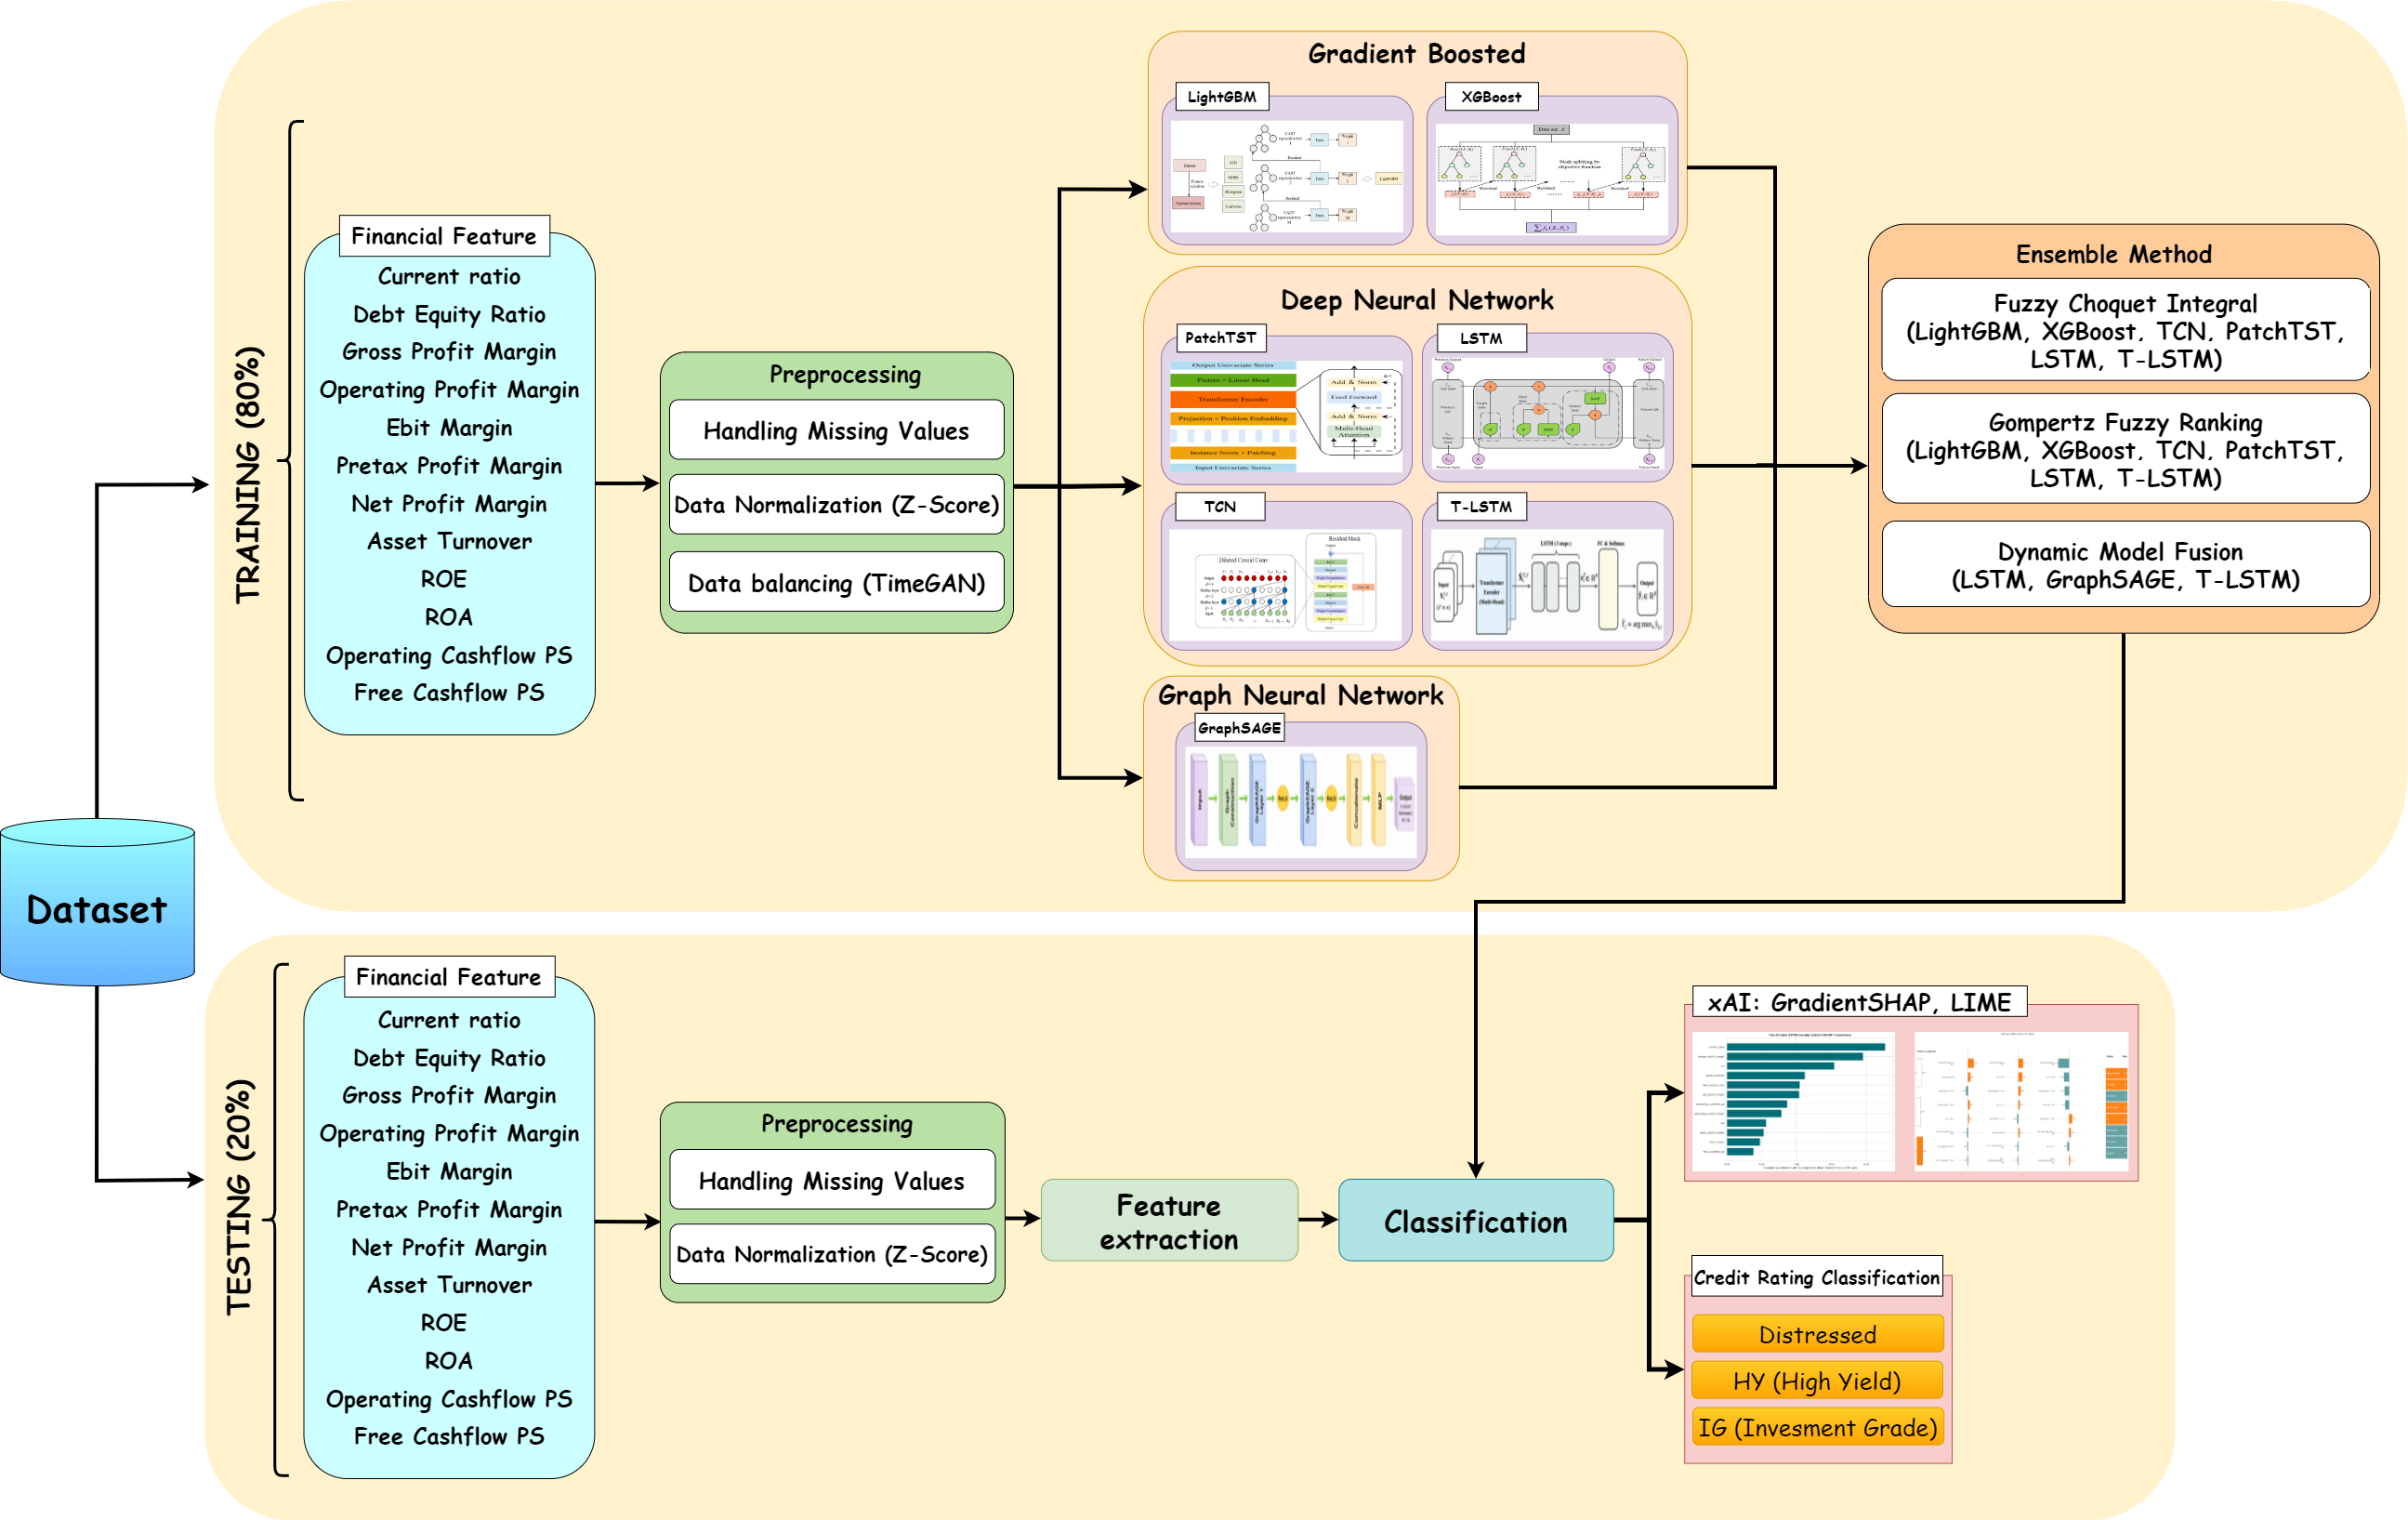
\includegraphics[width=\textwidth]{acc-loss/diagram_pipeline_overview.png}
    \caption{Proposed model}
    \label{fig:proposed_model}
\end{figure}

\subsection{Training phase}
\subsubsection{Data preprocessing and data preparation}
During the training phase, duplicate records based on ticker symbols and rating dates are merged. Median values are used for financial ratios, while rating labels are selected according to the higher-risk category to maintain a conservative principle. Missing values are imputed using medians estimated from the training set in order to reduce the influence of outliers and avoid data leakage. Skewed features are log-transformed when their skewness exceeds a predefined threshold. The 12 financial ratios are then standardized using Z-score normalization to reduce the effect of differences in scale. The original 21 credit-rating grades are grouped into three categories: Investment Grade (IG), High Yield (HY), and Distressed, thereby reducing label sparsity while preserving the risk order. The data are sorted by firm and time to create fixed-length sequence windows. TimeGAN is used to generate additional financial sequences for minority classes in the training set, thereby reducing class imbalance.

\subsubsection{Feature extraction and training}
Deep learning models extract sequential features directly from time windows. The input consists of standardized financial ratios, incremental features, and embedded categorical variables. Training uses AdamW and the cross-entropy loss function. Gradient clipping is applied to control gradients, while the F1-score is used to monitor convergence. The models are trained independently using the same preprocessing pipeline; loss and Accuracy are recorded for evaluation.

\subsection{Testing phase}
After training, the models are evaluated on a test set that has not appeared during training. Deep learning models are switched to evaluation mode using \texttt{eval()} to disable Dropout and fix the behavior of normalization layers. The outputs include predictions for the three groups IG, HY, and Distressed; performance is evaluated using Accuracy, Precision, Recall, F1-score, AUC-ROC, loss, and confusion matrices. Ensemble scenarios include TTX (TCN, T-LSTM, XGBoost), PLL (PatchTST, LSTM, LightGBM), and TTLPXL (T-LSTM, TCN, LSTM, PatchTST, XGBoost, LightGBM). The probabilities from component models are aggregated using Fuzzy Choquet Integral or Gompertz Fuzzy Ranking. The DMF scenario combines T-LSTM and GraphSAGE; when the two models disagree, Dynamic Classifier Selection selects the prediction based on validation-set competence and test-sample probability. GradientSHAP and LIME are applied in the testing phase to support interpretability. GradientSHAP estimates the contribution of each financial ratio at a global level, whereas LIME locally explains individual predictions.

\section{EXPERIMENTAL RESULTS}

\subsection{Experimental environment and dataset}

\subsubsection{Experimental environment}
The experiments are conducted on Kaggle Notebooks \cite{noauthor_notebooks_nodate}, using an Intel Xeon 2.00 GHz CPU with 4 vCPUs, 32 GB RAM, and an NVIDIA Tesla P100 GPU with 16 GB VRAM. The models are implemented using Python 3.8+ and PyTorch. Pandas and NumPy are used for data processing, while Matplotlib and Scikit-learn support visualization and evaluation. Kaggle's GPU time limit is considered when selecting batch size and memory configuration.

\subsubsection{Experimental dataset}
The dataset is compiled from two public Kaggle sources: \textit{Corporate Credit Rating} \cite{noauthor_corporate_credit_rating_nodate} and \textit{Corporate Credit Rating with Financial Ratios} \cite{noauthor_corporate_financial_ratios_nodate}. The two sources are linked by company name, ticker symbol, rating agency, and rating date. After cleaning, merging, and removing duplicate records, the dataset contains 8,680 observations from 1,623 firms during 2005--2016. Each observation includes 12 financial ratios: Current Ratio, Debt-to-Equity Ratio, Gross Profit Margin, Operating Profit Margin, EBIT Margin, Pretax Profit Margin, Net Profit Margin, ROE, ROA, Asset Turnover, Operating Cash Flow per Share, and Free Cash Flow per Share. These ratios represent liquidity, leverage, profitability, operating efficiency, and cash flow. The original 21 credit-rating grades are grouped into three categories: IG, HY, and Distressed. Each firm has approximately 5.35 ratings on average; therefore, the data contain both tabular structure and temporal information. To reduce data leakage across firms, the training, validation, and test sets are split independently by ticker symbol. The class distribution after label grouping is presented in Table~\ref{tab:class_distribution}.
\begingroup
\centering
\begin{longtable}{lccc}
\caption{Detailed number of samples in each original class}
\label{tab:class_distribution}\\
\hline
\textbf{Class} & \textbf{Train} & \textbf{Val} & \textbf{Test} \\
\hline
\endfirsthead
\caption[]{Detailed number of samples in each original class (continued)}\\
\hline
\textbf{Class} & \textbf{Train} & \textbf{Val} & \textbf{Test} \\
\hline
\endhead
\hline
\multicolumn{4}{r}{\fairsmallfont Continued on the next page}\\
\endfoot
\hline
\endlastfoot
Investment Grade (IG) & 3898 & 557 & 1114 \\
High Yield (HY) & 1970 & 281 & 563 \\
Distressed & 208 & 30 & 59 \\
\end{longtable}
\endgroup

\subsection{Experimental scenarios}
Fourteen experimental scenarios are divided into two groups. The first group includes seven individual, hybrid, and graph-based models: LightGBM, XGBoost, TCN, LSTM, PatchTST, T-LSTM, and GraphSAGE. The second group includes seven ensemble learning scenarios using Fuzzy Choquet Integral (FI), Gompertz Fuzzy Ranking (FR), or Dynamic Model Fusion (DMF). The configuration of each scenario is shown in Table~\ref{tab:experimental_scenarios}.
\begingroup
\centering
\begin{longtable}{c l l >{\raggedright\arraybackslash}p{6.5cm}}
\caption{Experimental scenarios}
\label{tab:experimental_scenarios}\\
\hline
\textbf{Scenario} & \textbf{Scenario name} & \textbf{Fusion method} & \textbf{Models used} \\
\hline
\endfirsthead
\caption[]{Experimental scenarios (continued)}\\
\hline
\textbf{Scenario} & \textbf{Scenario name} & \textbf{Fusion method} & \textbf{Models used} \\
\hline
\endhead
\hline
\multicolumn{4}{r}{\fairsmallfont Continued on the next page}\\
\endfoot
\hline
\endlastfoot
1 & LightGBM & -- & LightGBM \\
2 & XGBoost & -- & XGBoost \\
3 & TCN & -- & Temporal Convolutional Networks (TCN) \\
4 & LSTM & -- & Long Short-Term Memory (LSTM) \\
5 & PatchTST & -- & Patch Time Series Transformer (PatchTST) \\
6 & T-LSTM & -- & Transformer--Long Short-Term Memory (T-LSTM) \\
7 & GraphSAGE & -- & GraphSAGE, Multilayer Perceptron (MLP) \\
8 & FI-TTX & Fuzzy Choquet Integral & TCN + T-LSTM + XGBoost \\
9 & FI-PLL & Fuzzy Choquet Integral & PatchTST + LSTM + LightGBM \\
10 & FI-TTLPXL & Fuzzy Choquet Integral & TCN + T-LSTM + LSTM + PatchTST + XGBoost + LightGBM \\
11 & FR-TTX & Gompertz Fuzzy Ranking & TCN + T-LSTM + XGBoost \\
12 & FR-PLL & Gompertz Fuzzy Ranking & PatchTST + LSTM + LightGBM \\
13 & FR-TTLPXL & Gompertz Fuzzy Ranking & TCN + T-LSTM + LSTM + PatchTST + XGBoost + LightGBM \\
14 & DMF & Dynamic Model Fusion & GraphSAGE + T-LSTM \\
\end{longtable}
\endgroup

\begingroup
\centering
\begin{longtable}{c c c l c}
\caption{Training parameters for the scenarios}
\label{tab:hyperparameter}\\
\hline
\textbf{Scenario} & \textbf{Learning rate} & \textbf{Epochs} & \textbf{Loss function} & \textbf{Number of classes} \\
\hline
\endfirsthead
\caption[]{Training parameters for the scenarios (continued)}\\
\hline
\textbf{Scenario} & \textbf{Learning rate} & \textbf{Epochs} & \textbf{Loss function} & \textbf{Number of classes} \\
\hline
\endhead
\hline
\multicolumn{5}{r}{\fairsmallfont Continued on the next page}\\
\endfoot
\hline
\endlastfoot
1 & 3e-2 & 100 & Cross Entropy & 3 \\
2 & 3e-2 & 100 & Cross Entropy & 3 \\
3 & 3e-4 & 100 & Cross Entropy & 3 \\
4 & 3e-4 & 100 & Cross Entropy & 3 \\
5 & 3e-4 & 100 & Cross Entropy & 3 \\
6 & 3e-4 & 100 & Cross Entropy & 3 \\
7 & 6e-4 & 100 & Cross Entropy & 3 \\
\end{longtable}
\endgroup

Table~\ref{tab:hyperparameter} presents the training parameters configured for each experimental scenario. For LightGBM and XGBoost, a learning rate of $3\times10^{-2}$ is used in the boosting mechanism to control the contribution of each decision tree to the overall model; the number of learning iterations corresponds to the number of boosting rounds. For deep learning models such as TCN, LSTM, PatchTST, and T-LSTM, a smaller learning rate of $3\times10^{-4}$ is selected to stabilize weight updates and reduce oscillations when processing financial time-series data. GraphSAGE uses the AdamW optimizer with a learning rate of $6\times10^{-4}$ to stabilize node representation learning on the graph. All scenarios use the Cross Entropy loss function for the three-class credit-rating classification problem: Distressed, HY, and IG.

\subsection{Training results}

\begingroup
\centering
\begin{longtable}{c l c c c c}
\caption{Summary of training results for the models (\%)}
\label{tab:training_results}\\
\hline
\textbf{Scenario} & \textbf{Training model} & \textbf{Train Loss} & \textbf{Val Loss} & \textbf{Train Acc} & \textbf{Val Acc} \\
\hline
\endfirsthead
\caption[]{Summary of training results for the models (\%) (continued)}\\
\hline
\textbf{Scenario} & \textbf{Training model} & \textbf{Train Loss} & \textbf{Val Loss} & \textbf{Train Acc} & \textbf{Val Acc} \\
\hline
\endhead
\hline
\multicolumn{6}{r}{\fairsmallfont Continued on the next page}\\
\endfoot
\hline
\endlastfoot
1 & LightGBM  & 0.123 & 0.266 & 94.0 & 92.0 \\
2 & XGBoost   & 0.177 & 0.267 & 94.0 & 92.4 \\
3 & TCN       & 0.248 & 0.276 & 92.7 & 92.3 \\
4 & LSTM      & 0.190 & 0.268 & 94.0 & 92.2 \\
5 & PatchTST  & 0.217 & 0.279 & 93.2 & 91.7 \\
6 & T-LSTM    & 0.167 & 0.223 & 94.0 & 92.4 \\
7 & GraphSAGE & 0.343 & 0.399 & 92.1 & 92.2 \\
\end{longtable}
\endgroup

\subsubsection{Accuracy}
\begin{figure}[H]
    \centering
    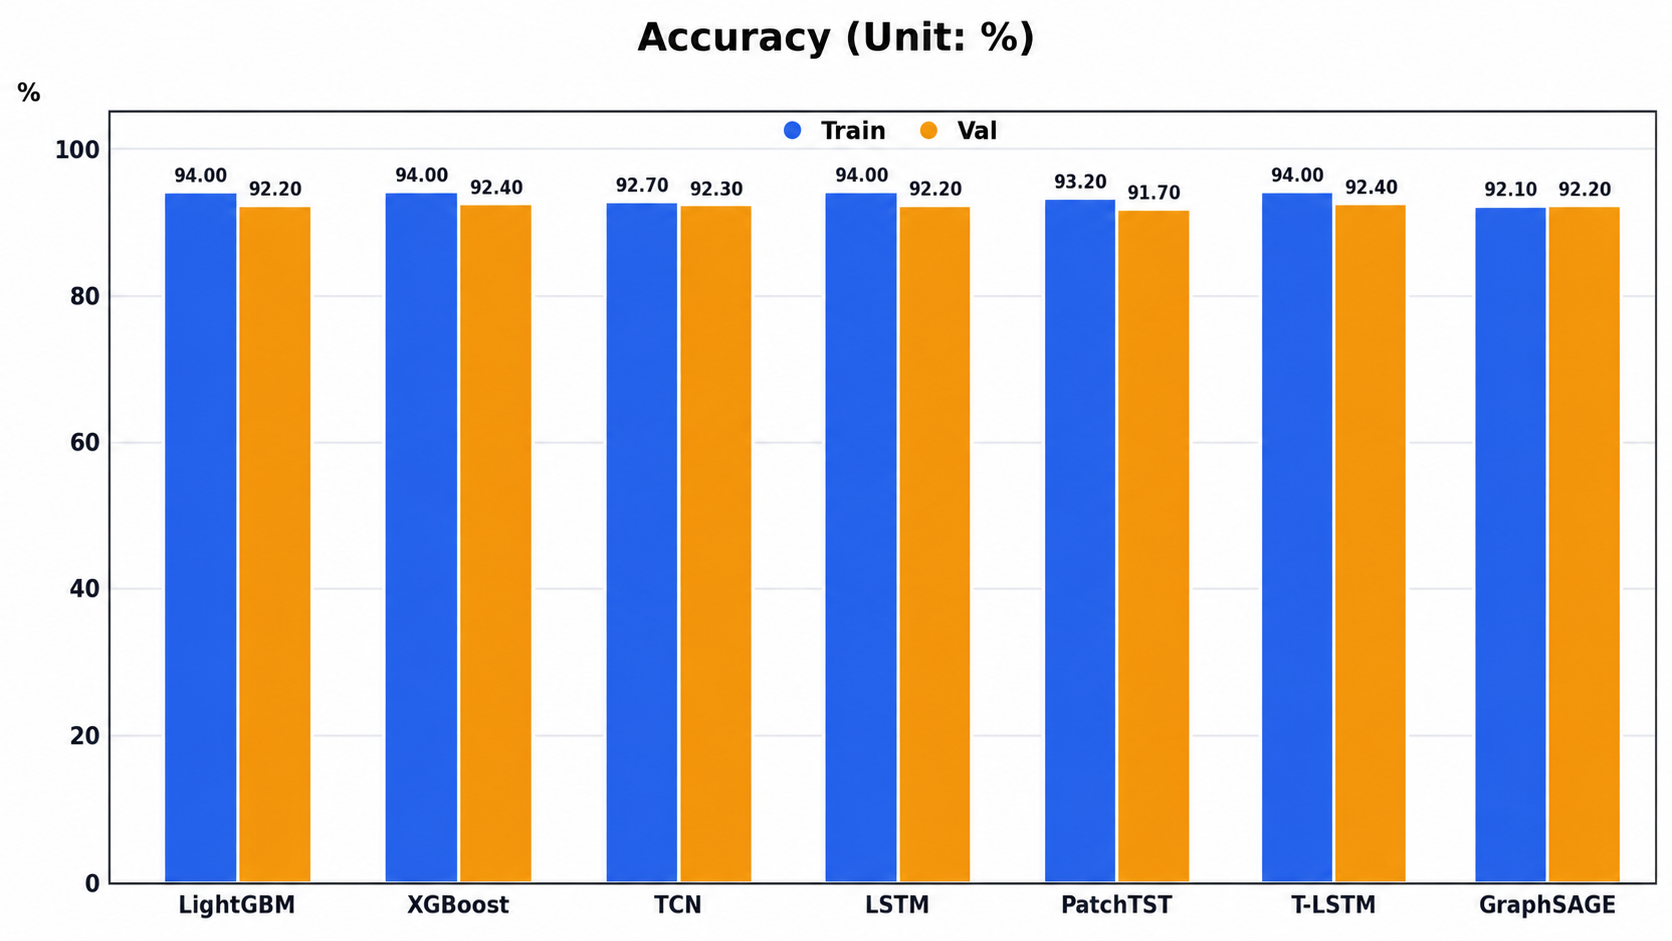
\includegraphics[width=\fairfigurewidth]{acc-loss/curve_accuracy_overall_english.png}
    \caption{Accuracy chart}
    \label{fig:acc-train}
\end{figure}

Figure~\ref{fig:acc-train} shows that training Accuracy ranges from 92.10\% to 94.00\%, whereas validation Accuracy ranges from 91.70\% to 92.40\%. XGBoost and T-LSTM both achieve the highest validation Accuracy, at 92.40\%. TCN and GraphSAGE show training-validation gaps of 0.40 and 0.10 percentage points, respectively. PatchTST obtains the lowest validation Accuracy, at 91.70\%. The range of 0.70 percentage points indicates that differences among the models on the validation set are relatively small. The training accuracy curves for the individual models are presented in detail in Table~\ref{tab:accuracy_models}.

\begingroup
\centering
\renewcommand{\arraystretch}{1.2}
\setlength{\tabcolsep}{2pt}
\begin{longtable}{>{\centering\arraybackslash}p{0.48\textwidth}|
                  >{\centering\arraybackslash}p{0.48\textwidth}}
\caption{Accuracy curves of the models}
\label{tab:accuracy_models}\\
\hline
\modelcurvecell{Scenario 1: LightGBM}{acc-loss/curve_accuracy_lightgbm.png} &
\modelcurvecell{Scenario 2: XGBoost}{acc-loss/curve_accuracy_xgboost.png} \\
\hline
\modelcurvecell{Scenario 3: TCN}{acc-loss/curve_accuracy_tcn.png} &
\modelcurvecell{Scenario 4: LSTM}{acc-loss/curve_accuracy_lstm.png} \\
\hline
\modelcurvecell{Scenario 5: PatchTST}{acc-loss/curve_accuracy_patchtst.png} &
\modelcurvecell{Scenario 6: T-LSTM}{acc-loss/curve_accuracy_tlstm.png} \\
\hline
\modelcurvecell{Scenario 7: GraphSAGE}{acc-loss/curve_accuracy_graphsage.png} & \\
\hline
\end{longtable}
\endgroup

\subsubsection{Loss}
\begin{figure}[H]
    \centering
    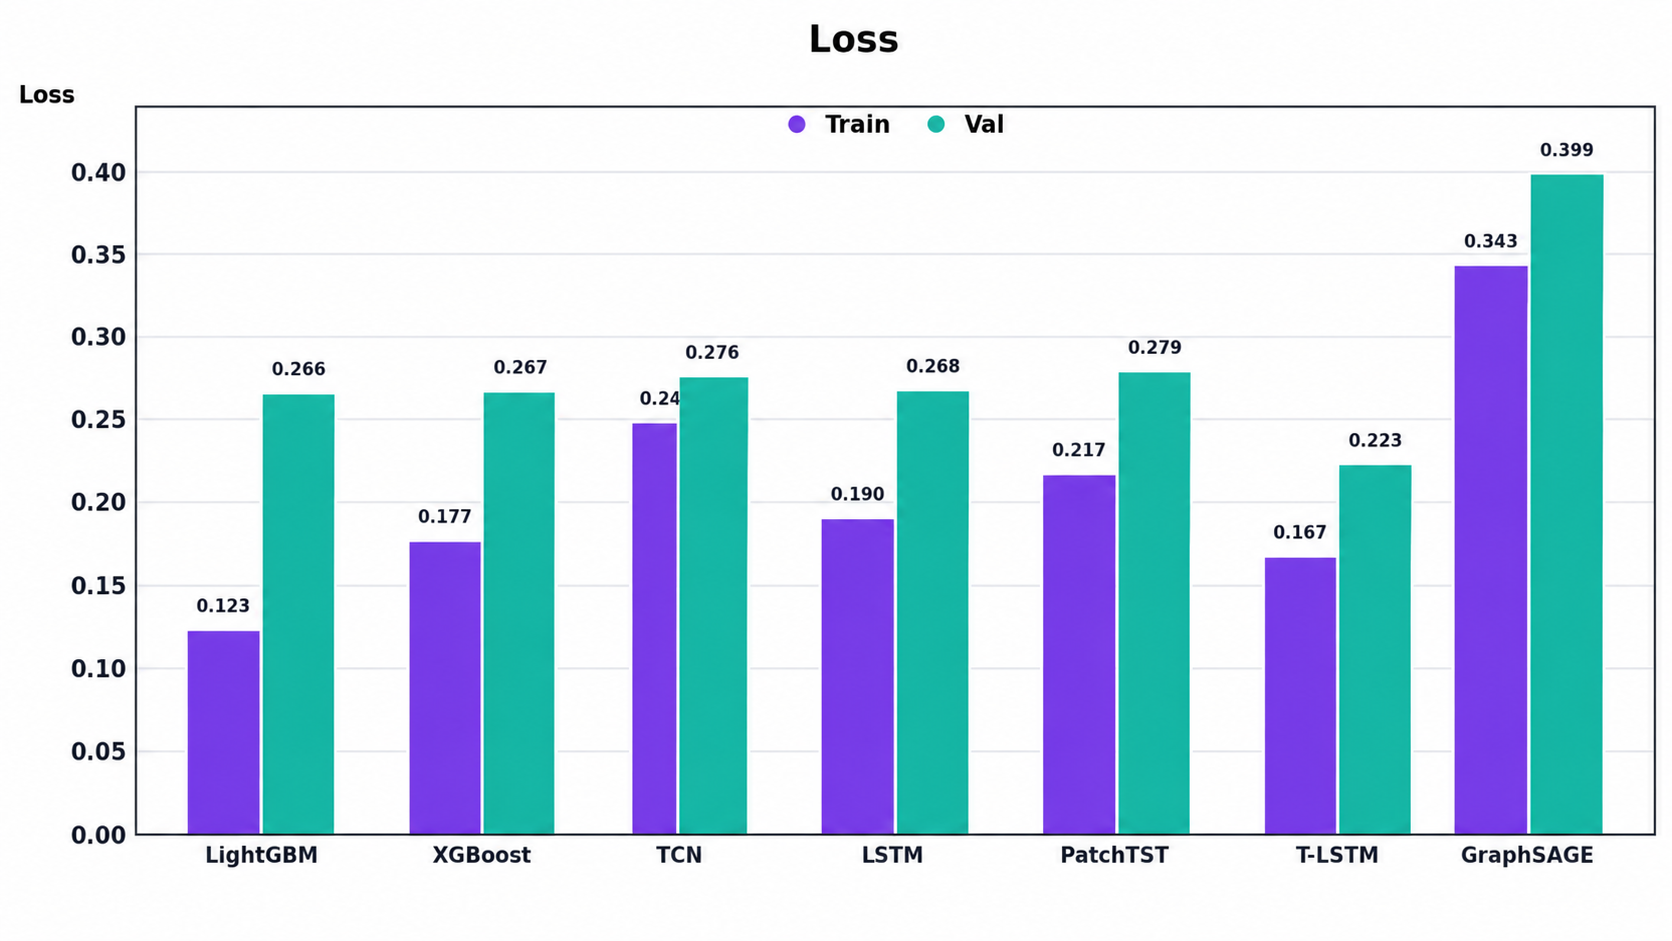
\includegraphics[width=\fairfigurewidth]{acc-loss/curve_loss_overall_english.png}
    \caption{Loss chart}
    \label{fig:loss-train}
\end{figure}

Figure~\ref{fig:loss-train} shows that training loss ranges from 0.123 to 0.343, while validation loss ranges from 0.223 to 0.399. T-LSTM obtains the lowest validation loss (0.223), followed by LightGBM (0.266), XGBoost (0.267), and LSTM (0.268). GraphSAGE records the highest values on both the training set (0.343) and validation set (0.399). These descriptive results show that T-LSTM maintains a low validation loss, but they are not sufficient to conclude that the differences among models are statistically significant. The training and validation loss curves for the individual models are presented in detail in Table~\ref{tab:loss_models}.

\begingroup
\centering
\renewcommand{\arraystretch}{1.2}
\setlength{\tabcolsep}{0pt}
\begin{longtable}{>{\centering\arraybackslash}p{0.48\textwidth}|
                  >{\centering\arraybackslash}p{0.48\textwidth}}
\caption{Loss curves of the models}
\label{tab:loss_models}\\
\hline
\modelcurvecell{Scenario 1: LightGBM}{acc-loss/curve_loss_lightgbm.png} &
\modelcurvecell{Scenario 2: XGBoost}{acc-loss/curve_loss_xgboost.png} \\
\hline
\modelcurvecell{Scenario 3: TCN}{acc-loss/curve_loss_tcn.png} &
\modelcurvecell{Scenario 4: LSTM}{acc-loss/curve_loss_lstm.png} \\
\hline
\modelcurvecell{Scenario 5: PatchTST}{acc-loss/curve_loss_patchtst.png} &
\modelcurvecell{Scenario 6: T-LSTM}{acc-loss/curve_loss_tlstm.png} \\
\hline
\modelcurvecell{Scenario 7: GraphSAGE}{acc-loss/curve_loss_graphsage.png} & \\
\hline
\end{longtable}
\endgroup

\subsubsection{Training time}

\begin{figure}[H]
    \centering
    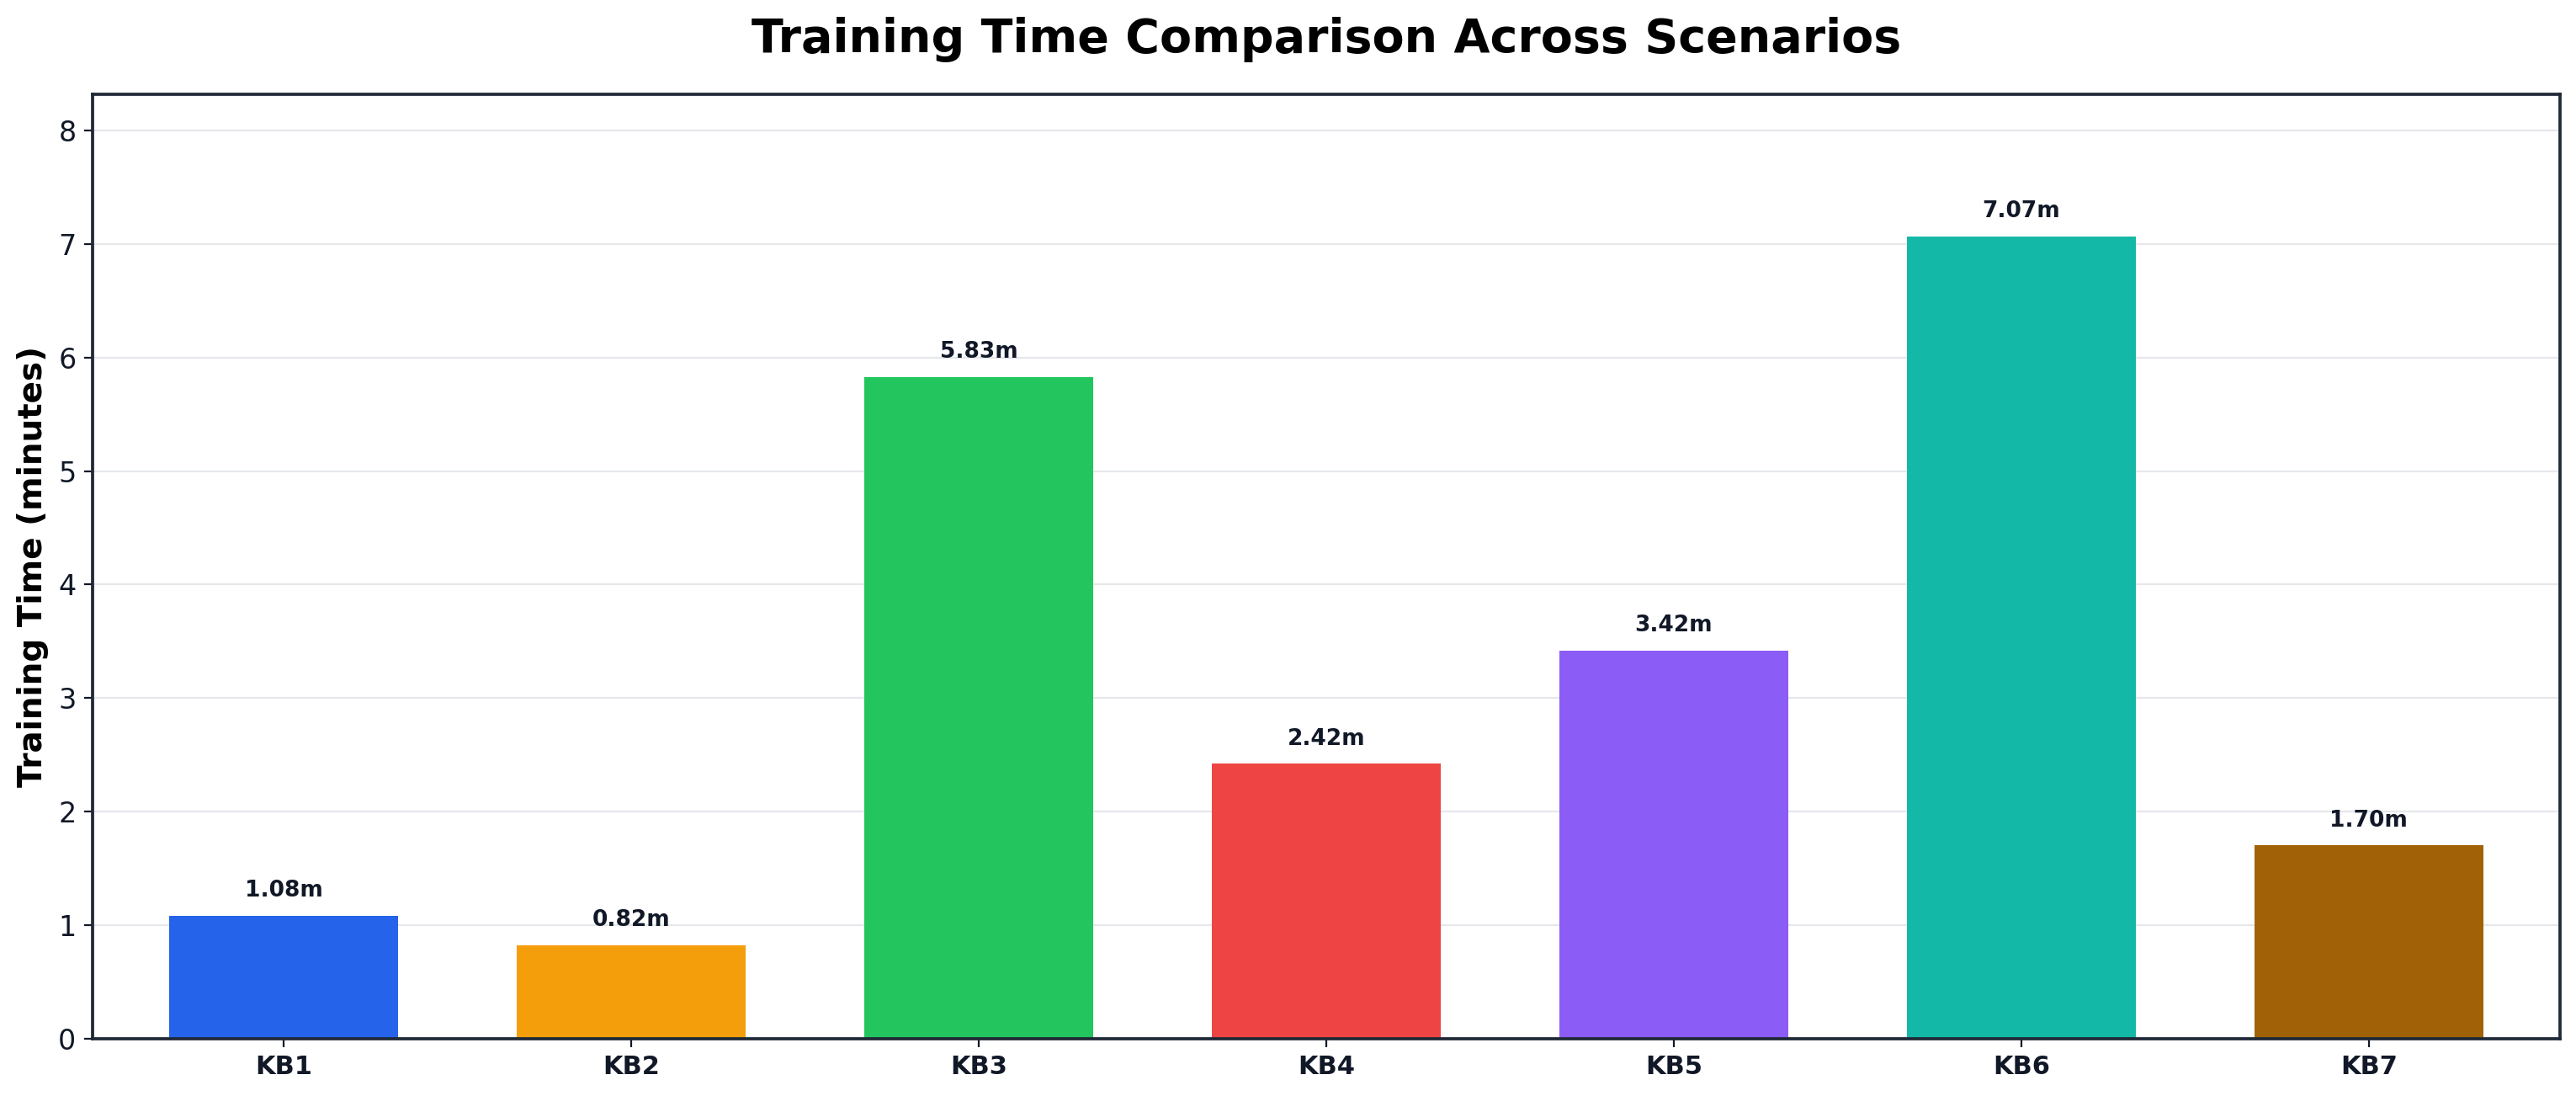
\includegraphics[width=\fairfigurewidth]{acc-loss/metric_training_time_english.png}
    \caption{Training time of the scenarios}
\end{figure}

Training time differs considerably across architectures. T-LSTM and TCN require the longest time, at 7.07 and 5.83 minutes, respectively. PatchTST, LSTM, and GraphSAGE require 3.42, 2.42, and 1.70 minutes, respectively; XGBoost and LightGBM require 0.82 and 1.08 minutes. These results reflect the trade-off between the training cost of sequential models and the speed of boosted tree models in the experimental environment used.

\subsection{Test results}

\subsubsection{Accuracy}
\begin{figure}[H]
    \centering
    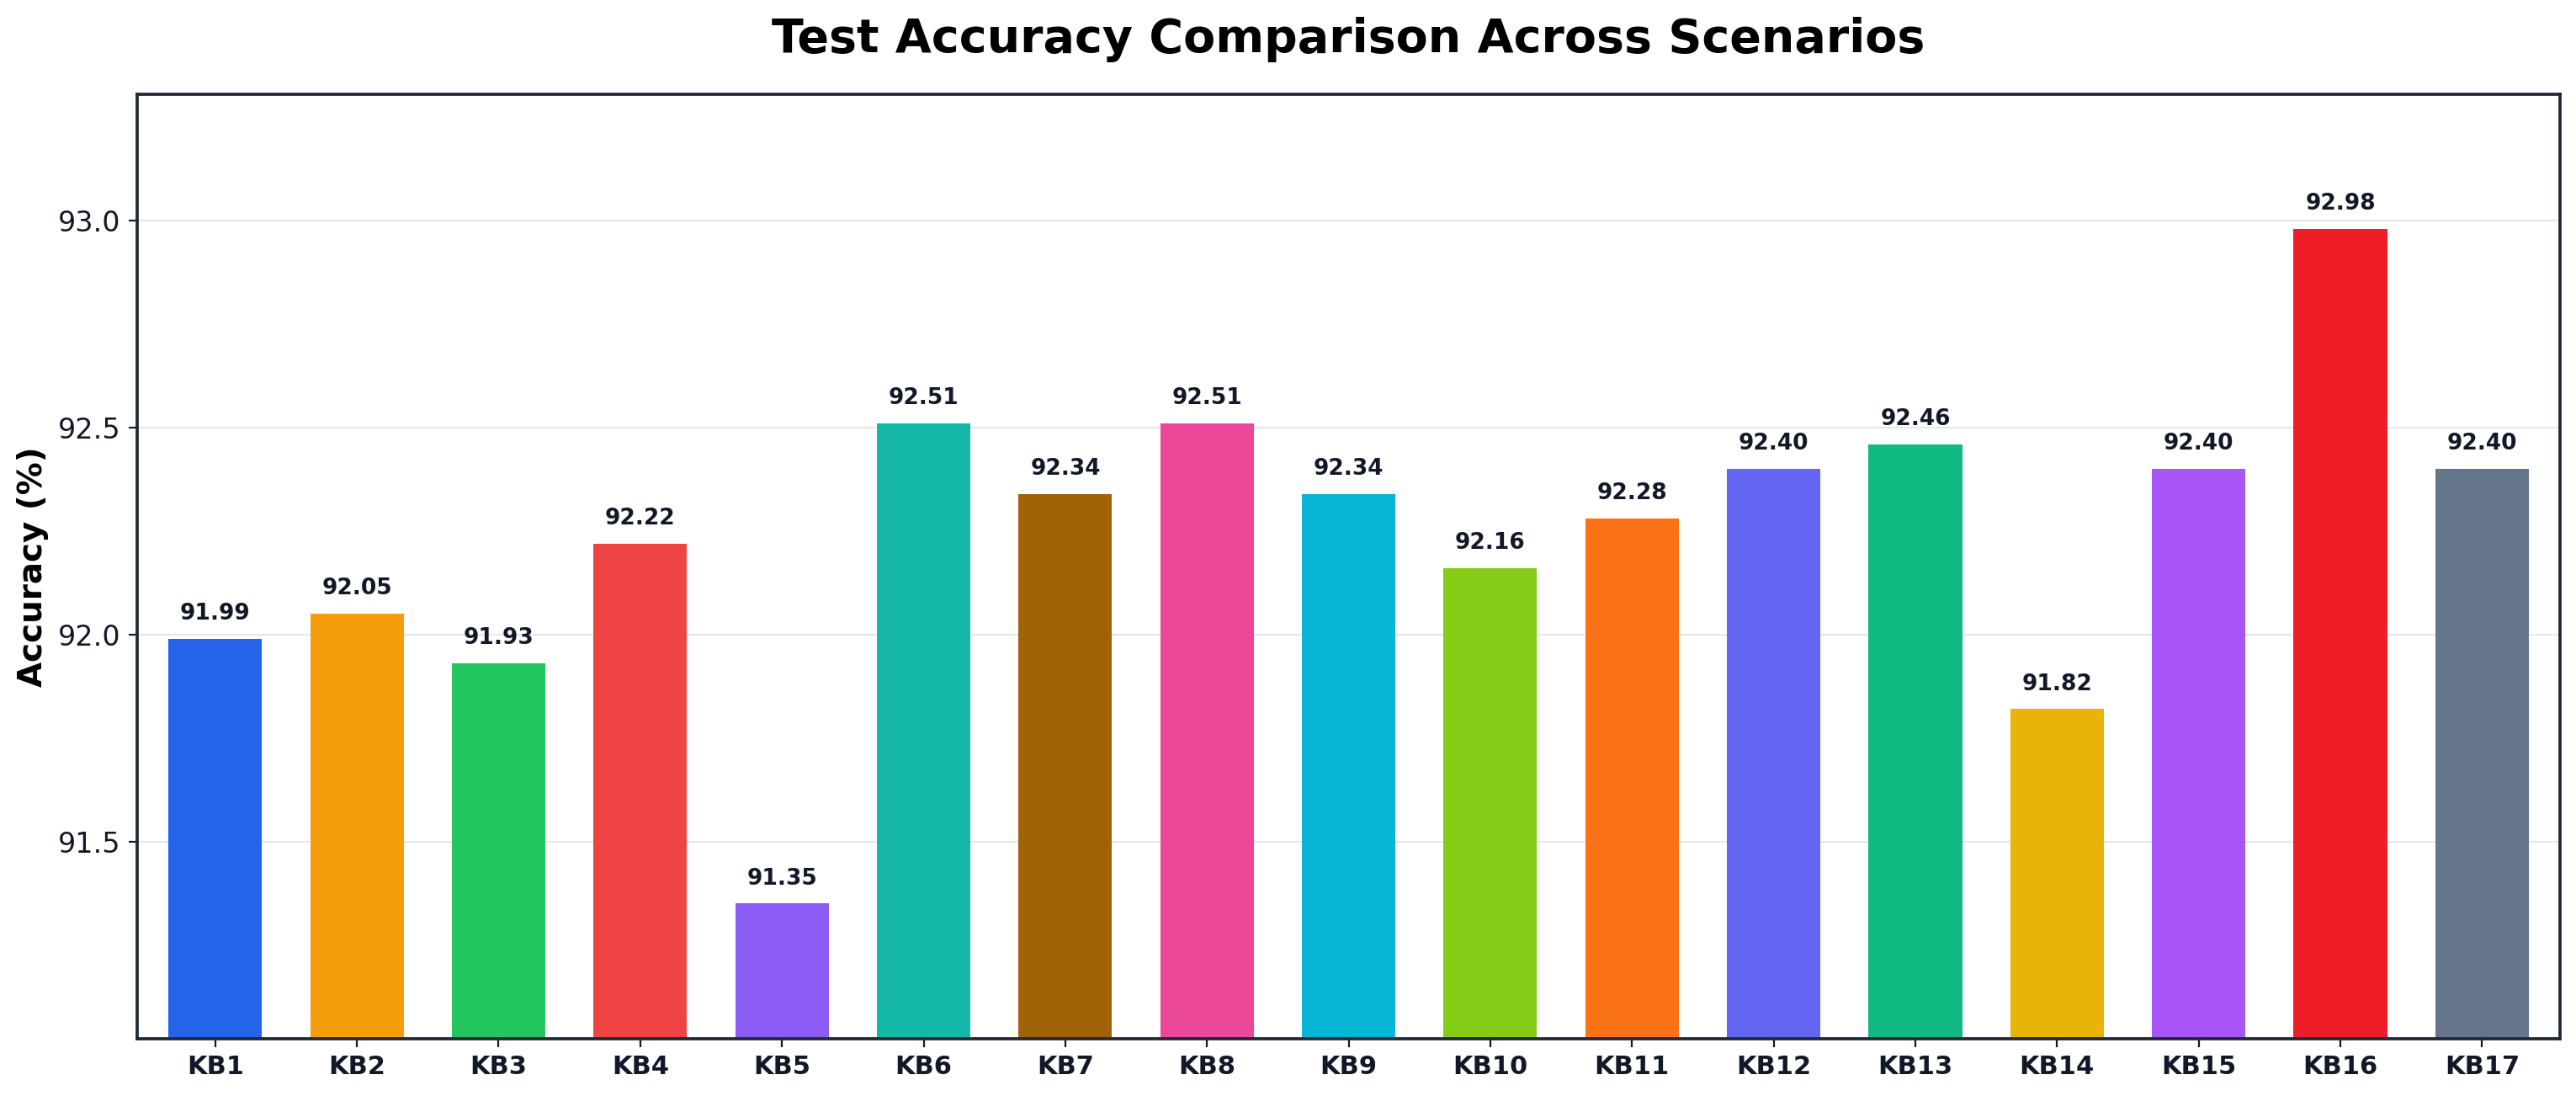
\includegraphics[width=\fairfigurewidth]{acc-loss/metric_accuracy_test_scenarios_english.png}
    \caption{Accuracy chart on the test set}
    \label{tab:acc-test}
\end{figure}
Test Accuracy ranges from 91.35\% to 92.98\%. Among individual models, T-LSTM achieves the highest value (92.51\%), followed by GraphSAGE (92.34\%) and LSTM (92.22\%). FI-TTX also reaches 92.51\%, while FR-TTLPXL achieves 92.46\%. DMF obtains the highest Accuracy among all 14 scenarios, at 92.98\%. This result indicates the potential benefit of dynamic selection; however, further testing is required to determine the statistical significance of the difference.

\subsubsection{Precision of the scenarios}

\begin{figure}[H]
\centering
\setupfairsubfigures
\begin{subfigure}{\fairfigurewidth}
    \centering
    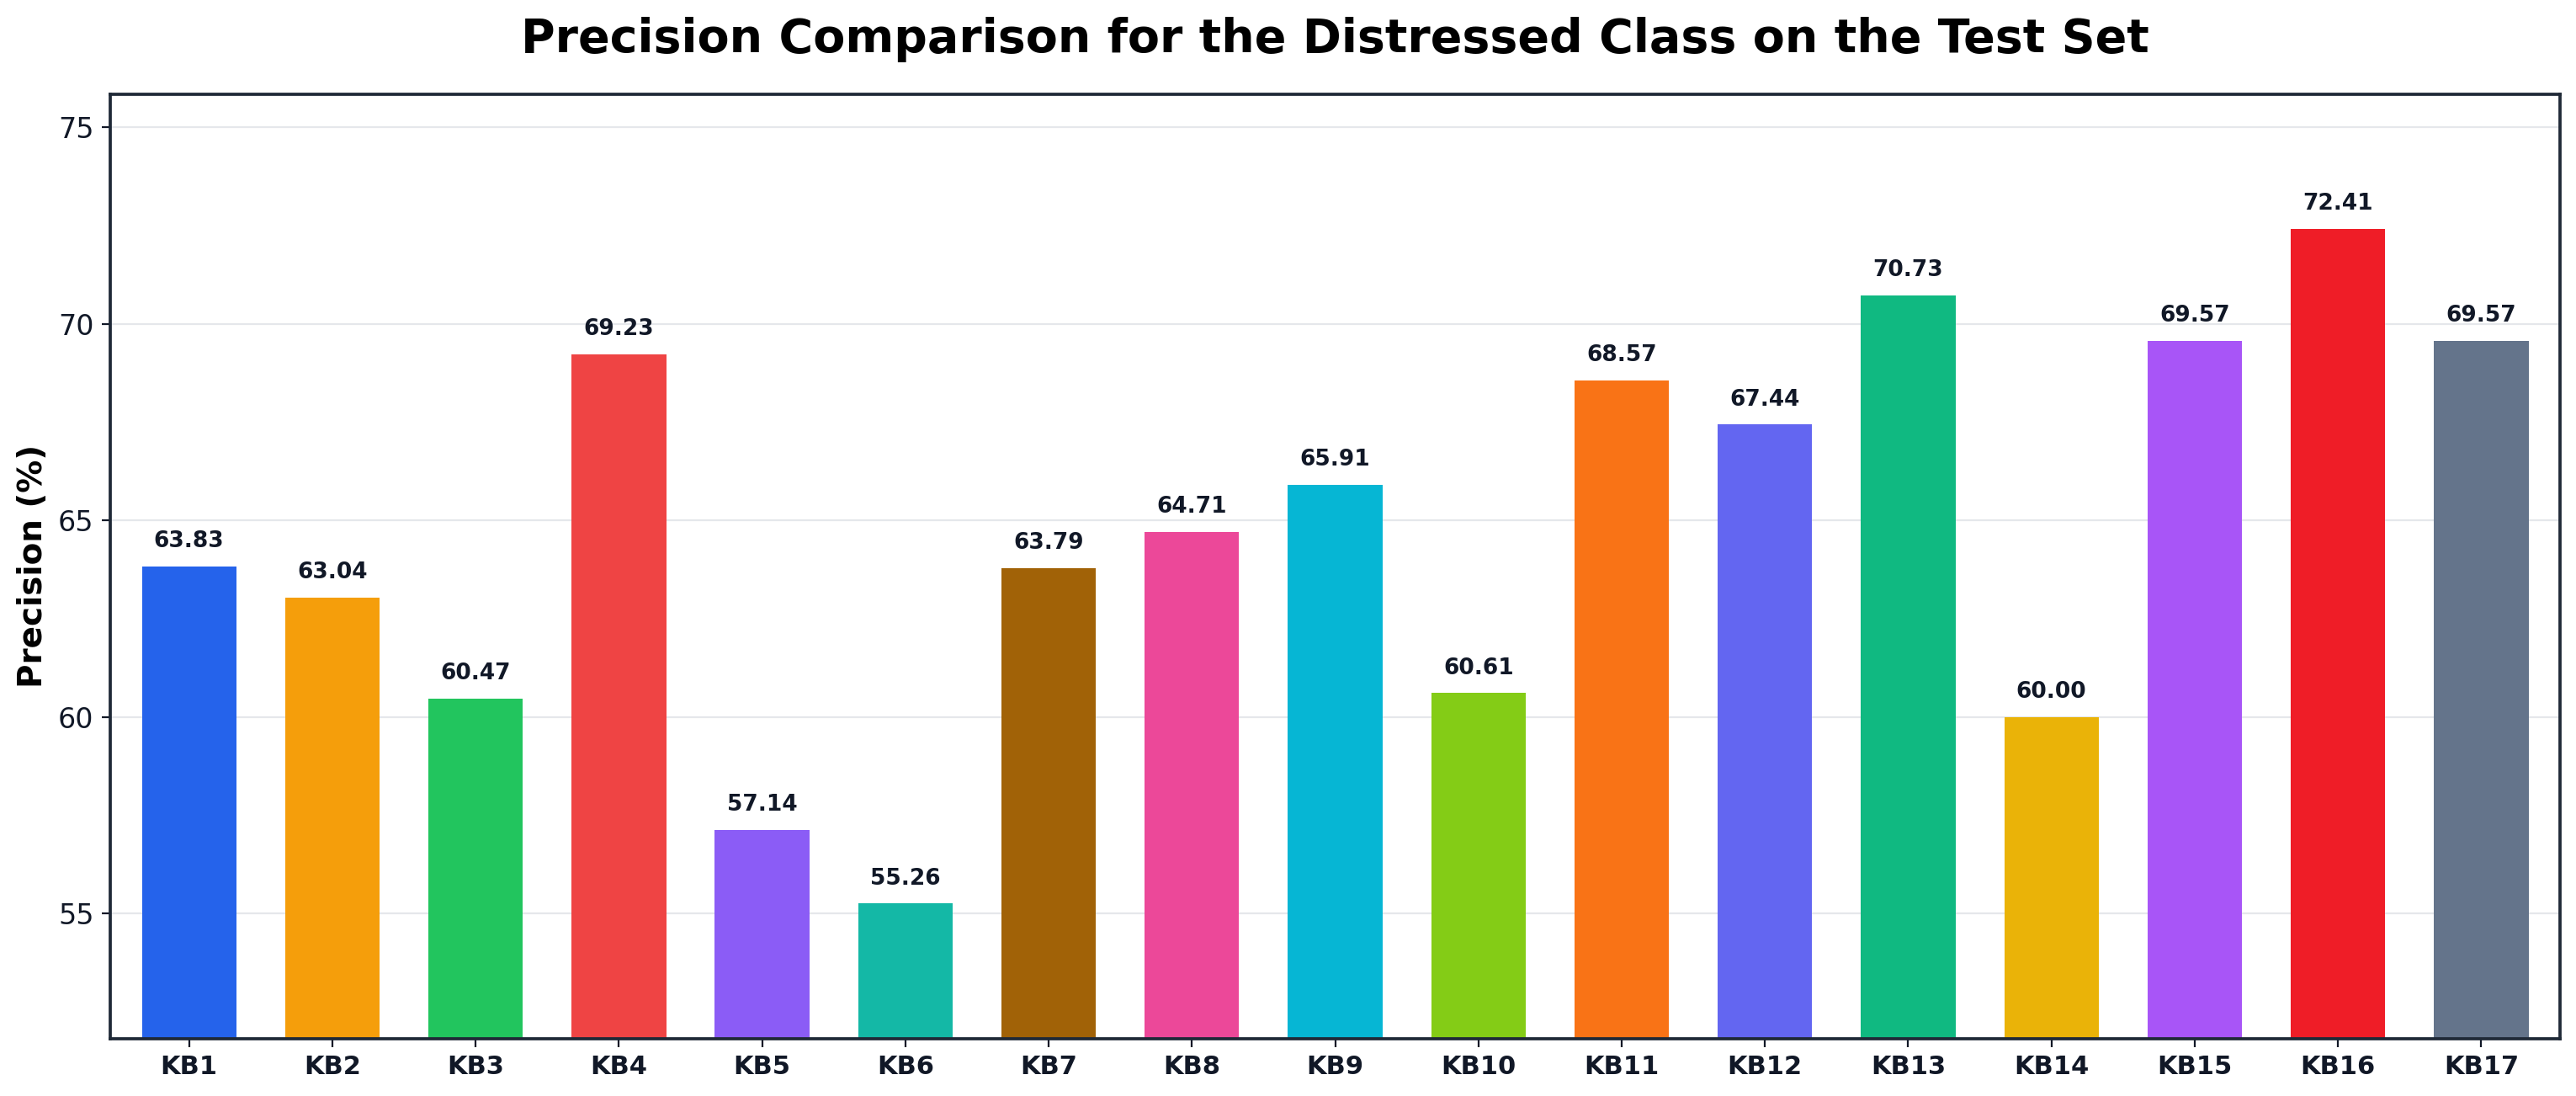
\includegraphics[width=\textwidth]{acc-loss/metric_precision_distressed_test_english.png}
    \caption{Precision of the Distressed class}
    \label{fig:precision_distressed}
\end{subfigure}
\end{figure}

\begin{figure}[H]
\ContinuedFloat
\centering
\begin{subfigure}{\fairfigurewidth}
    \centering
    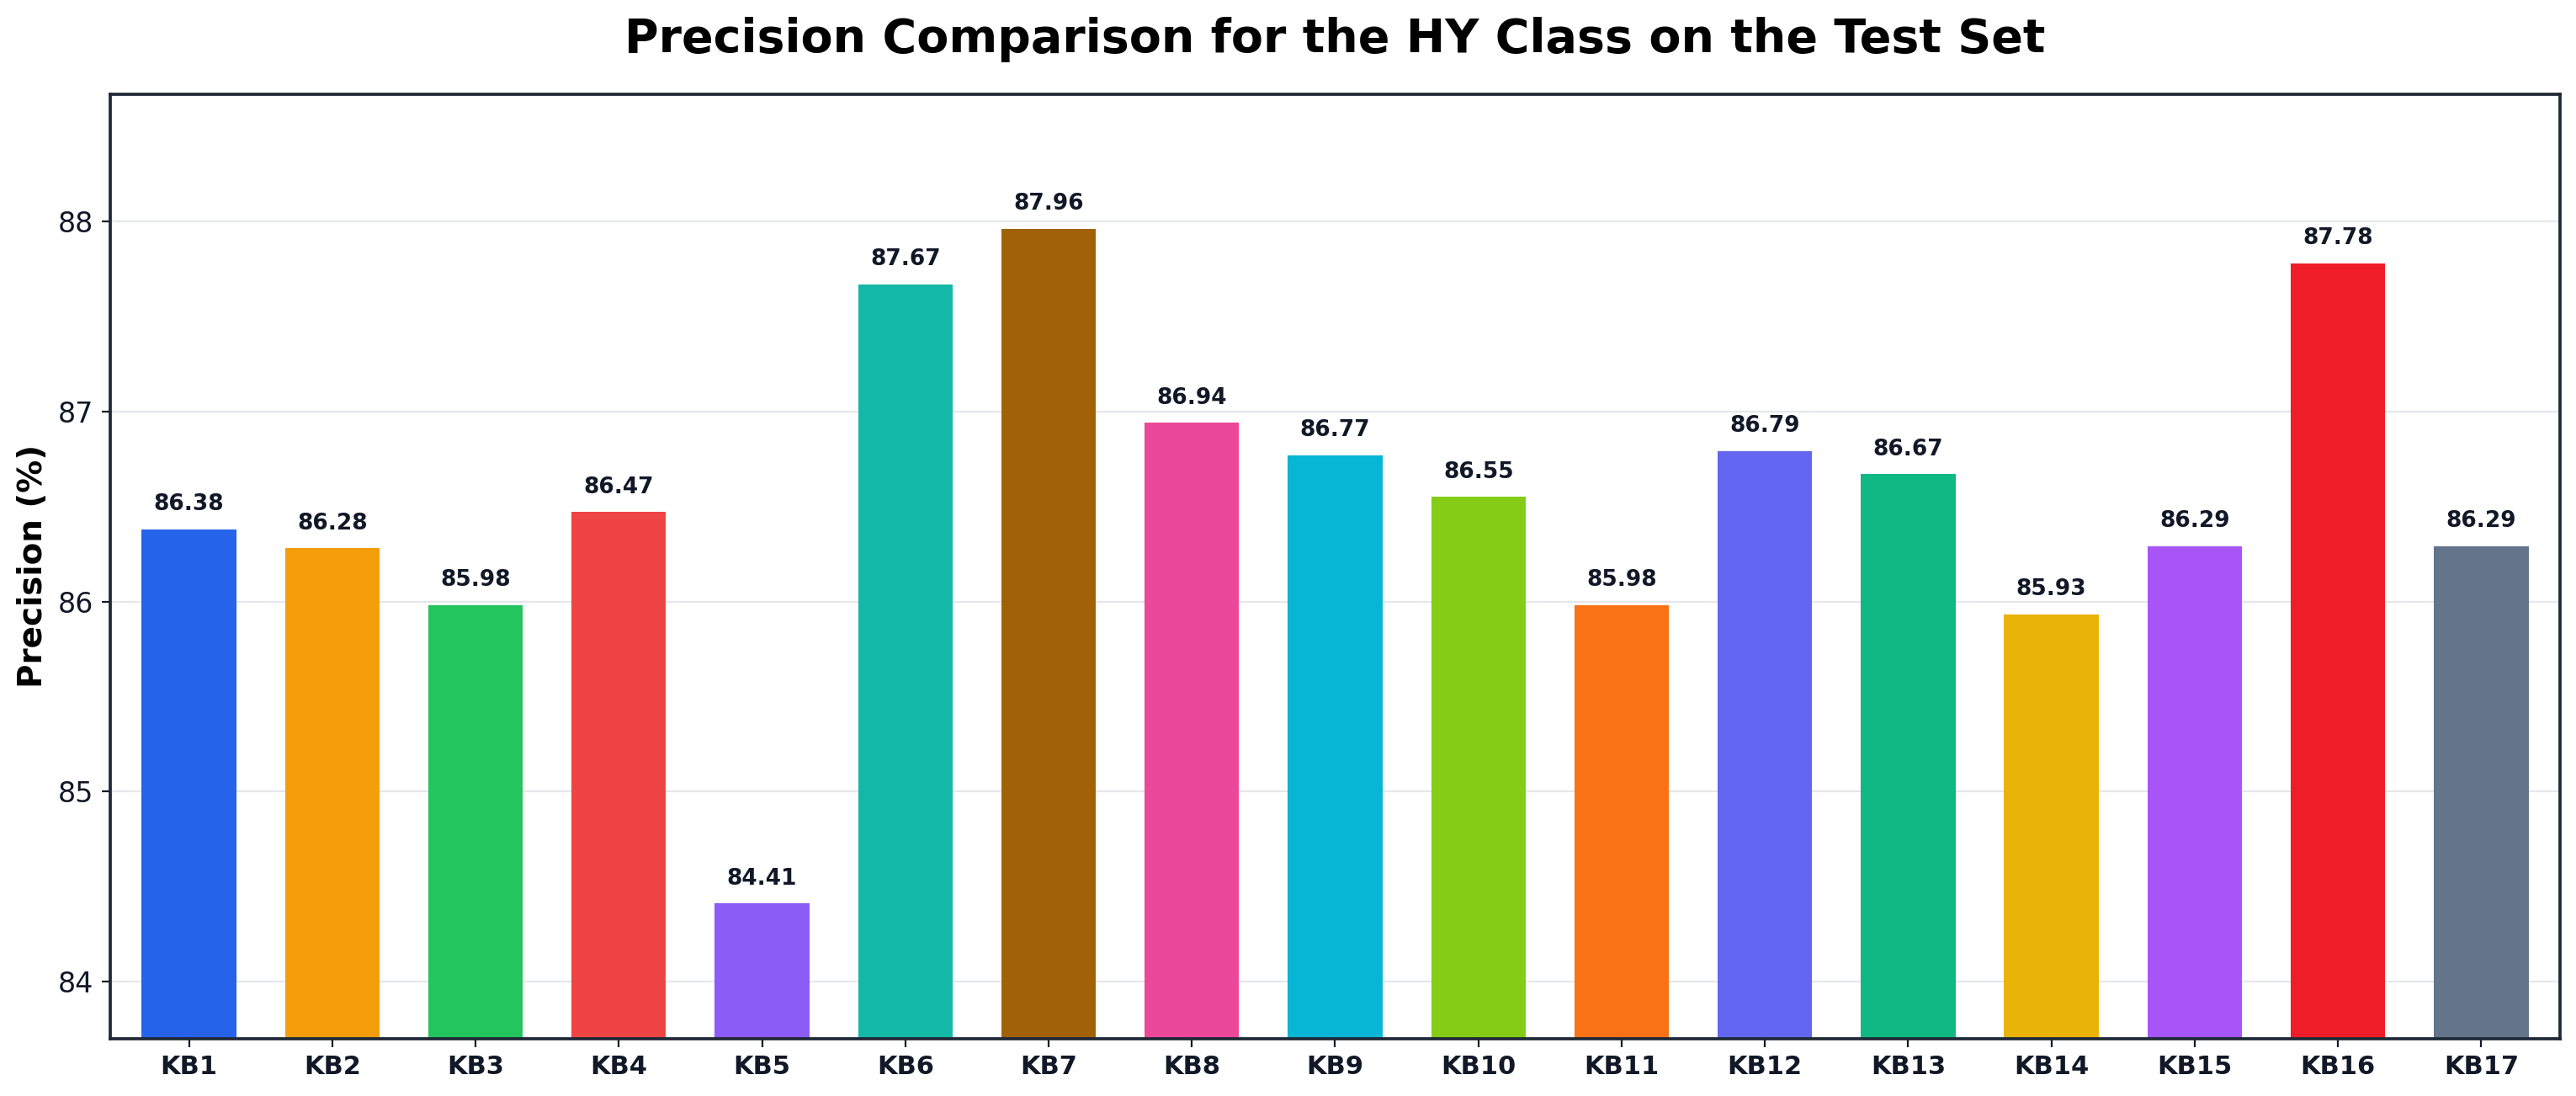
\includegraphics[width=\textwidth]{acc-loss/metric_precision_hy_test_english.png}
    \caption{Precision of the HY class (High Yield)}
    \label{fig:precision_hy}
\end{subfigure}
\end{figure}

\begin{figure}[H]
\ContinuedFloat
\centering
\begin{subfigure}{\fairfigurewidth}
    \centering
    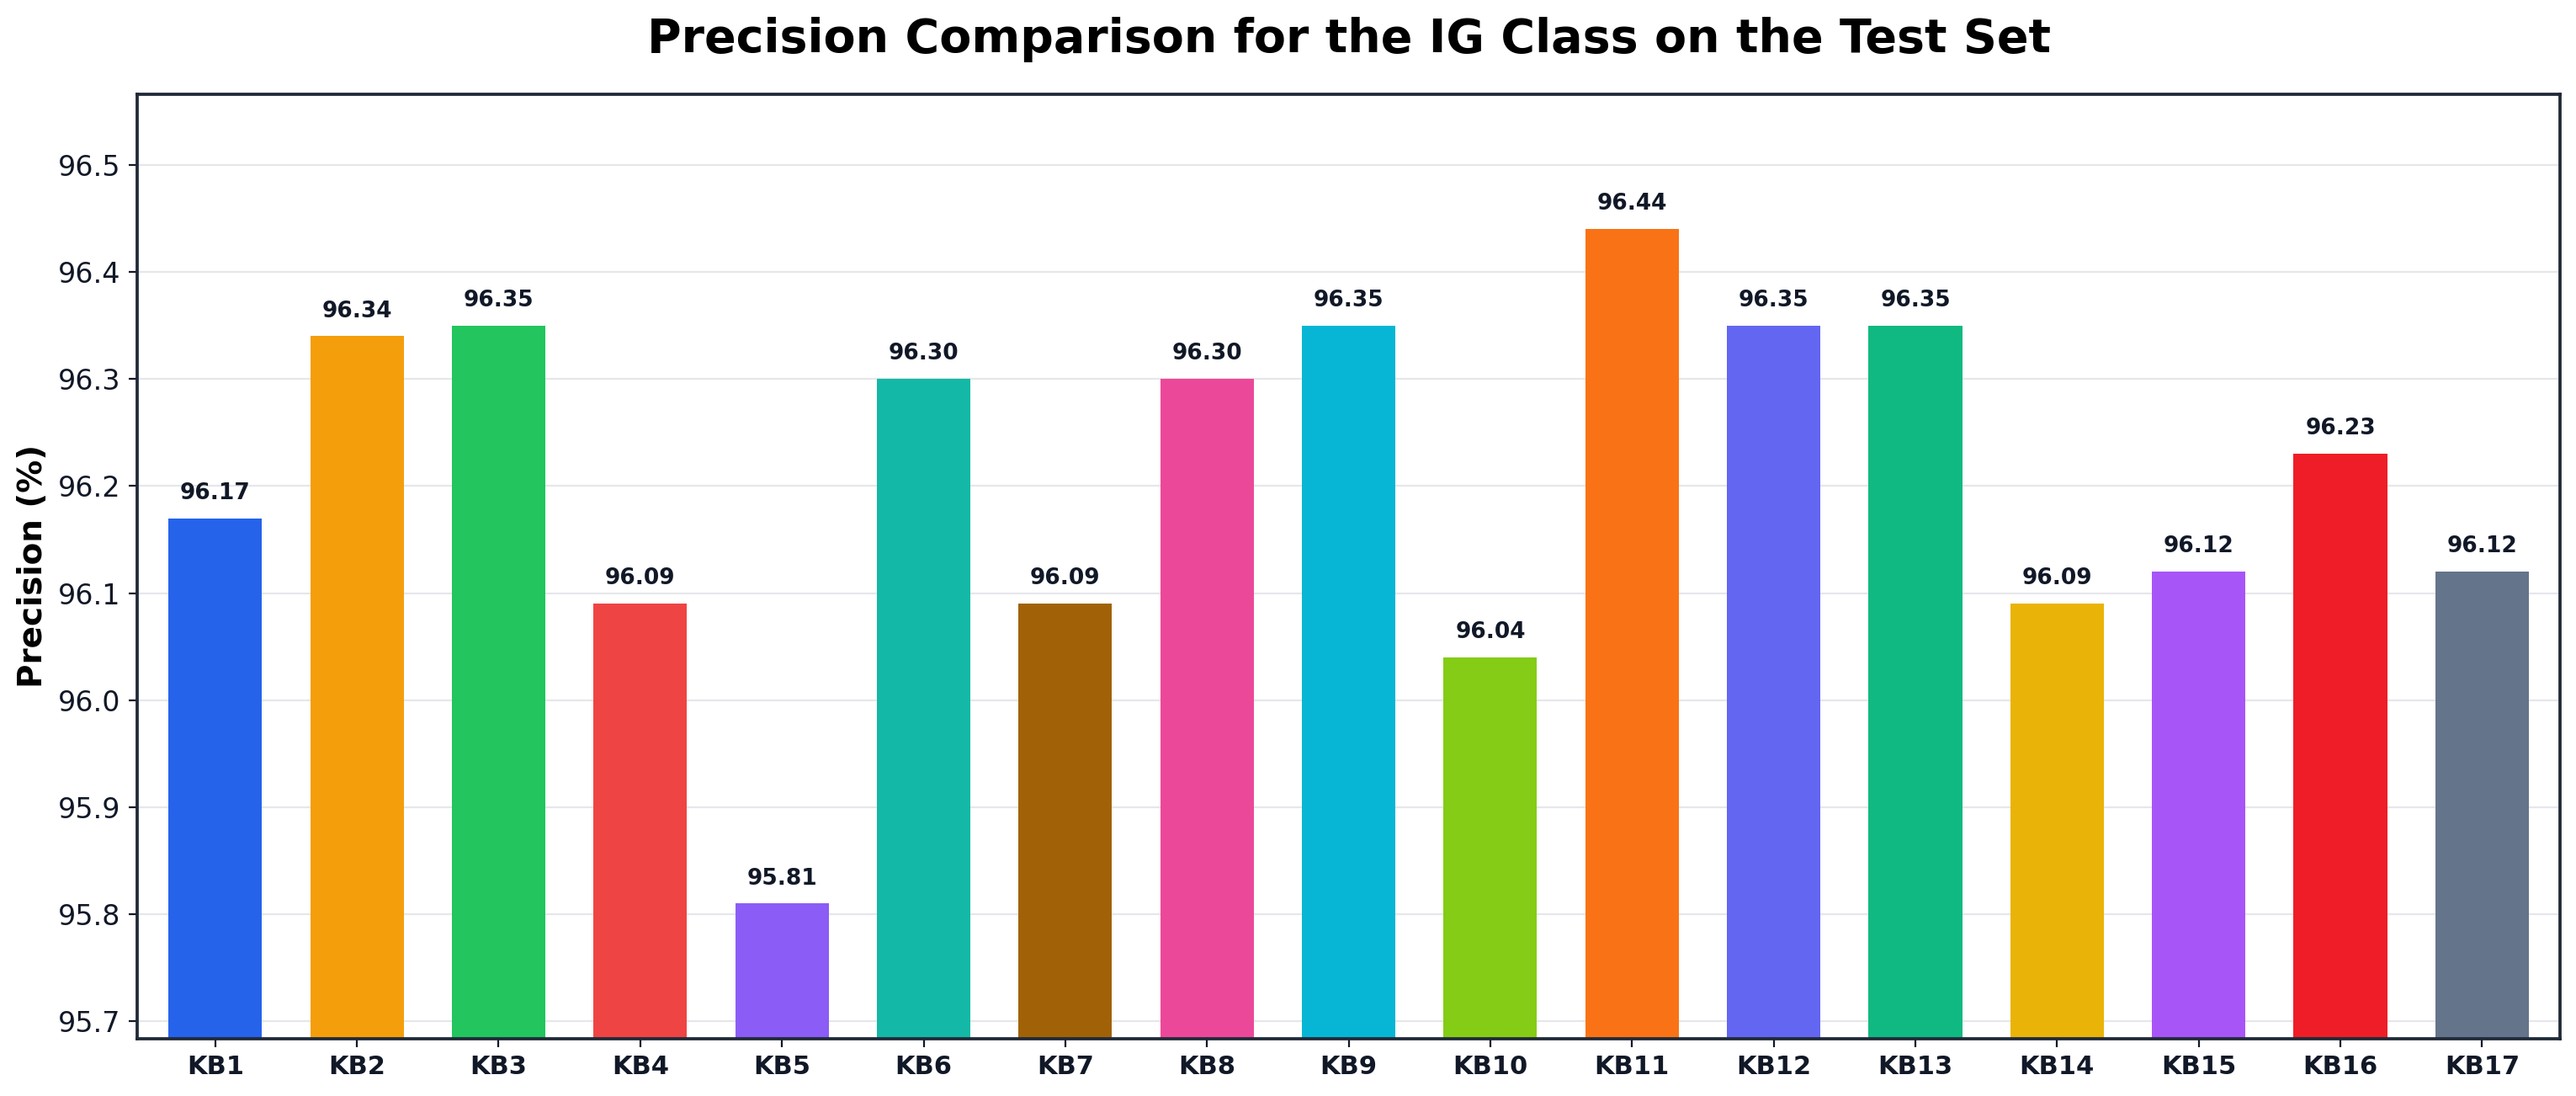
\includegraphics[width=\textwidth]{acc-loss/metric_precision_ig_test_english.png}
    \caption{Precision of the IG class (Investment Grade)}
    \label{fig:precision_ig}
\end{subfigure}
\caption{Precision of the Distressed class (a), HY class (b), and IG class (c) on the test set}
\label{fig:precision_classes}
\end{figure}
Precision varies across rating classes. For the Distressed class, DMF achieves the highest value (72.41\%), followed by FR-TTLPXL (70.73\%) and LSTM (69.23\%). For the HY class, Precision ranges from 84.41\% to 87.96\%; GraphSAGE reaches 87.96\%, DMF reaches 87.78\%, and T-LSTM reaches 87.67\%. For the IG class, values range from 95.81\% to 96.44\%, with FR-TTX achieving the highest value. The differences among classes indicate that overall Precision should be interpreted together with class-level metrics, especially for the Distressed group.

\subsubsection{Recall of the scenarios}
\begin{figure}[H]
\centering
\setupfairsubfigures
\begin{subfigure}{\fairfigurewidth}
    \centering
    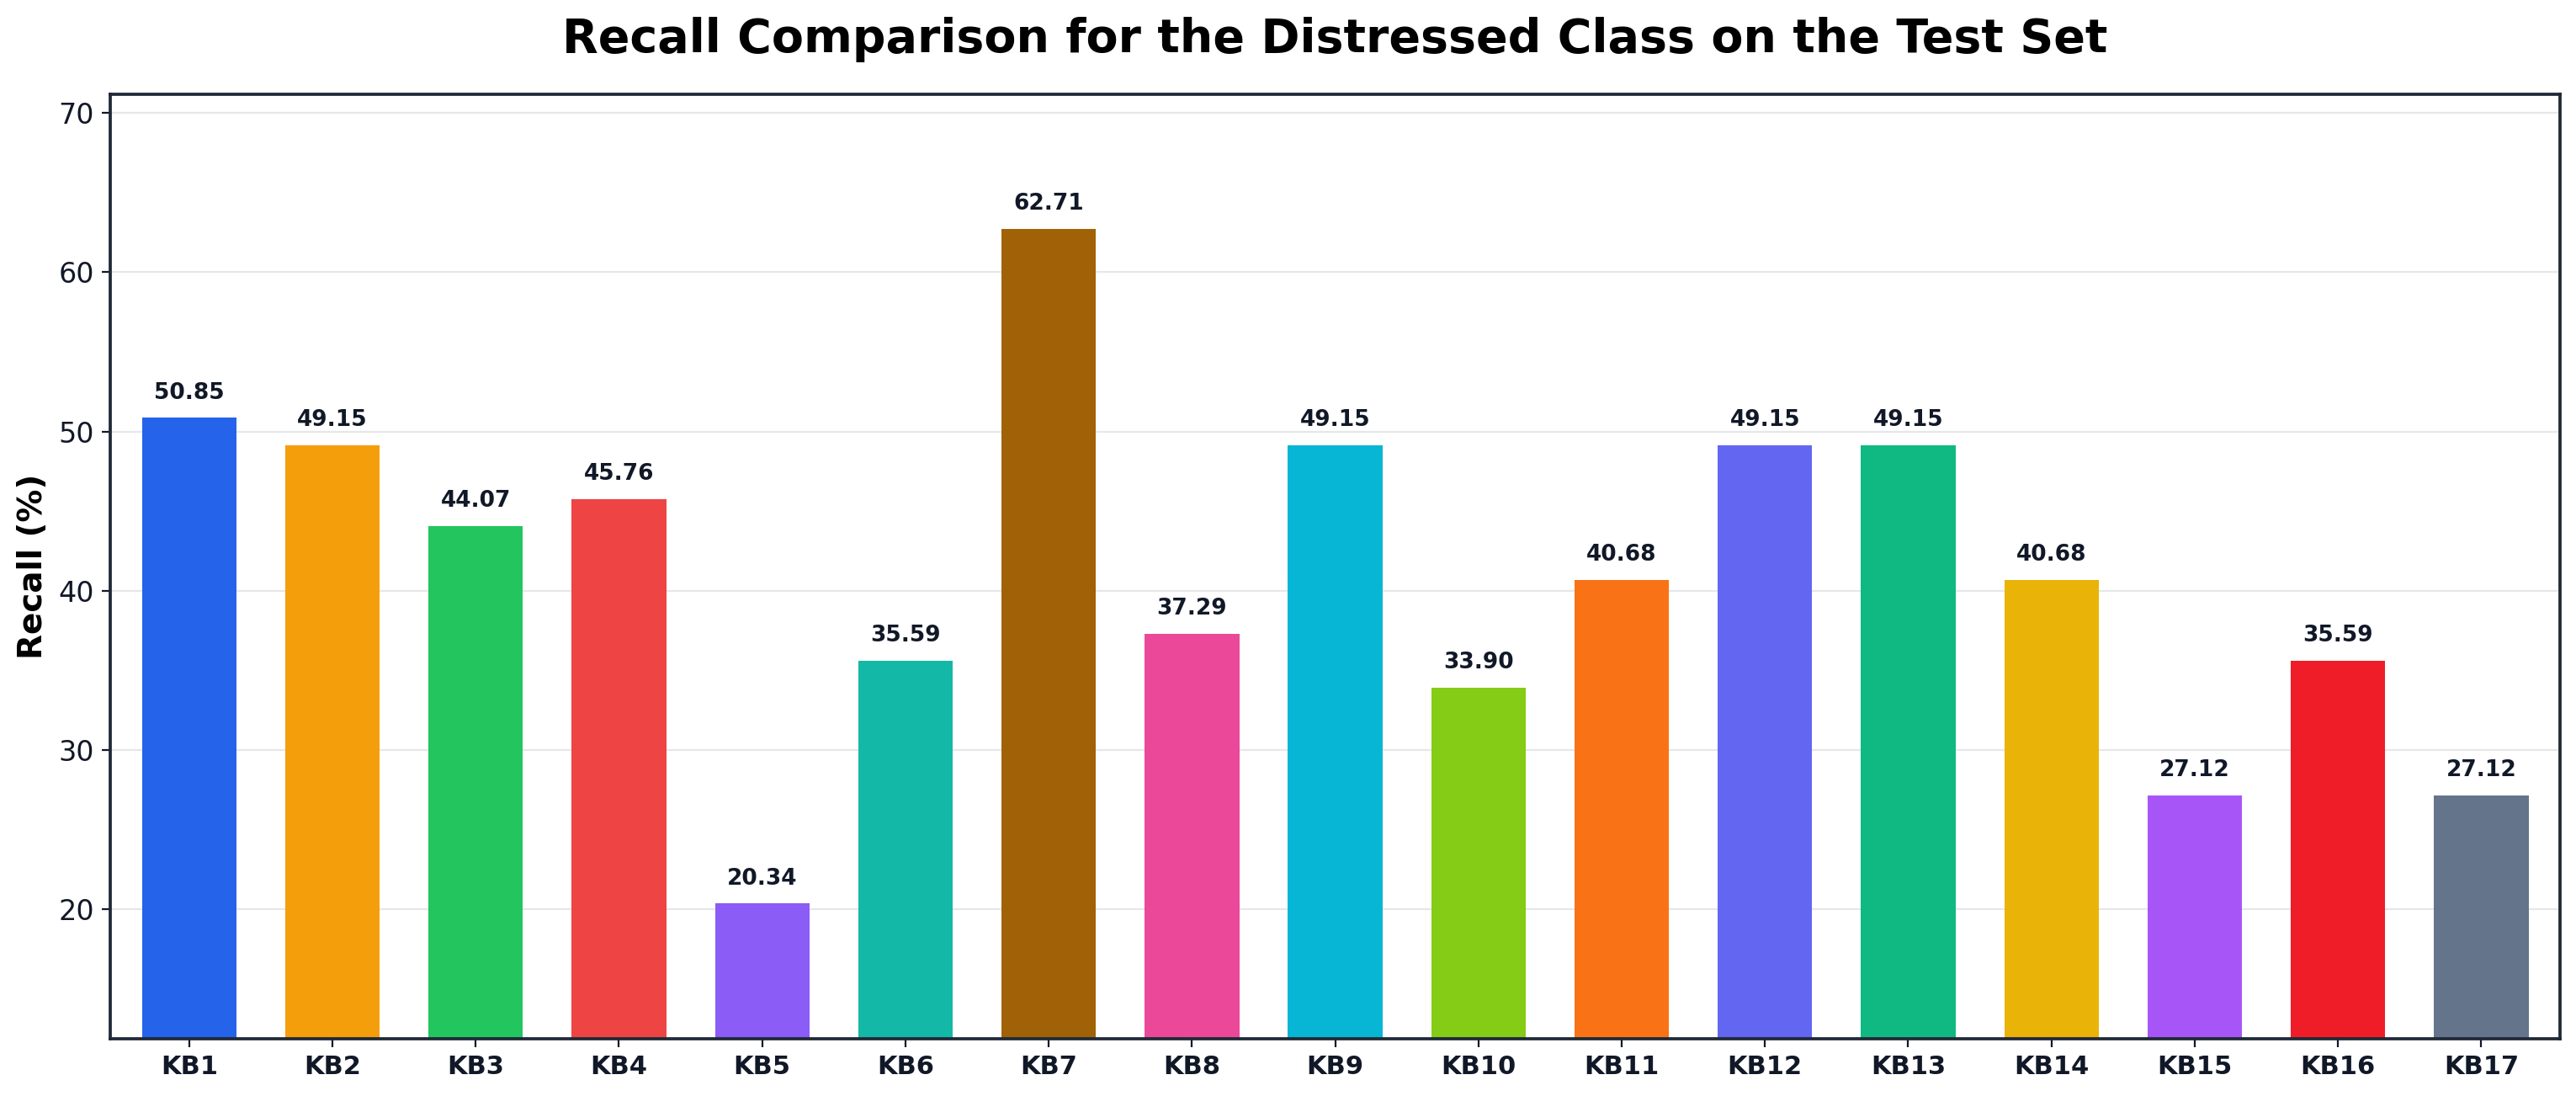
\includegraphics[width=\textwidth]{acc-loss/metric_recall_distressed_test_english.png}
    \caption{Recall of the Distressed class}
    \label{fig:Recall_distressed}
\end{subfigure}
\end{figure}

\begin{figure}[H]
\ContinuedFloat
\centering
\begin{subfigure}{\fairfigurewidth}
    \centering
    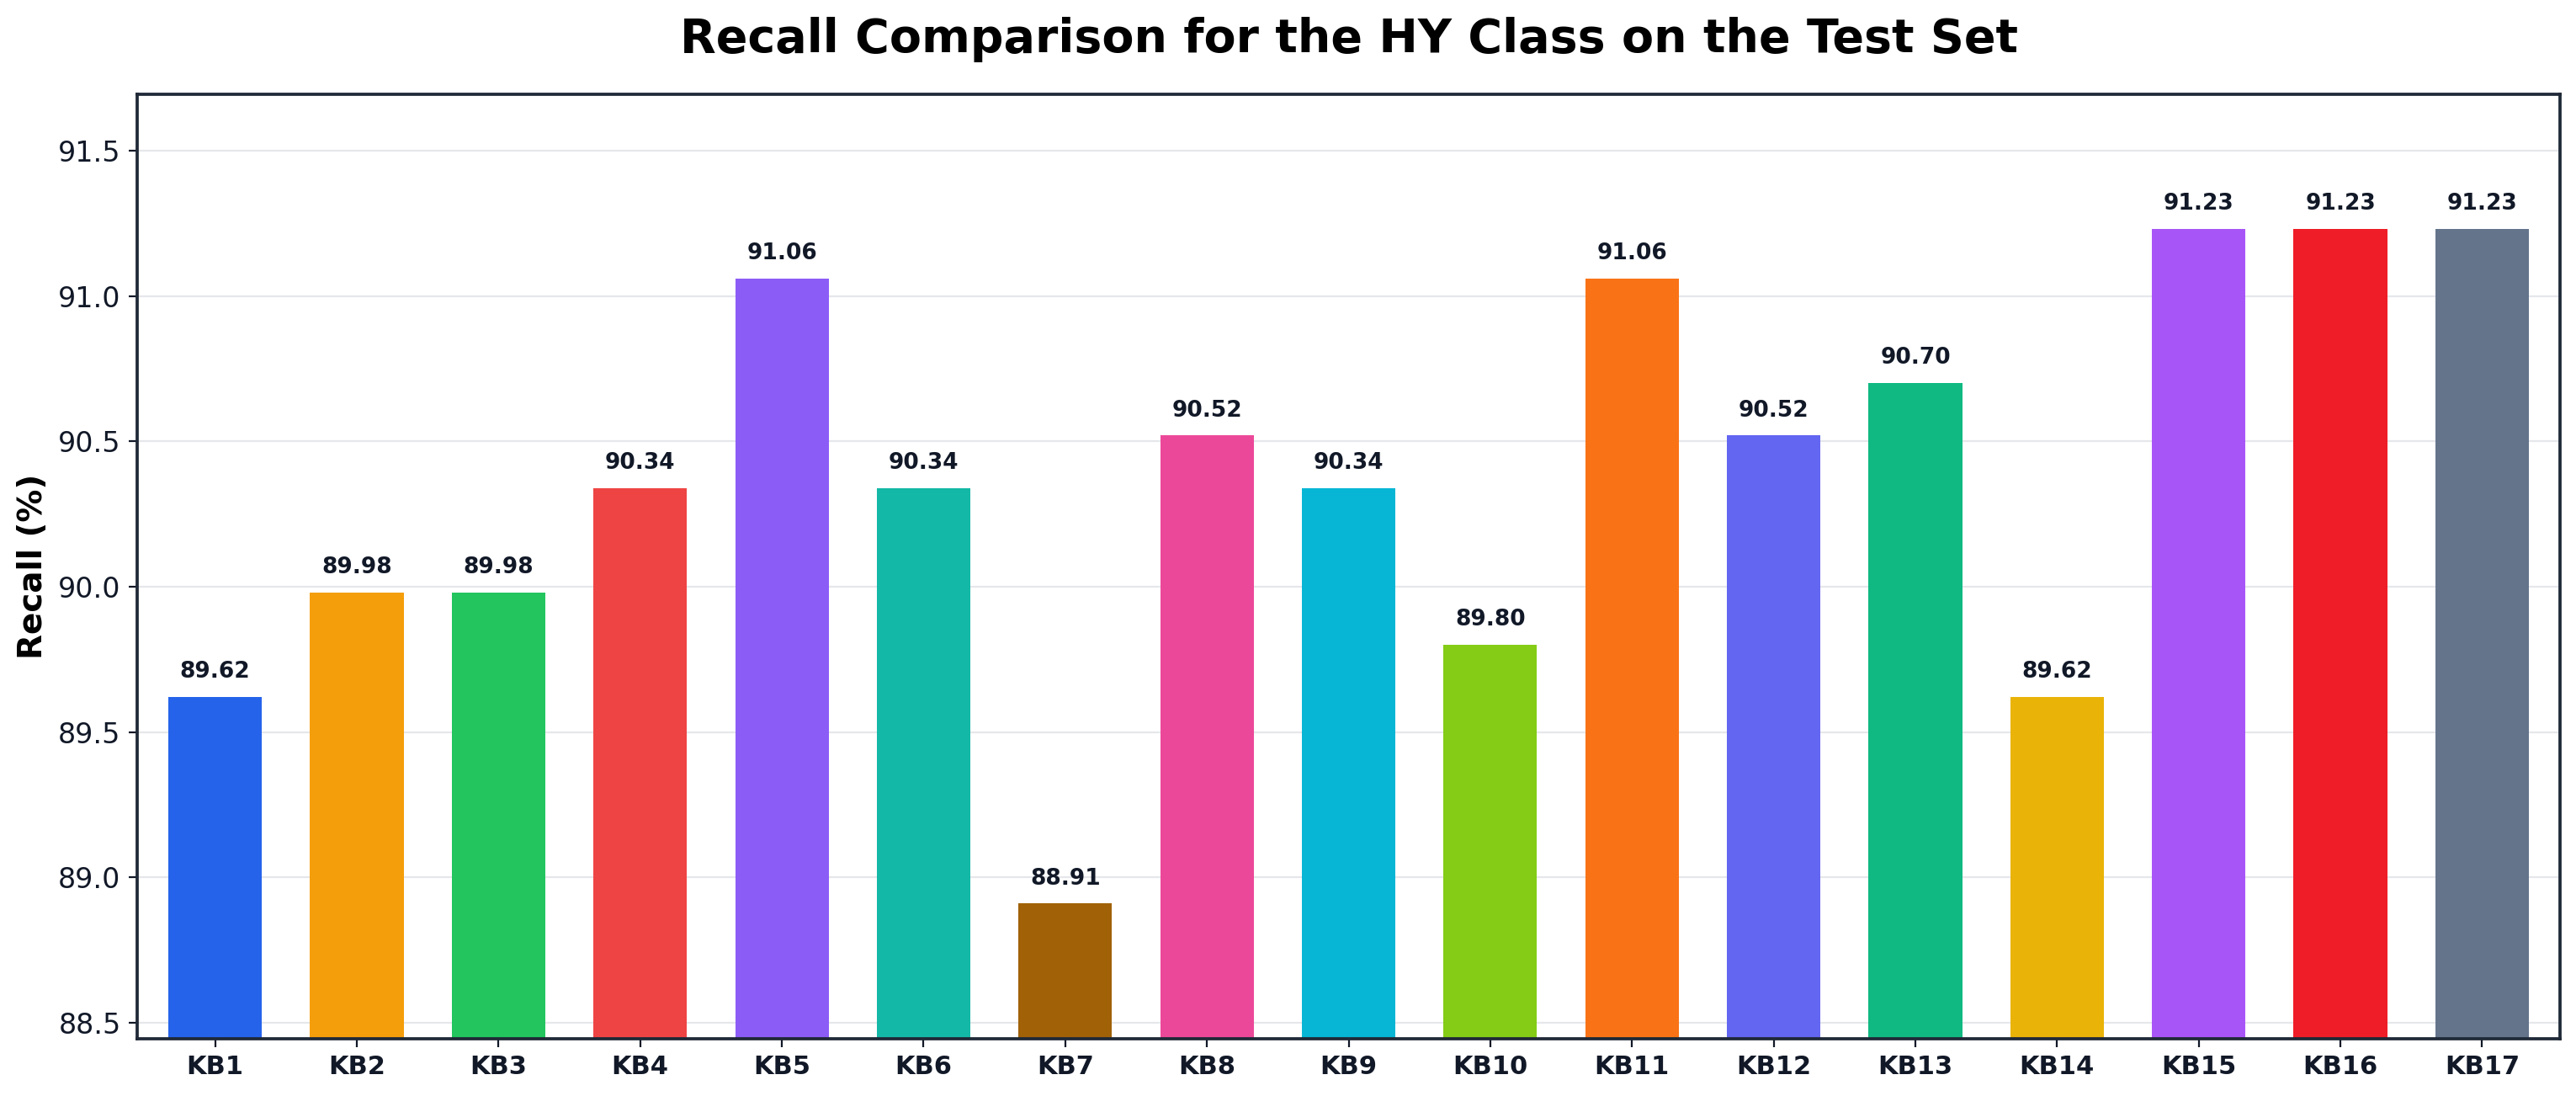
\includegraphics[width=\textwidth]{acc-loss/metric_recall_hy_test_english.png}
    \caption{Recall of the HY class (High Yield)}
    \label{fig:Recall_hy}
\end{subfigure}
\end{figure}

\begin{figure}[H]
\ContinuedFloat
\centering
\begin{subfigure}{\fairfigurewidth}
    \centering
    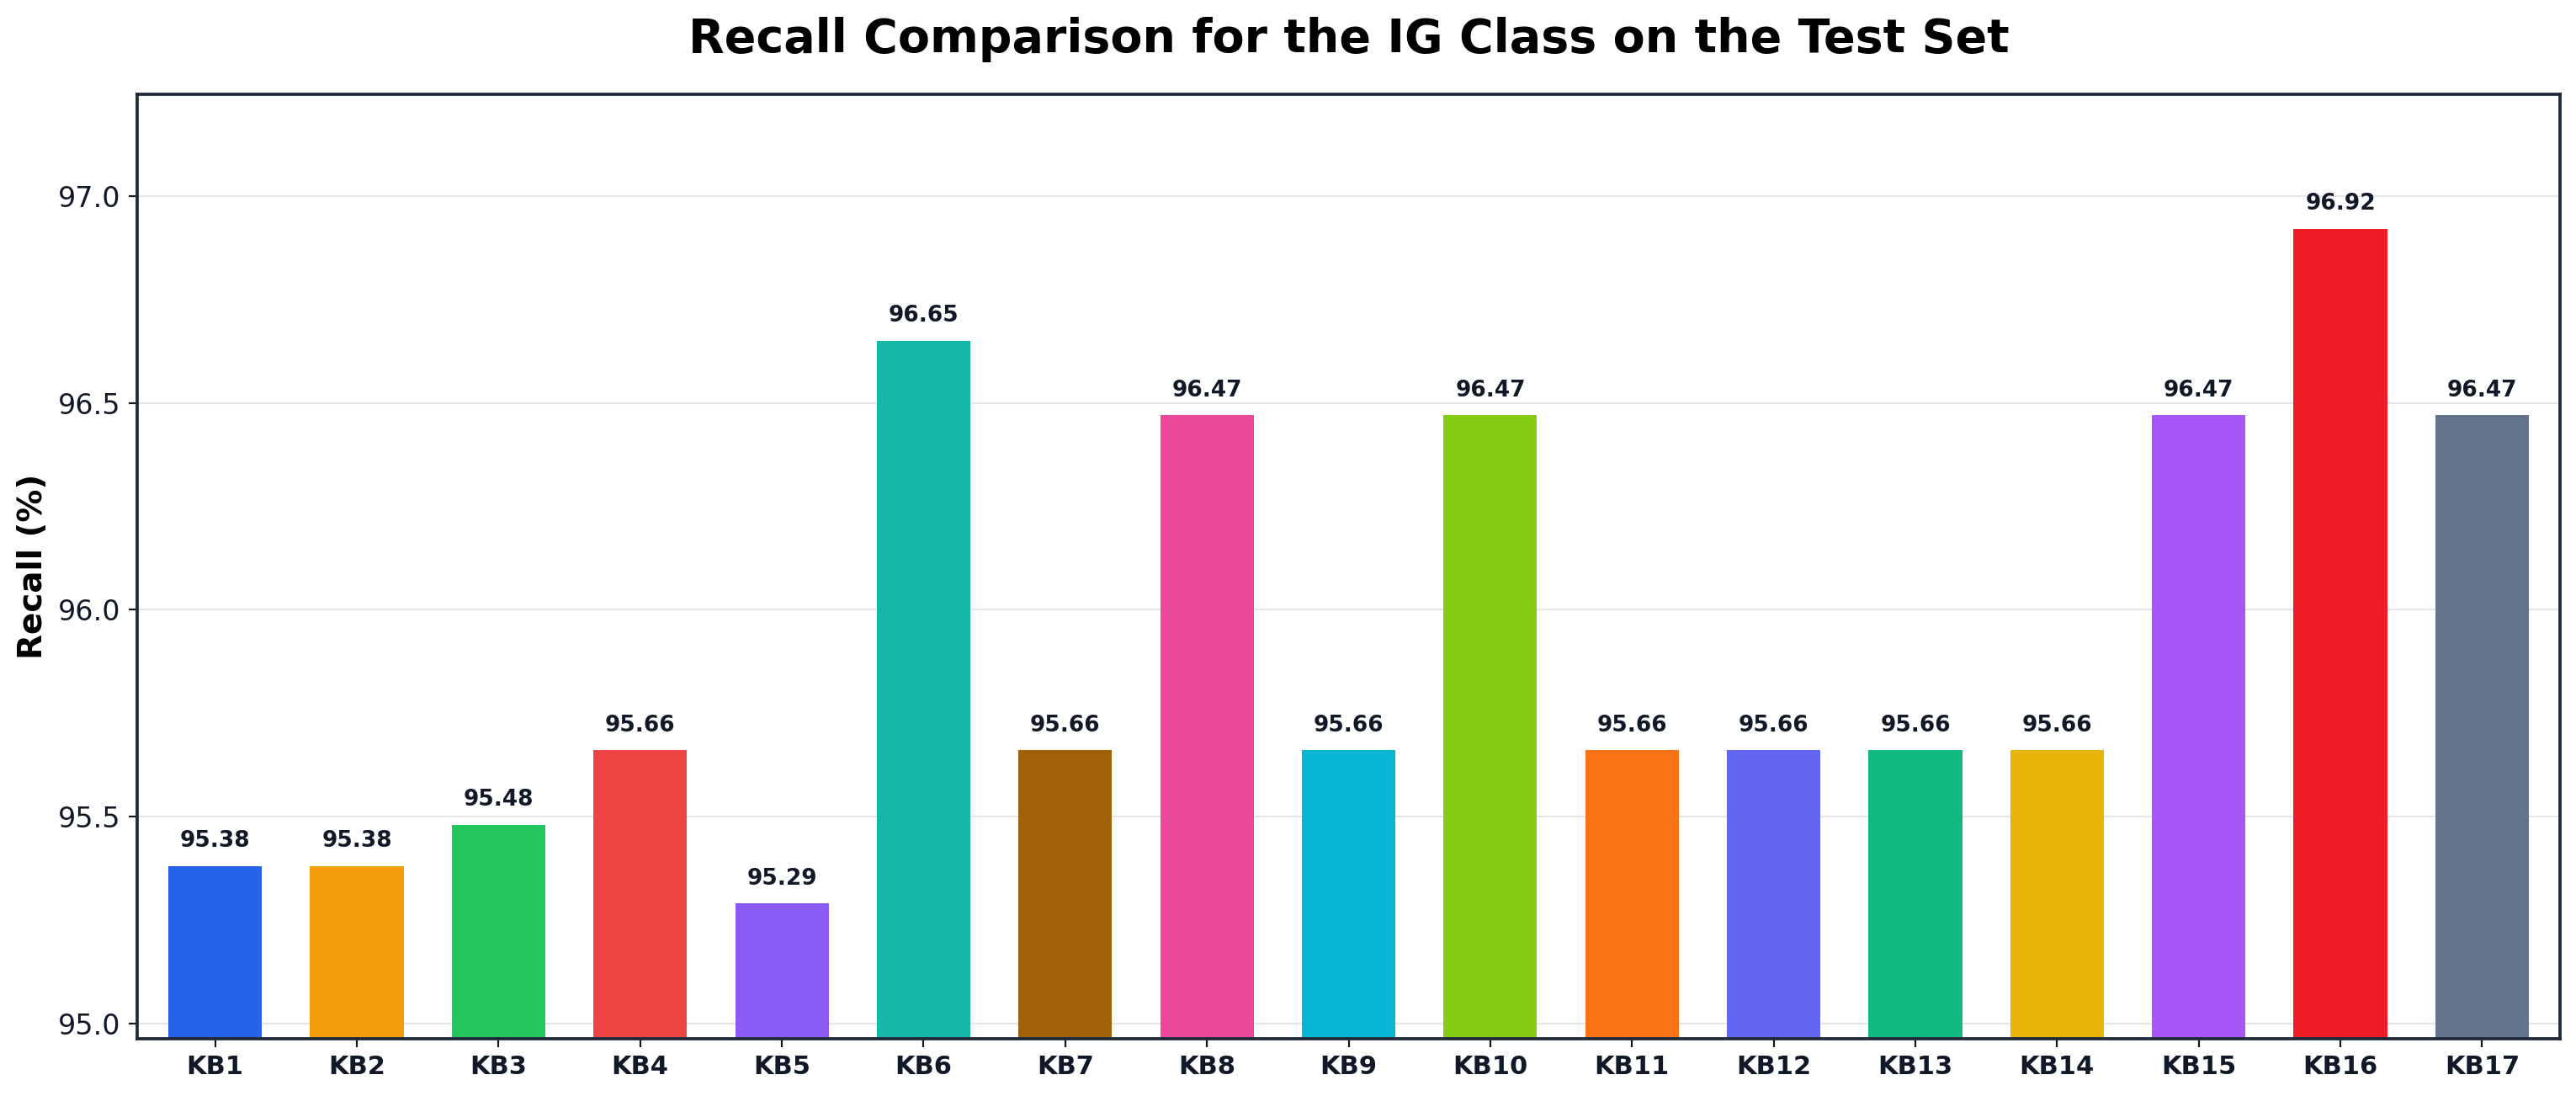
\includegraphics[width=\textwidth]{acc-loss/metric_recall_ig_test_english.png}
    \caption{Recall of the IG class (Investment Grade)}
    \label{fig:Recall_ig}
\end{subfigure}
\caption{Recall of the Distressed class (a), HY class (b), and IG class (c) on the test set}
\label{fig:Recall_classes}
\end{figure}
Recall shows the largest difference for the Distressed class. GraphSAGE achieves a Recall of 62.71\%, higher than LightGBM (50.85\%), XGBoost (49.15\%), and DMF (35.59\%); PatchTST records the lowest value at 20.34\%. For the HY class, Recall mainly ranges from 89\% to 91\%, with DMF reaching 91.23\%. For the IG class, the models achieve values from 95.29\% to 96.92\%, with DMF obtaining the highest value. These results show that the Distressed class remains the main limitation of the system and is not fully reflected by overall Accuracy.

\subsubsection{F1-score of the scenarios}
\begin{figure}[H]
\centering
\setupfairsubfigures
\begin{subfigure}{\fairfigurewidth}
    \centering
    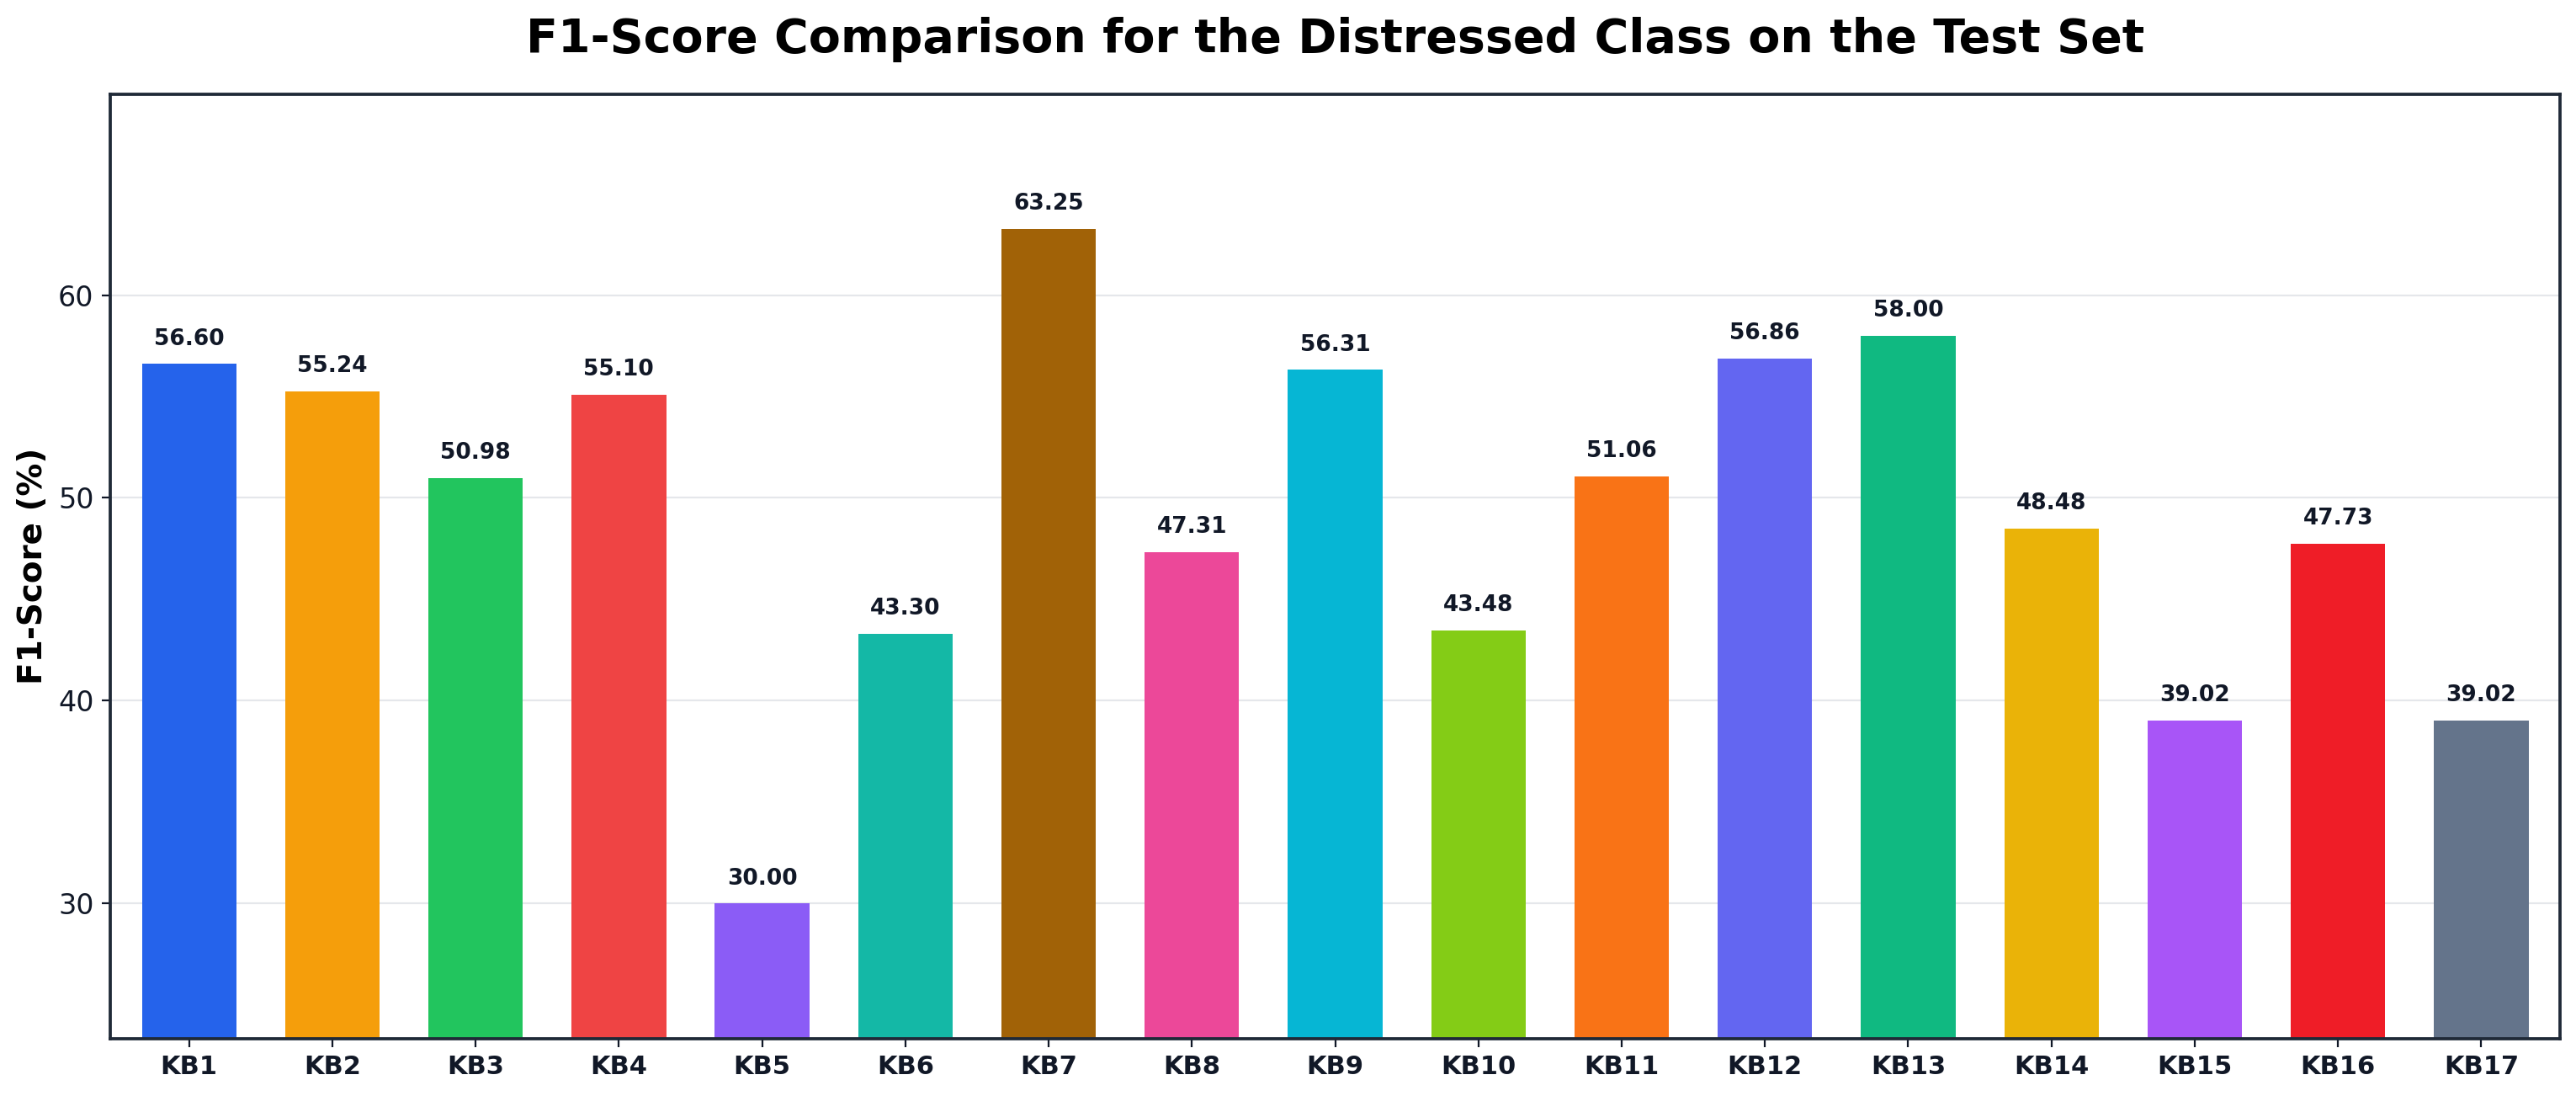
\includegraphics[width=\textwidth]{acc-loss/metric_f1_distressed_test_english.png}
    \caption{F1-score of the Distressed class}
    \label{fig:F1-Score_distressed}
\end{subfigure}
\end{figure}

\begin{figure}[H]
\ContinuedFloat
\centering
\begin{subfigure}{\fairfigurewidth}
    \centering
    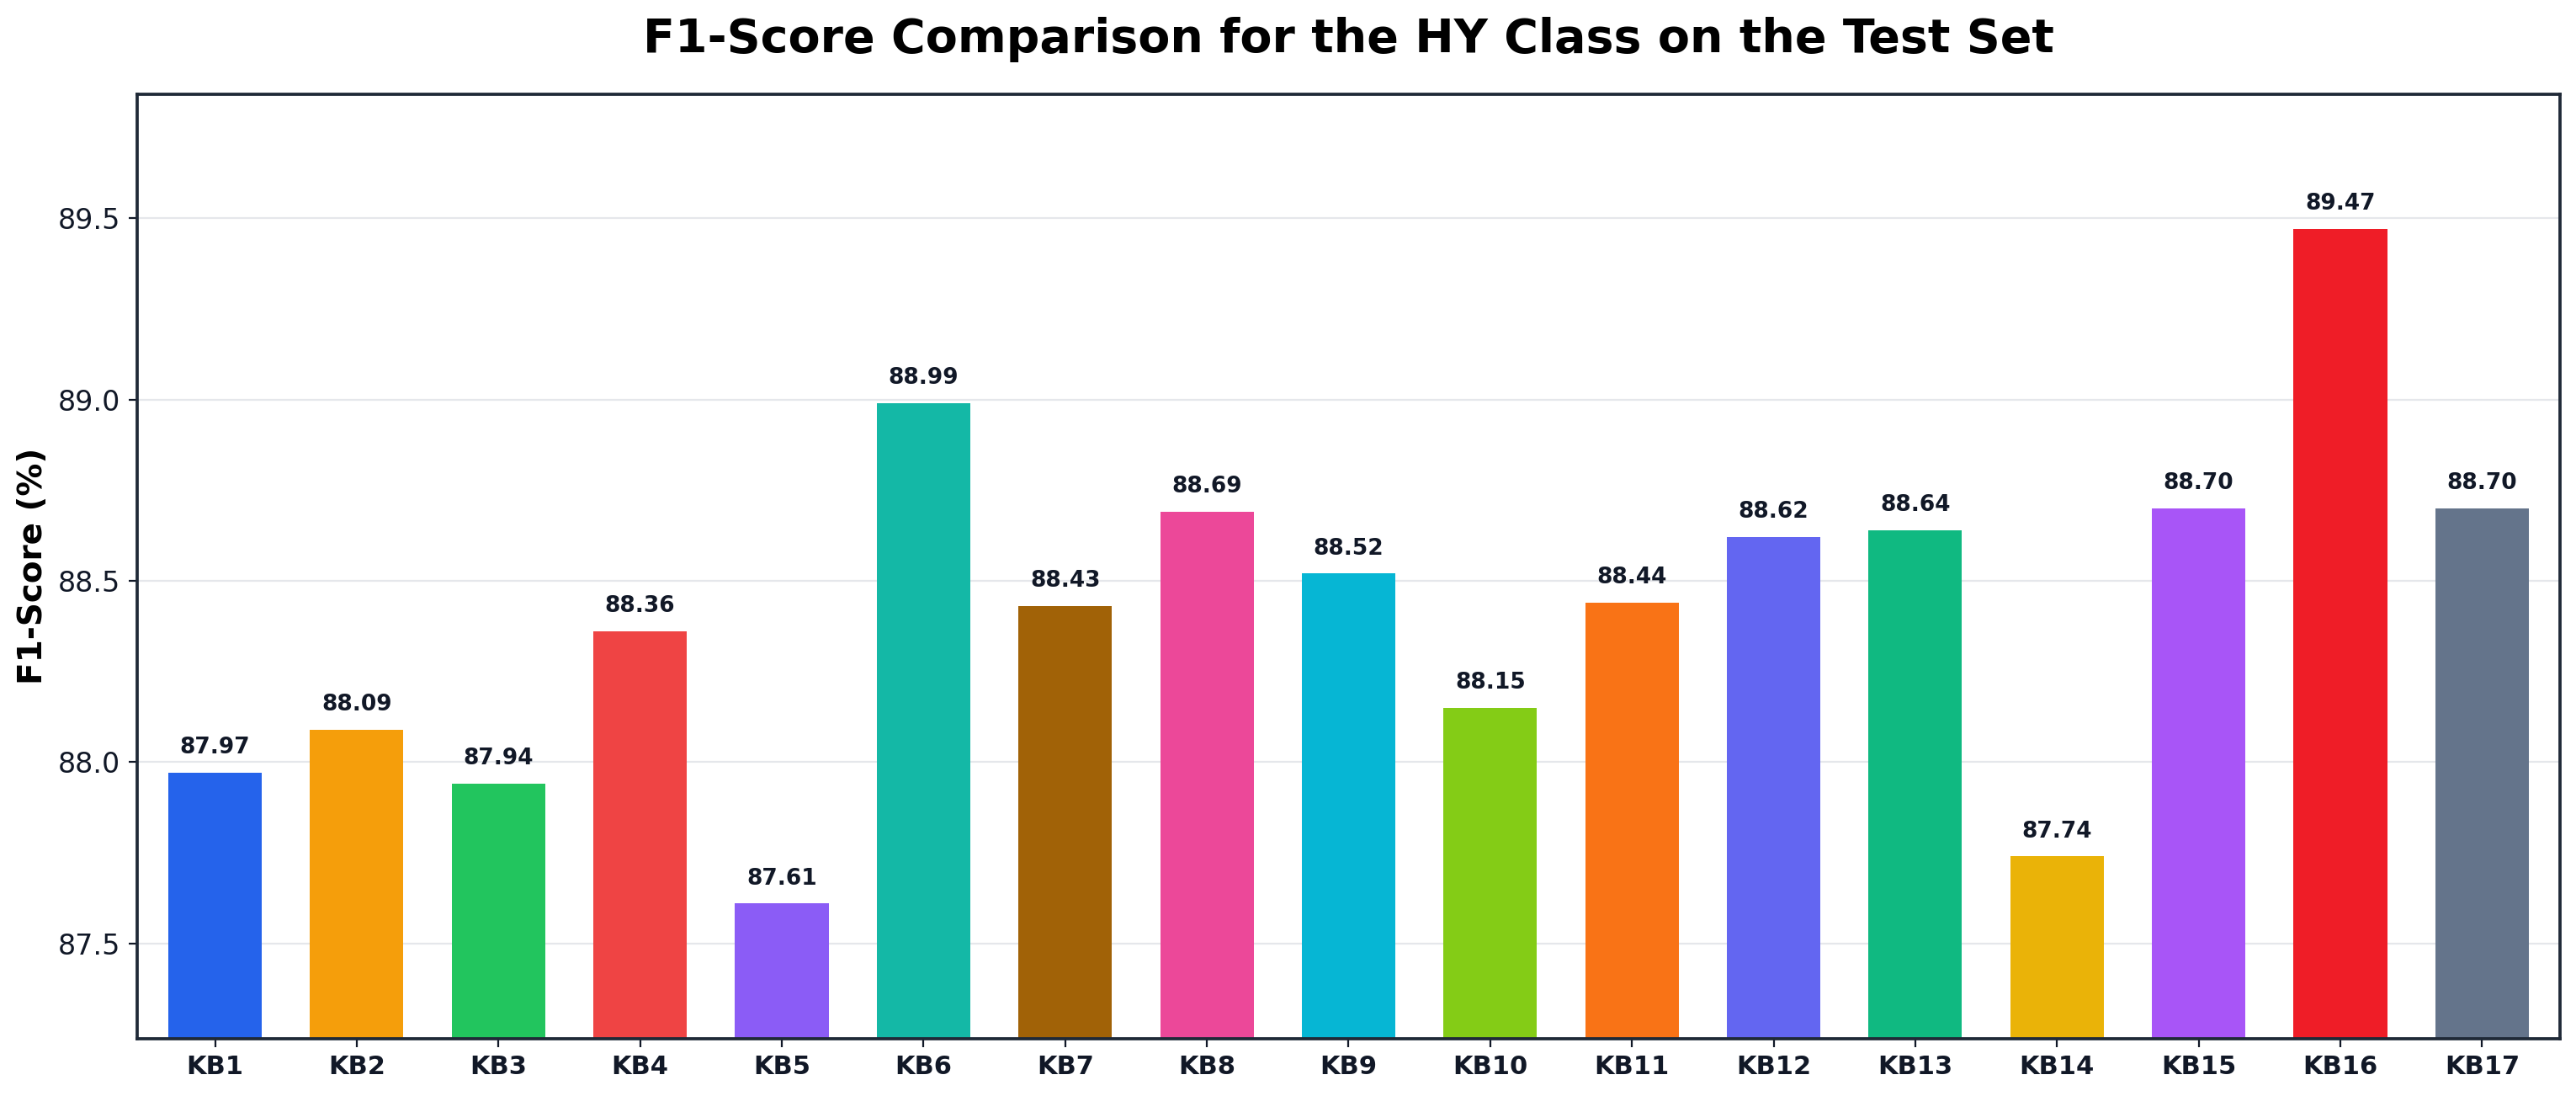
\includegraphics[width=\textwidth]{acc-loss/metric_f1_hy_test_english.png}
    \caption{F1-score of the HY class (High Yield)}
    \label{fig:F1-Score_hy}
\end{subfigure}
\end{figure}

\begin{figure}[H]
\ContinuedFloat
\centering
\begin{subfigure}{\fairfigurewidth}
    \centering
    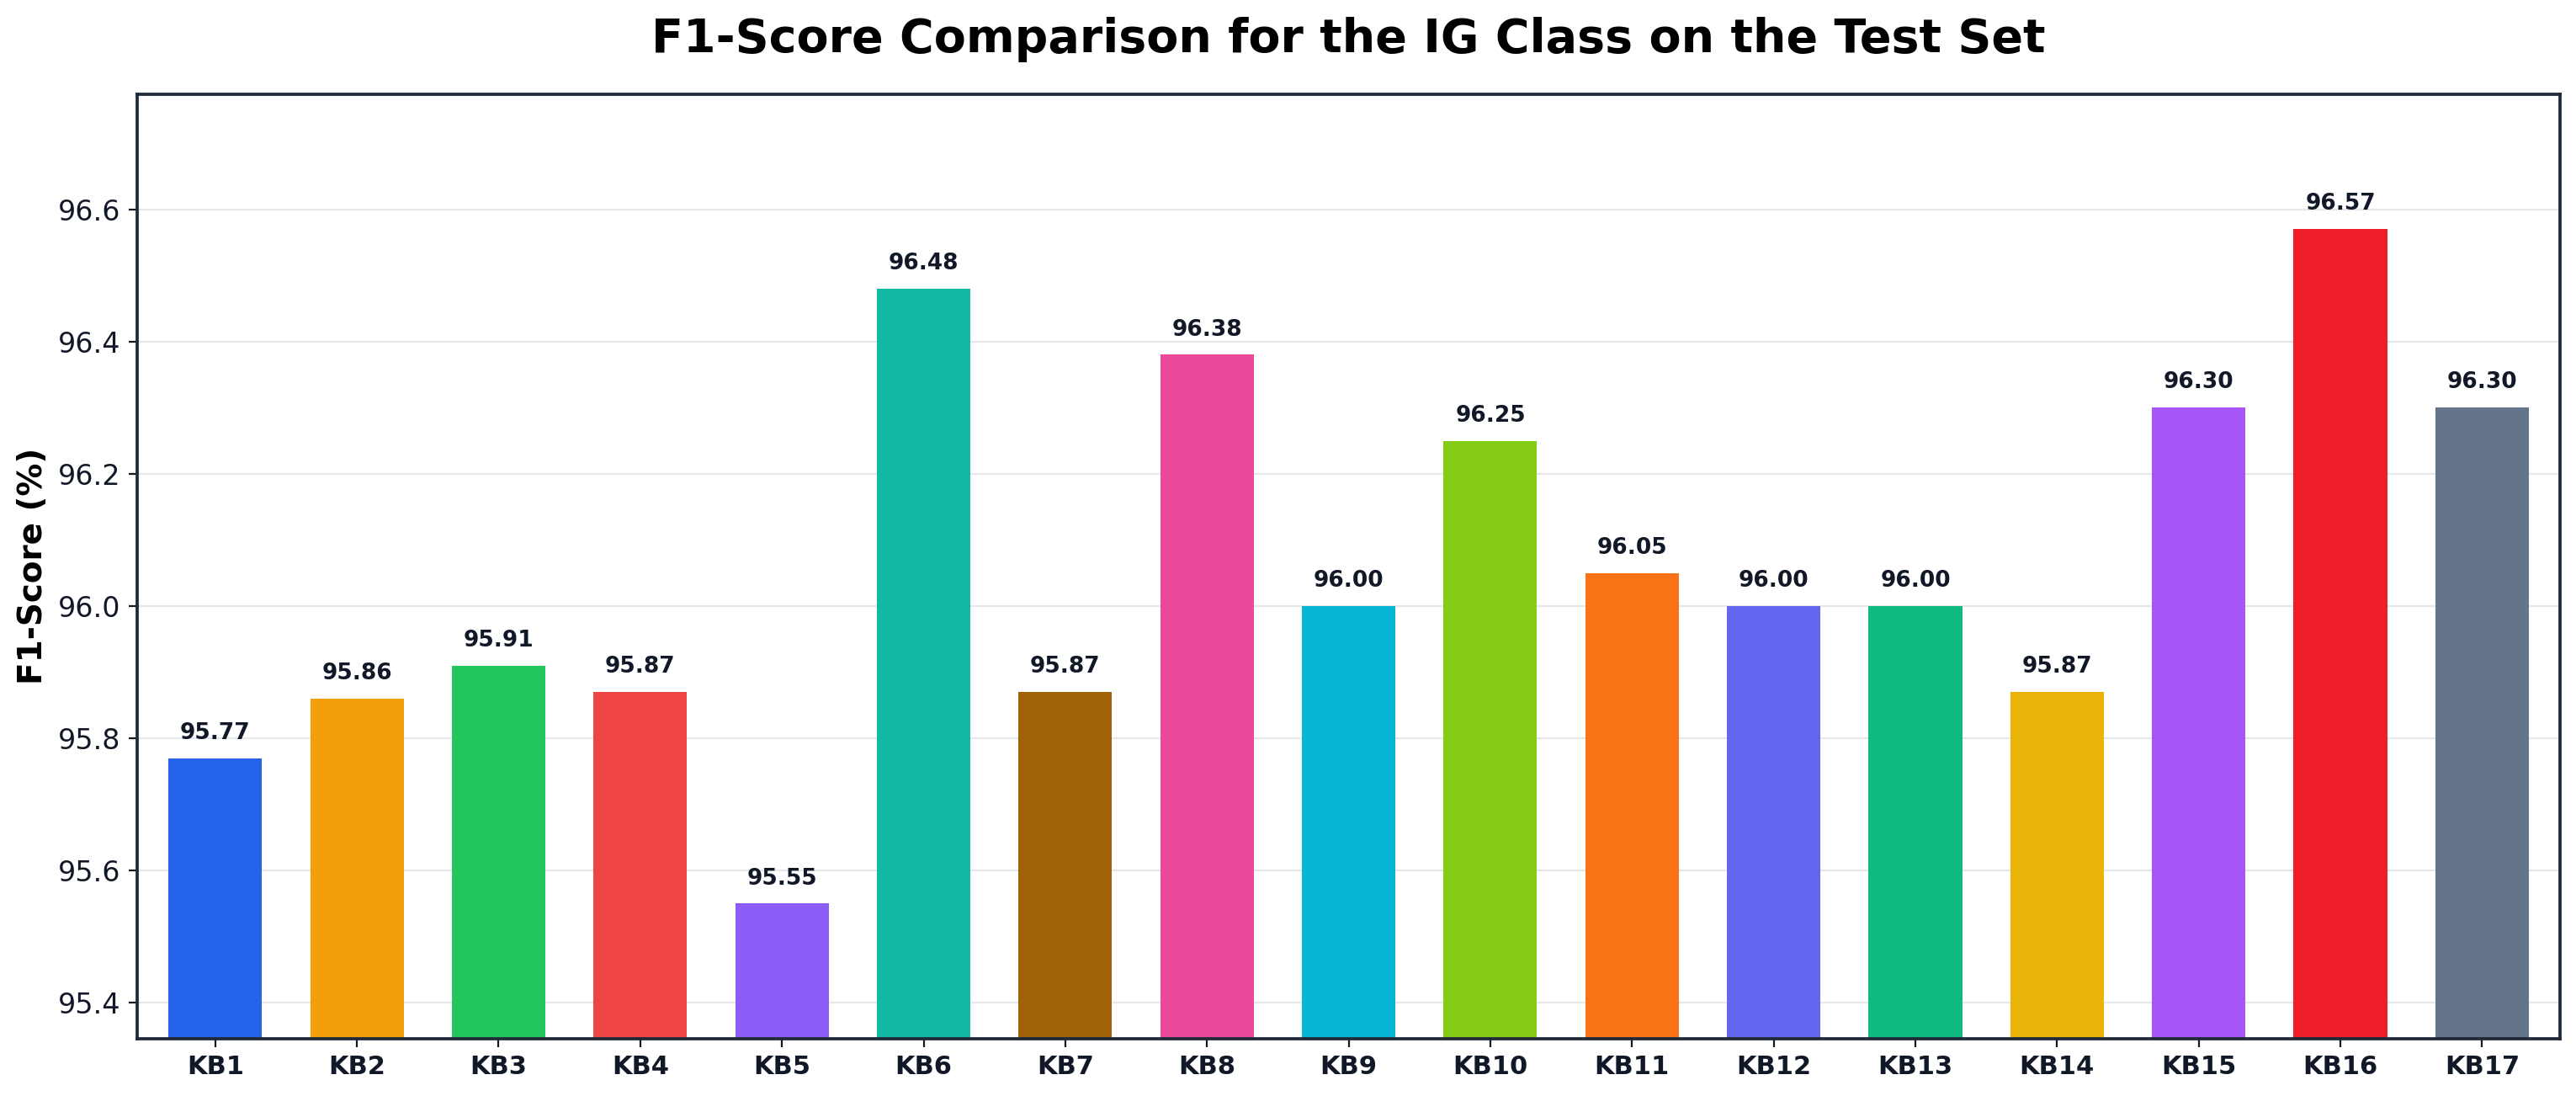
\includegraphics[width=\textwidth]{acc-loss/metric_f1_ig_test_english.png}
    \caption{F1-score of the IG class (Investment Grade)}
    \label{fig:F1-Score_ig}
\end{subfigure}
\caption{F1-score of the Distressed class (a), HY class (b), and IG class (c) on the test set}
\label{fig:F1-Score_classes}
\end{figure}
The F1-score of the Distressed class varies substantially across models. GraphSAGE achieves the highest value (63.25\%), FR-TTLPXL reaches 58.00\%, whereas PatchTST reaches 30.00\%. For the HY class, F1-score ranges from 87.61\% to 89.47\%; DMF obtains the highest value, followed by T-LSTM at 88.99\%. For the IG class, the models reach values from 95.55\% to 96.57\%, with DMF achieving the highest value. Therefore, DMF performs well on the two majority classes, whereas GraphSAGE is more suitable when the priority is to detect the Distressed class.

\subsubsection{Confusion matrix}

\begingroup
\renewcommand{\arraystretch}{1.2}
\setlength{\tabcolsep}{4pt}
\begin{longtable}{>{\centering\arraybackslash}m{0.31\textwidth}
                   >{\centering\arraybackslash}m{0.31\textwidth}
                   >{\centering\arraybackslash}m{0.31\textwidth}}
\caption{Confusion matrices of the scenarios on the test set}
\label{tab:confusion_matrices}\\

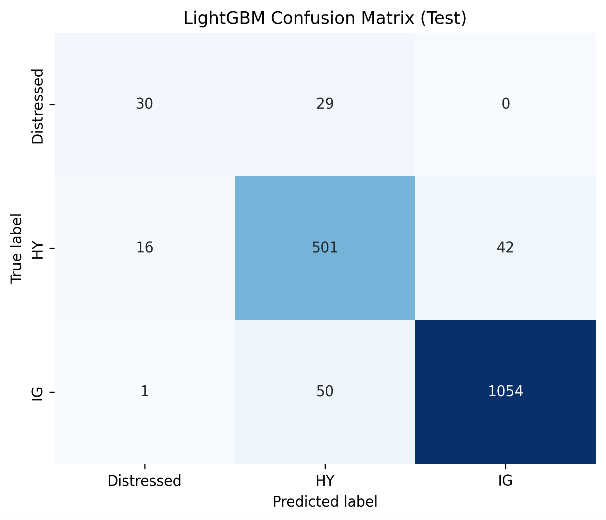
\includegraphics[width=0.95\linewidth]{acc-loss/confusion_lightgbm.png} &
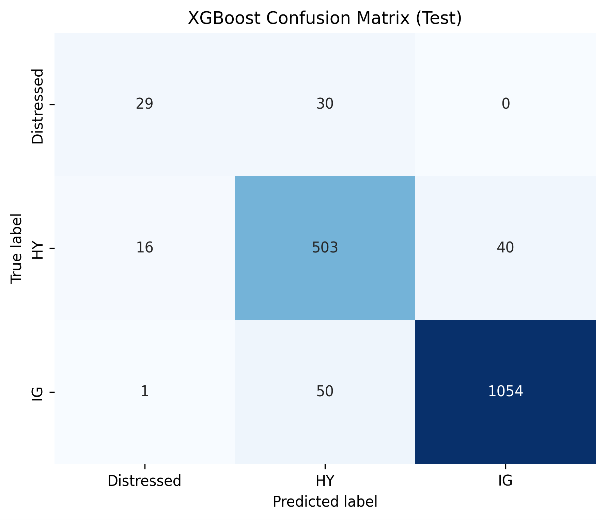
\includegraphics[width=0.95\linewidth]{acc-loss/confusion_xgboost.png} &
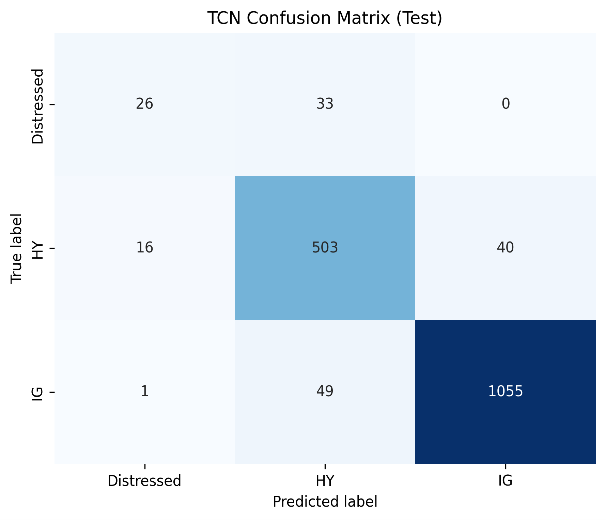
\includegraphics[width=0.95\linewidth]{acc-loss/confusion_tcn.png} \\

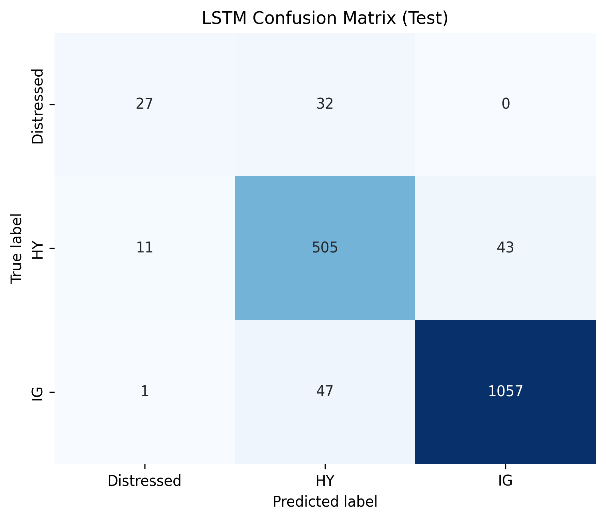
\includegraphics[width=0.95\linewidth]{acc-loss/confusion_lstm.png} &
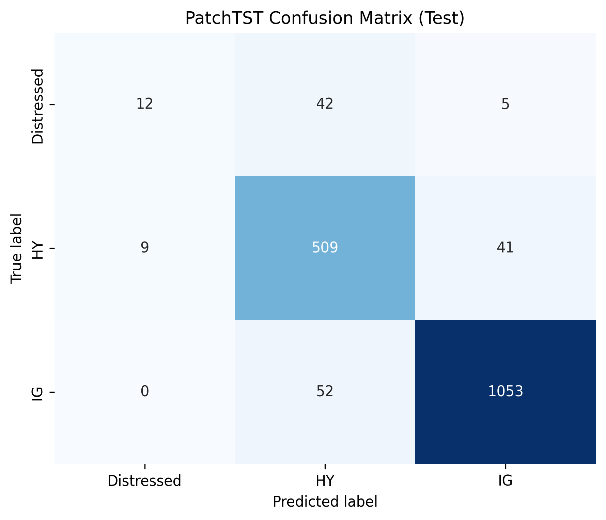
\includegraphics[width=0.95\linewidth]{acc-loss/confusion_patchtst.png} &
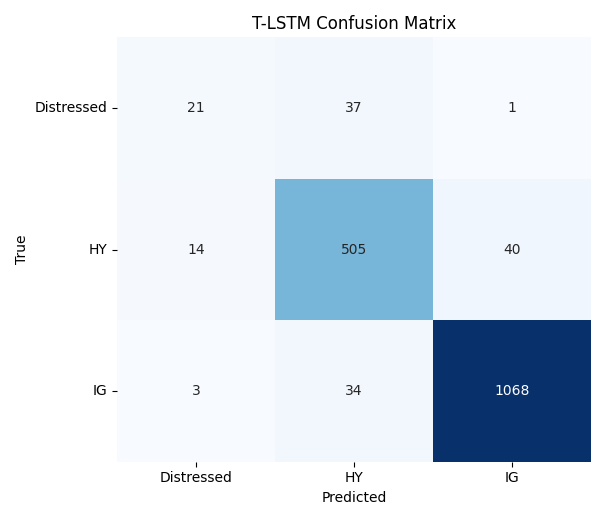
\includegraphics[width=0.95\linewidth]{acc-loss/confusion_tlstm.png} \\

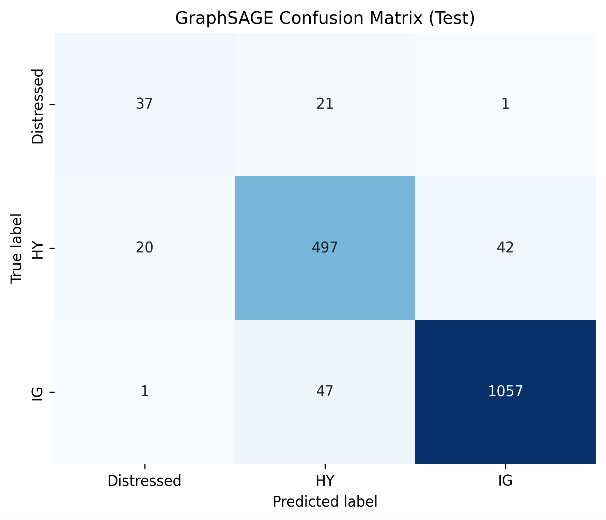
\includegraphics[width=0.95\linewidth]{acc-loss/confusion_graphsage.png} &
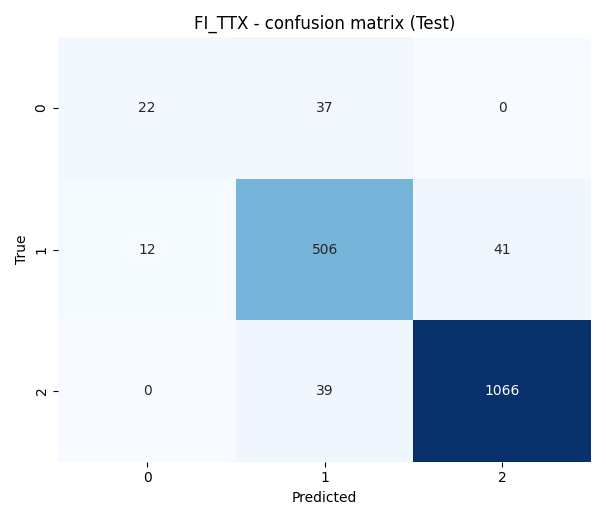
\includegraphics[width=0.95\linewidth]{acc-loss/confusion_fi_ttx.png} &
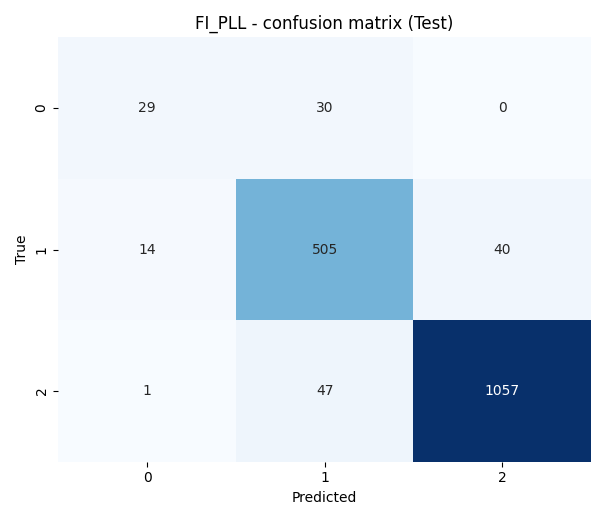
\includegraphics[width=0.95\linewidth]{acc-loss/confusion_fi_pll.png} \\

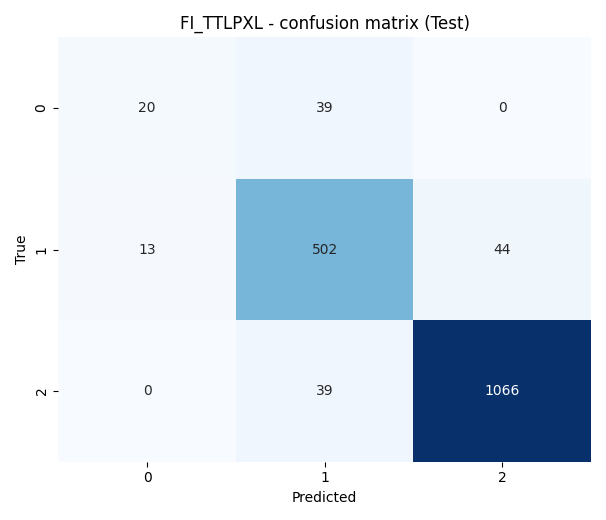
\includegraphics[width=0.95\linewidth]{acc-loss/confusion_fi_ttlpxl.png} &
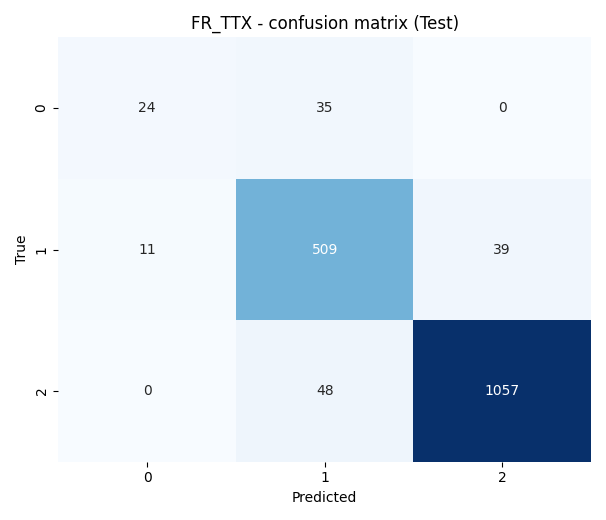
\includegraphics[width=0.95\linewidth]{acc-loss/confusion_fr_ttx.png} &
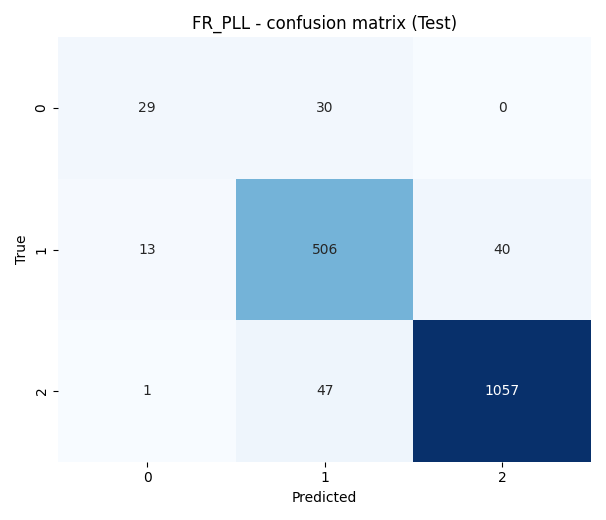
\includegraphics[width=0.95\linewidth]{acc-loss/confusion_fr_pll.png} \\

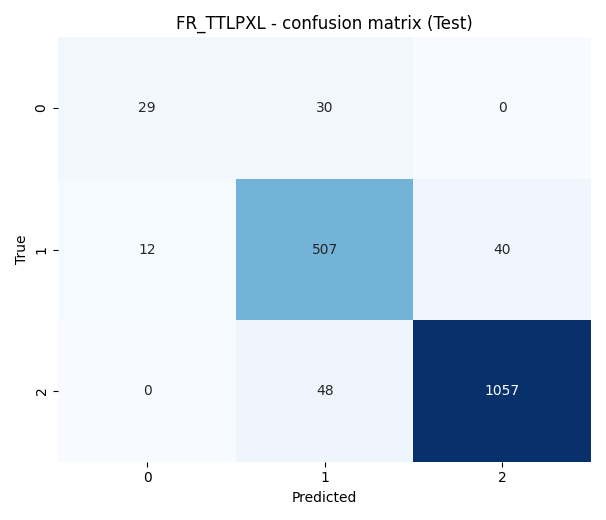
\includegraphics[width=0.95\linewidth]{acc-loss/confusion_fr_ttlpxl.png} &
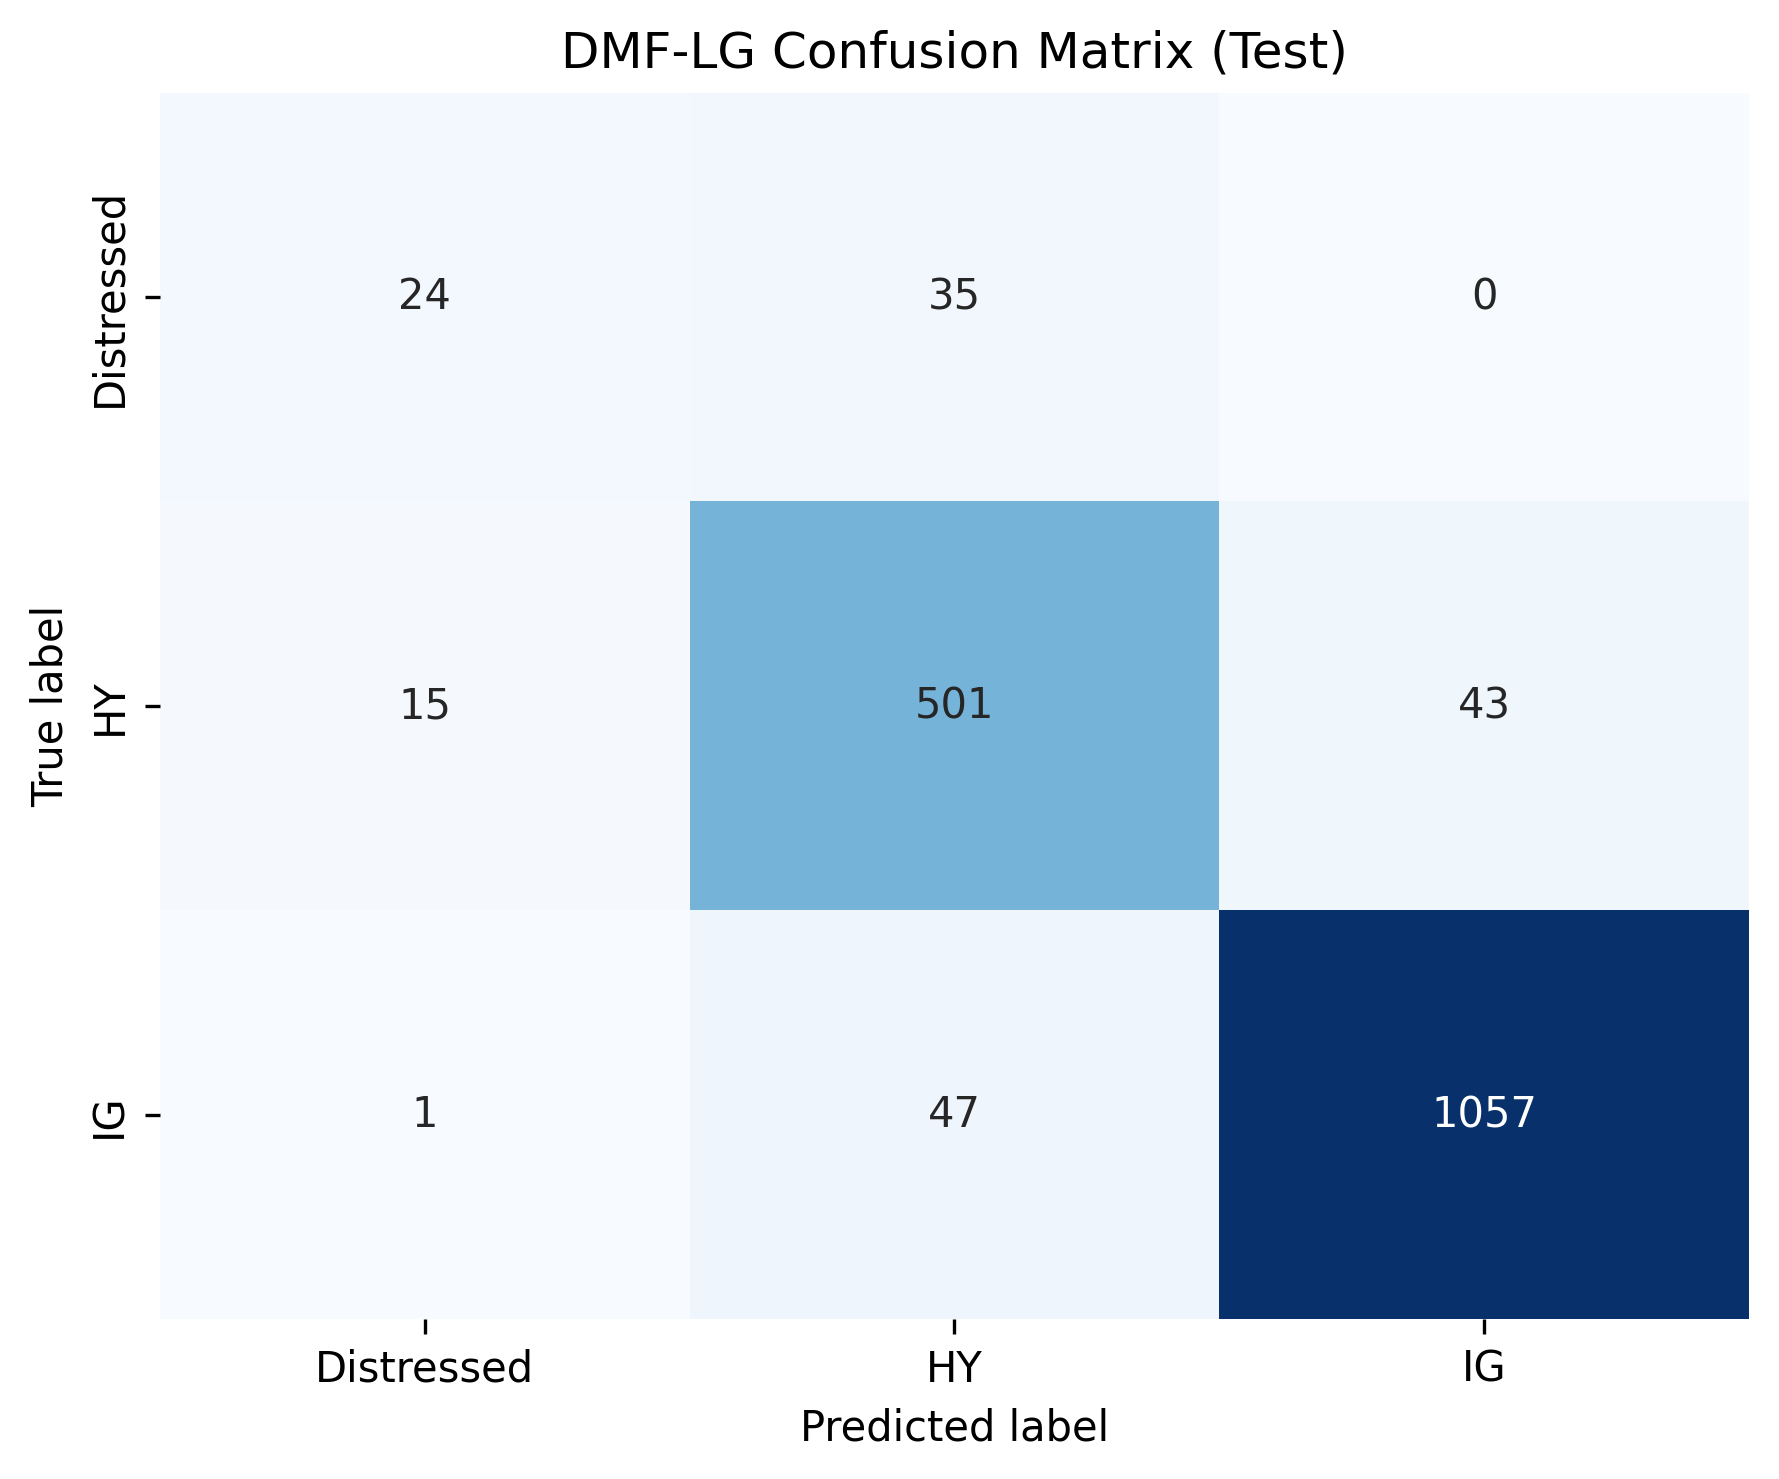
\includegraphics[width=0.95\linewidth]{acc-loss/confusion_dmf_lstm_graphsage.png} & \\
\end{longtable}
\endgroup

The confusion matrices show that IG is identified most consistently, while Distressed is often misclassified as HY. GraphSAGE correctly predicts 37 Distressed samples, the highest number among individual models. T-LSTM correctly predicts 1,068 IG samples. DMF/DCS correctly predicts 510 HY samples and 1,071 IG samples, but its detection of Distressed is weaker than that of GraphSAGE. This result is consistent with class-level Recall and indicates a trade-off between overall performance and the ability to detect the high-risk group.

\subsubsection{AUC-ROC of the scenarios}

\begin{figure}[H]
\centering
\setupfairsubfigures
\begin{subfigure}{\fairfigurewidth}
    \centering
    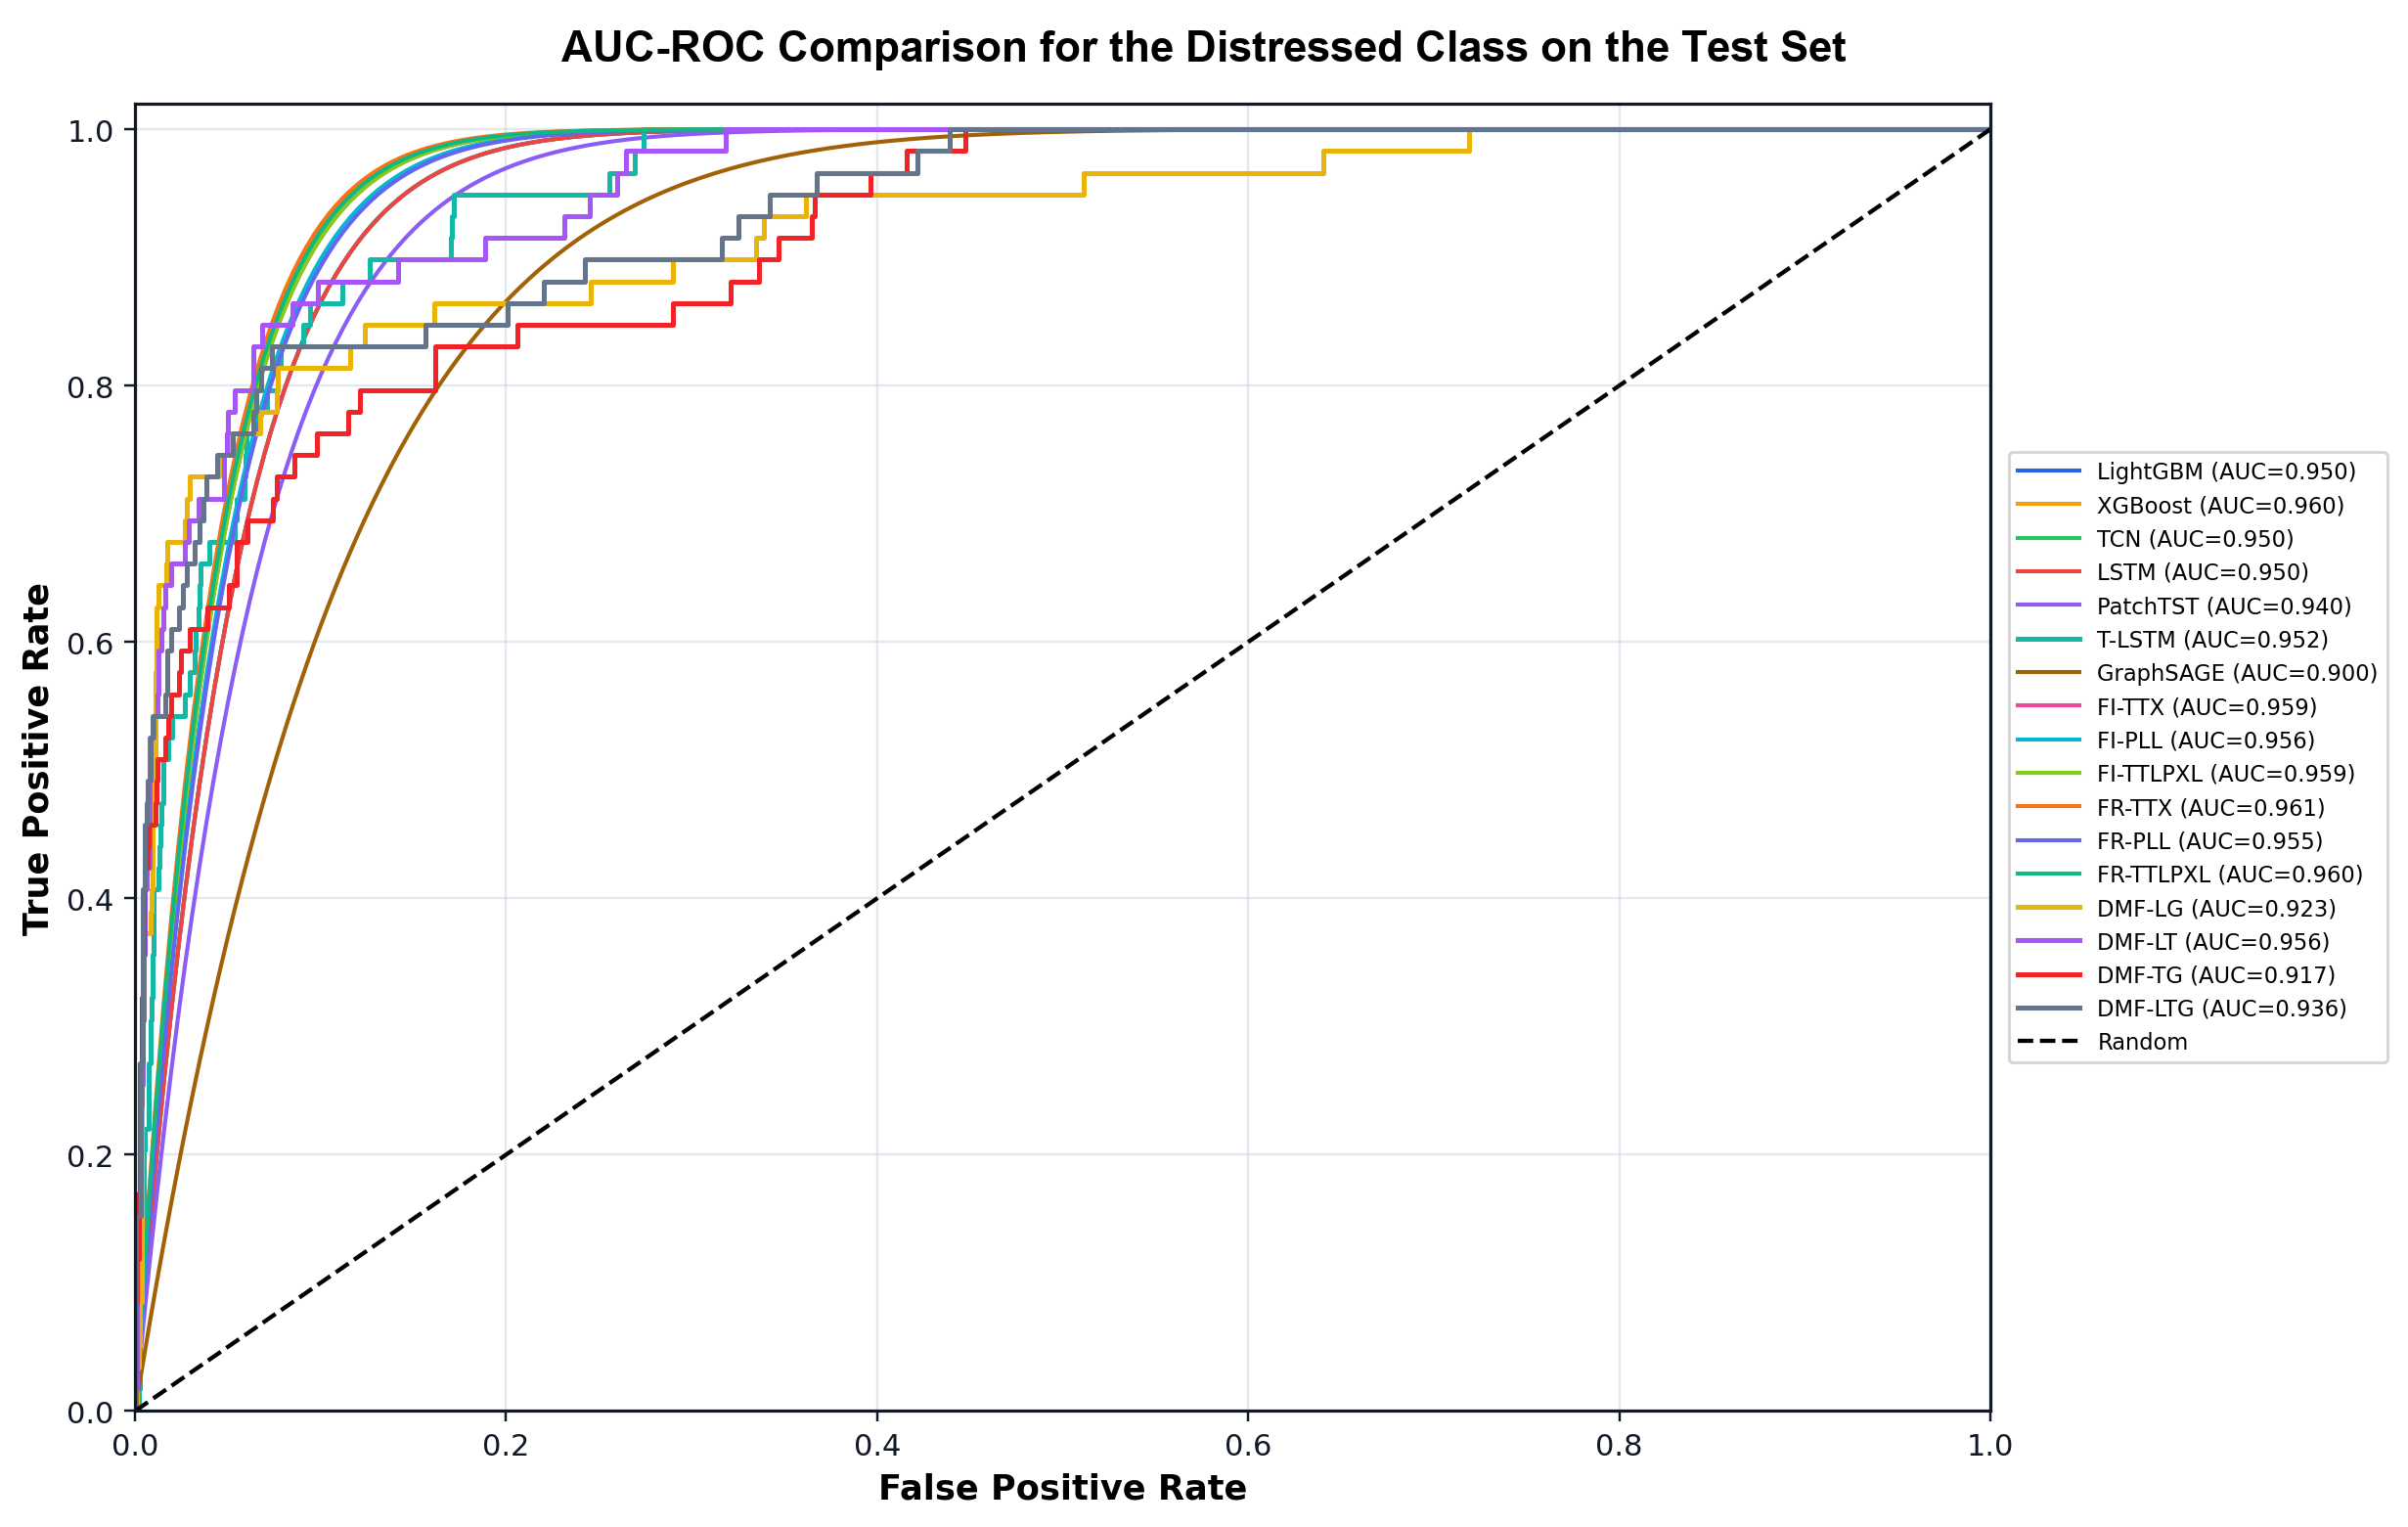
\includegraphics[width=\textwidth]{acc-loss/roc_distressed_17_models_english.png}
    \caption{ROC curve for the Distressed class}
    \label{fig:AUC-ROC_distressed}
\end{subfigure}
\end{figure}

\begin{figure}[H]
\ContinuedFloat
\centering
\begin{subfigure}{\fairfigurewidth}
    \centering
    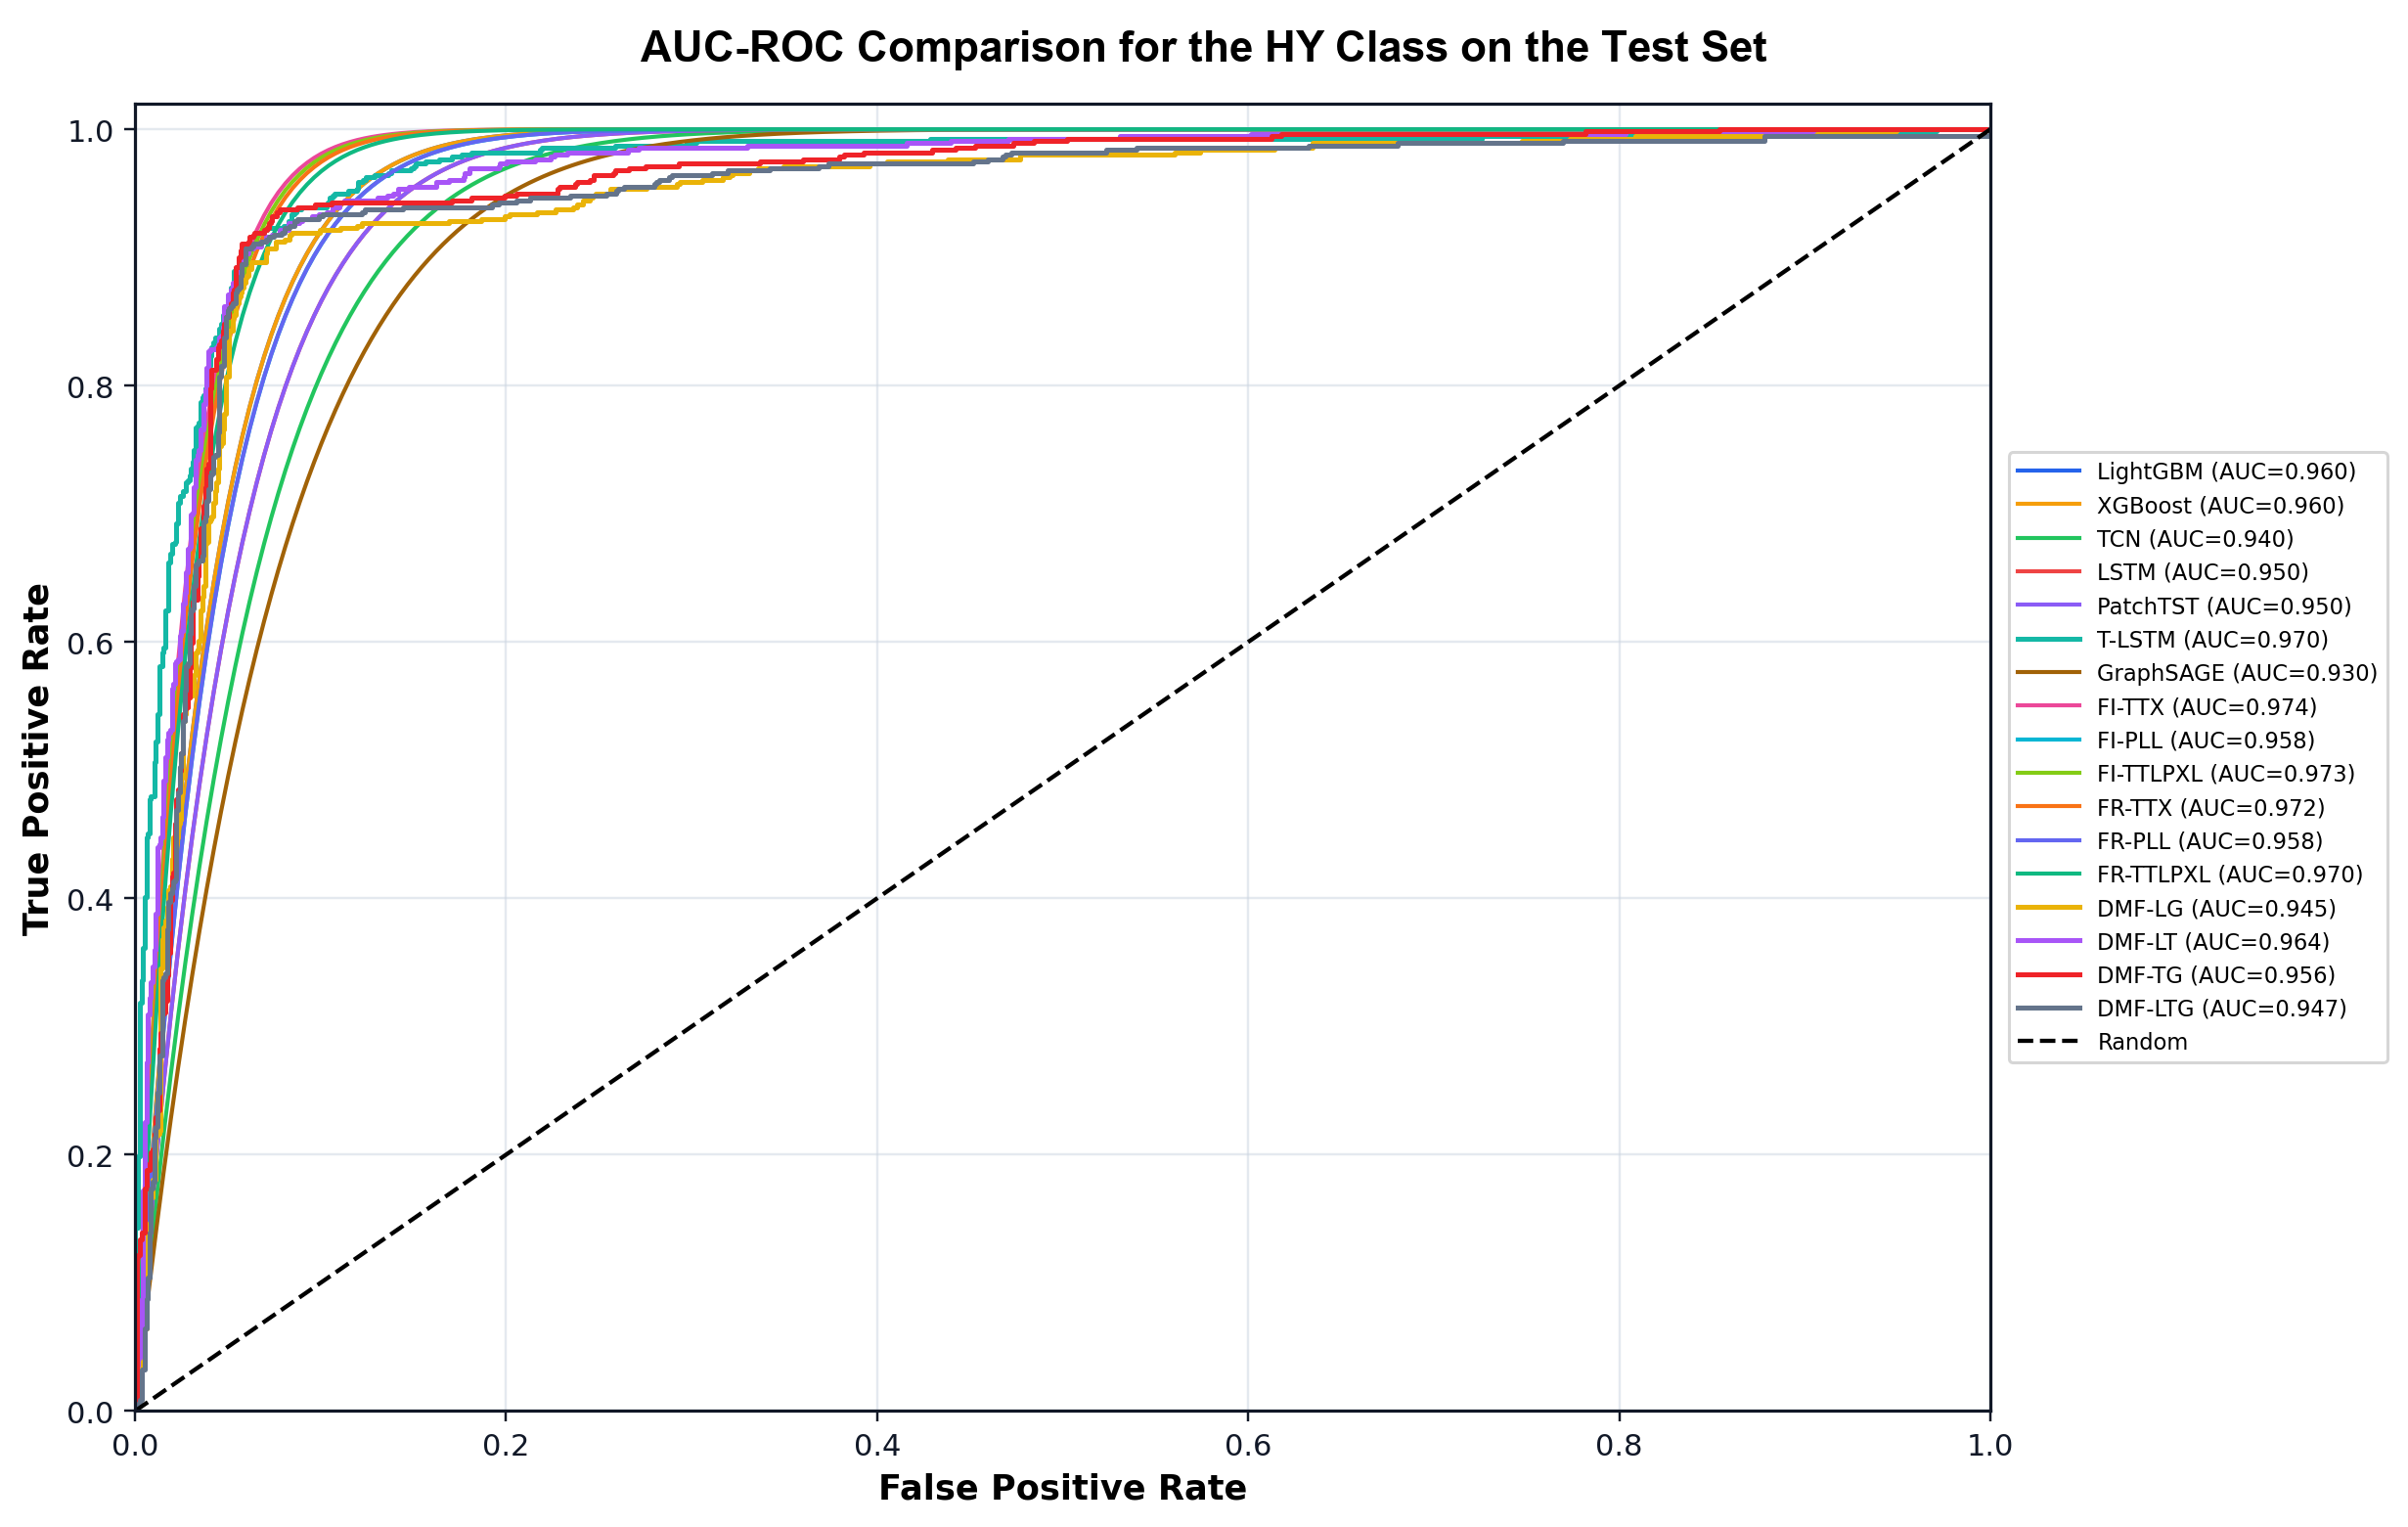
\includegraphics[width=\textwidth]{acc-loss/roc_hy_17_models_english.png}
    \caption{ROC curve for the HY class (High Yield)}
    \label{fig:AUC-ROC_hy}
\end{subfigure}
\end{figure}

\begin{figure}[H]
\ContinuedFloat
\centering
\begin{subfigure}{\fairfigurewidth}
    \centering
    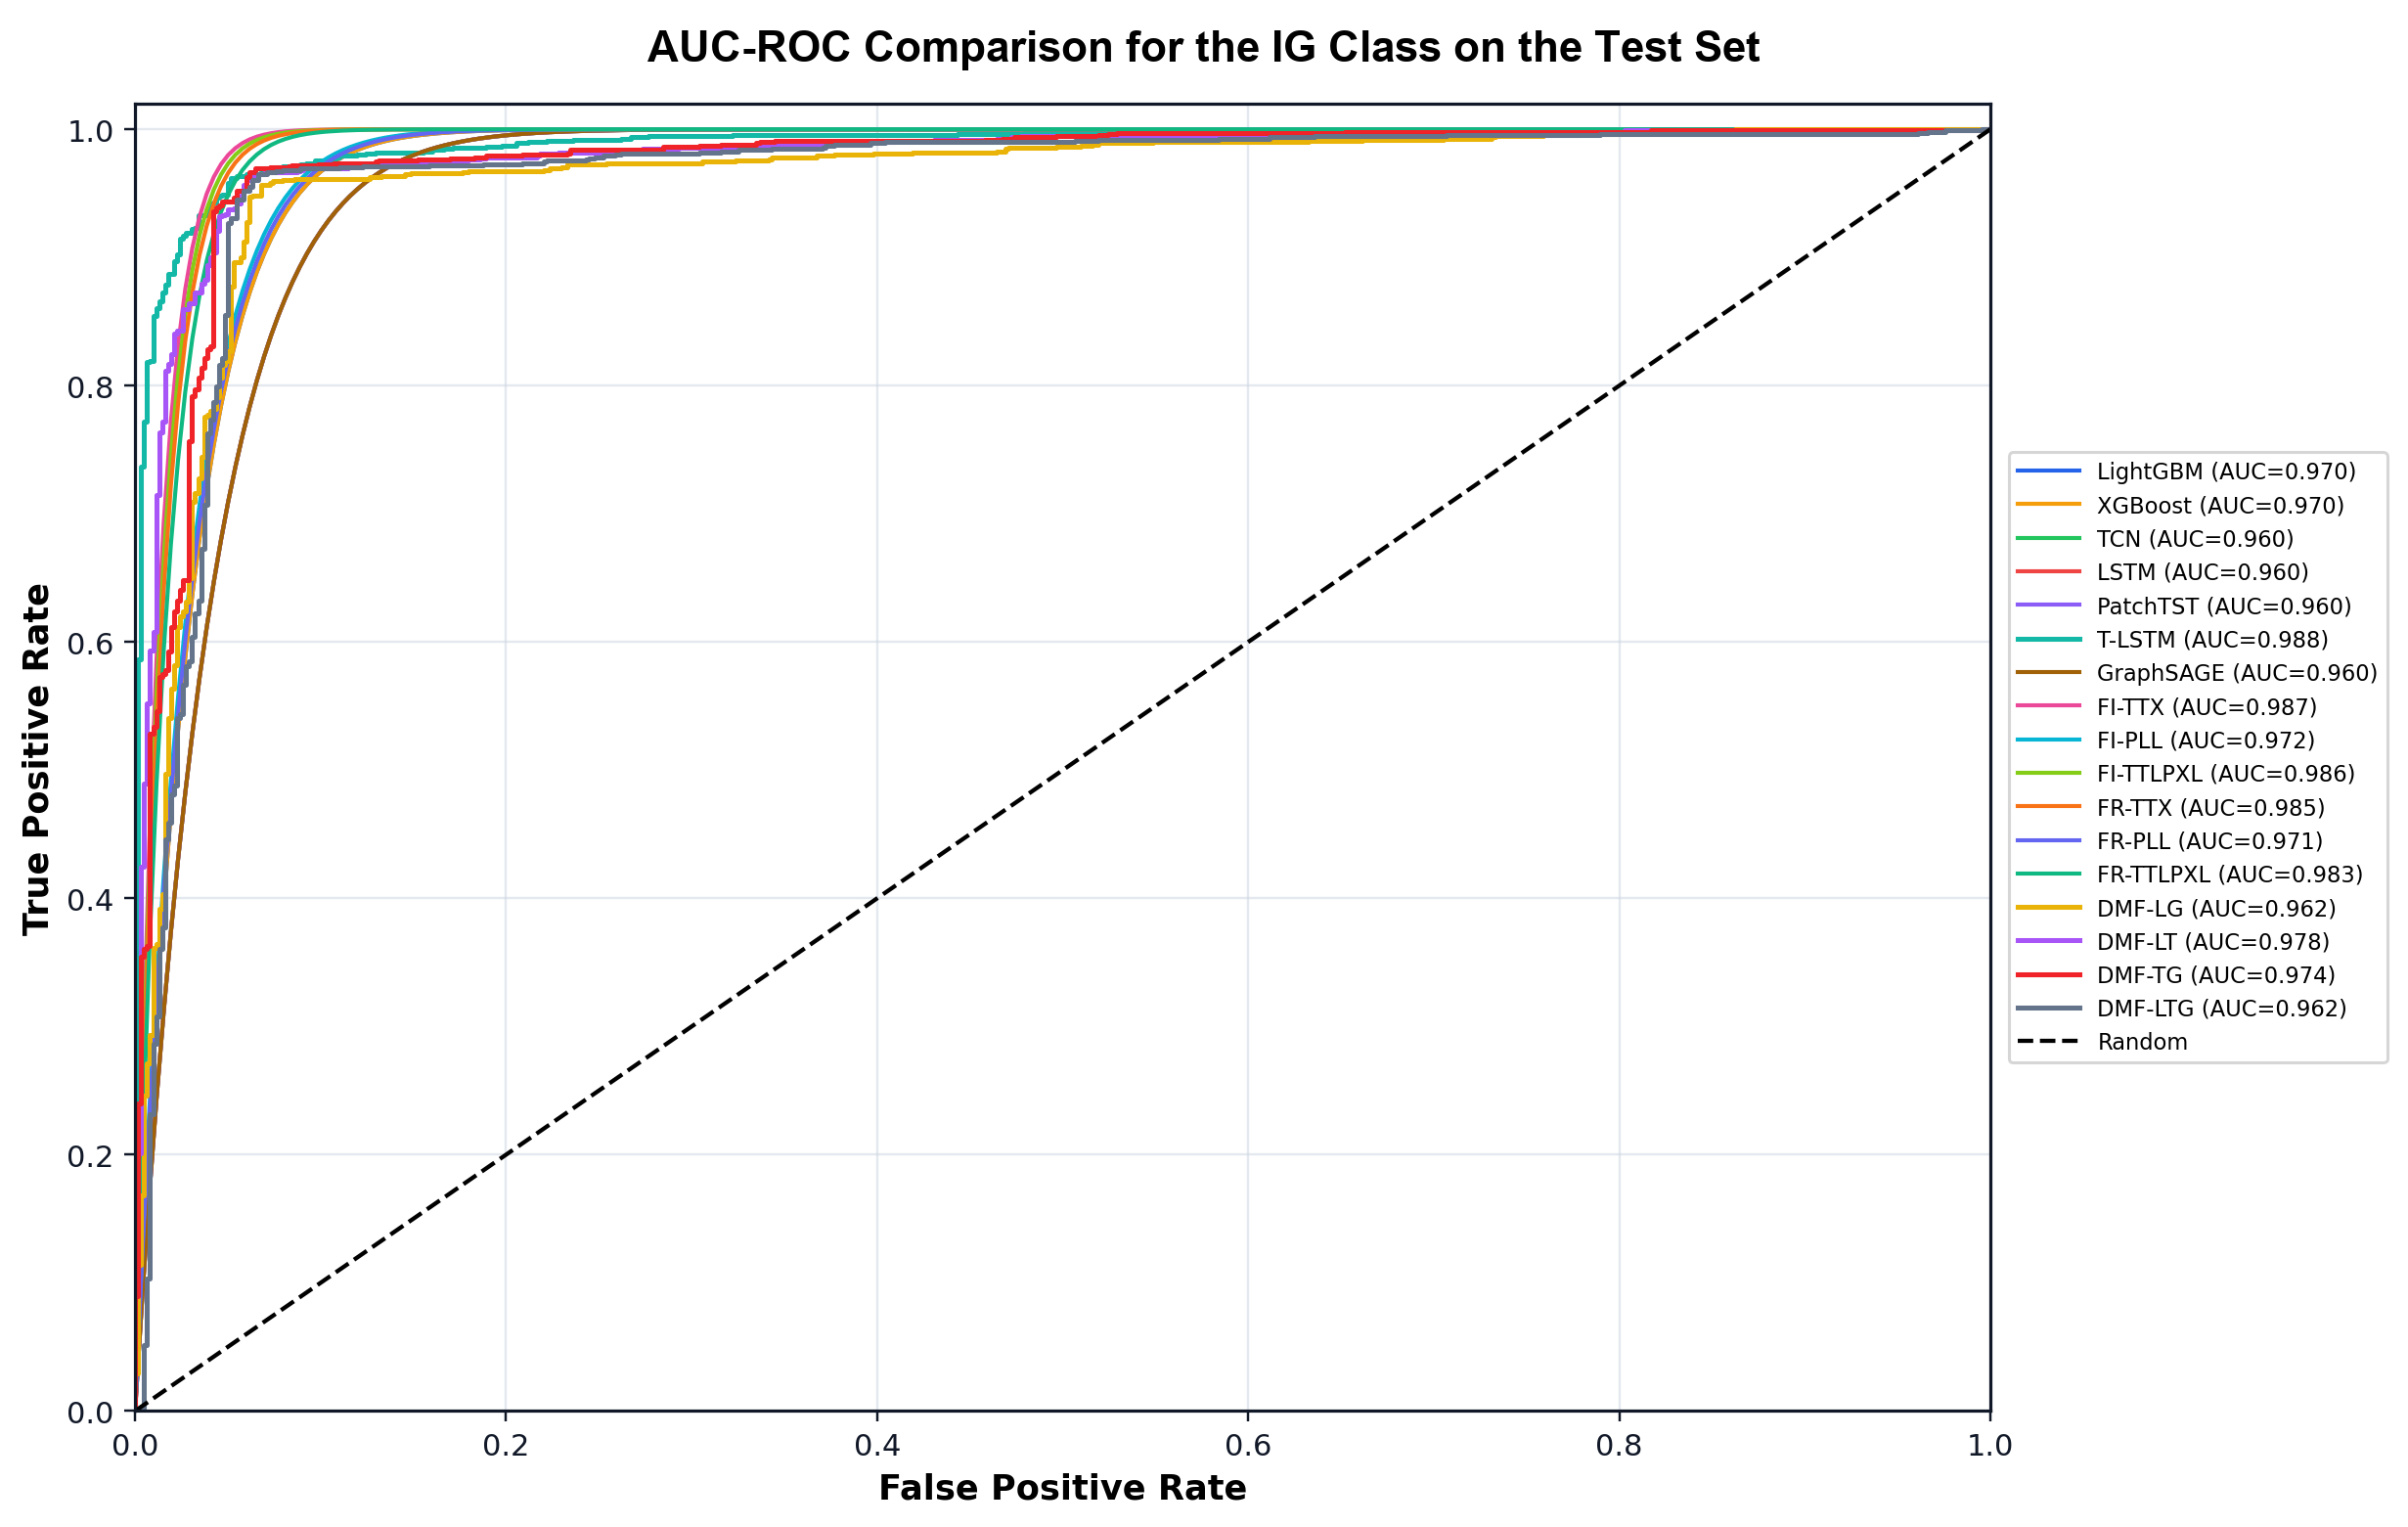
\includegraphics[width=\textwidth]{acc-loss/roc_ig_17_models_english.png}
    \caption{ROC curve for the IG class (Investment Grade)}
    \label{fig:AUC-ROC_ig}
\end{subfigure}
\caption{AUC-ROC of the Distressed class (a), HY class (b), and IG class (c) on the test set}
\label{fig:AUC-ROC_classes}
\end{figure}

AUC-ROC reaches high values for all three classes, but the leading model differs by class. FR-TTX obtains the highest AUC for Distressed (96.1\%); FI-TTX obtains the highest value for HY (97.4\%); and T-LSTM obtains the highest value for IG (98.8\%). DMF has the highest overall Accuracy but does not lead the AUC for each individual class. Therefore, model selection depends on whether the priority is overall performance or the ability to distinguish a specific risk group.

\subsubsection{Testing time}
\begin{figure}[H]
    \centering
    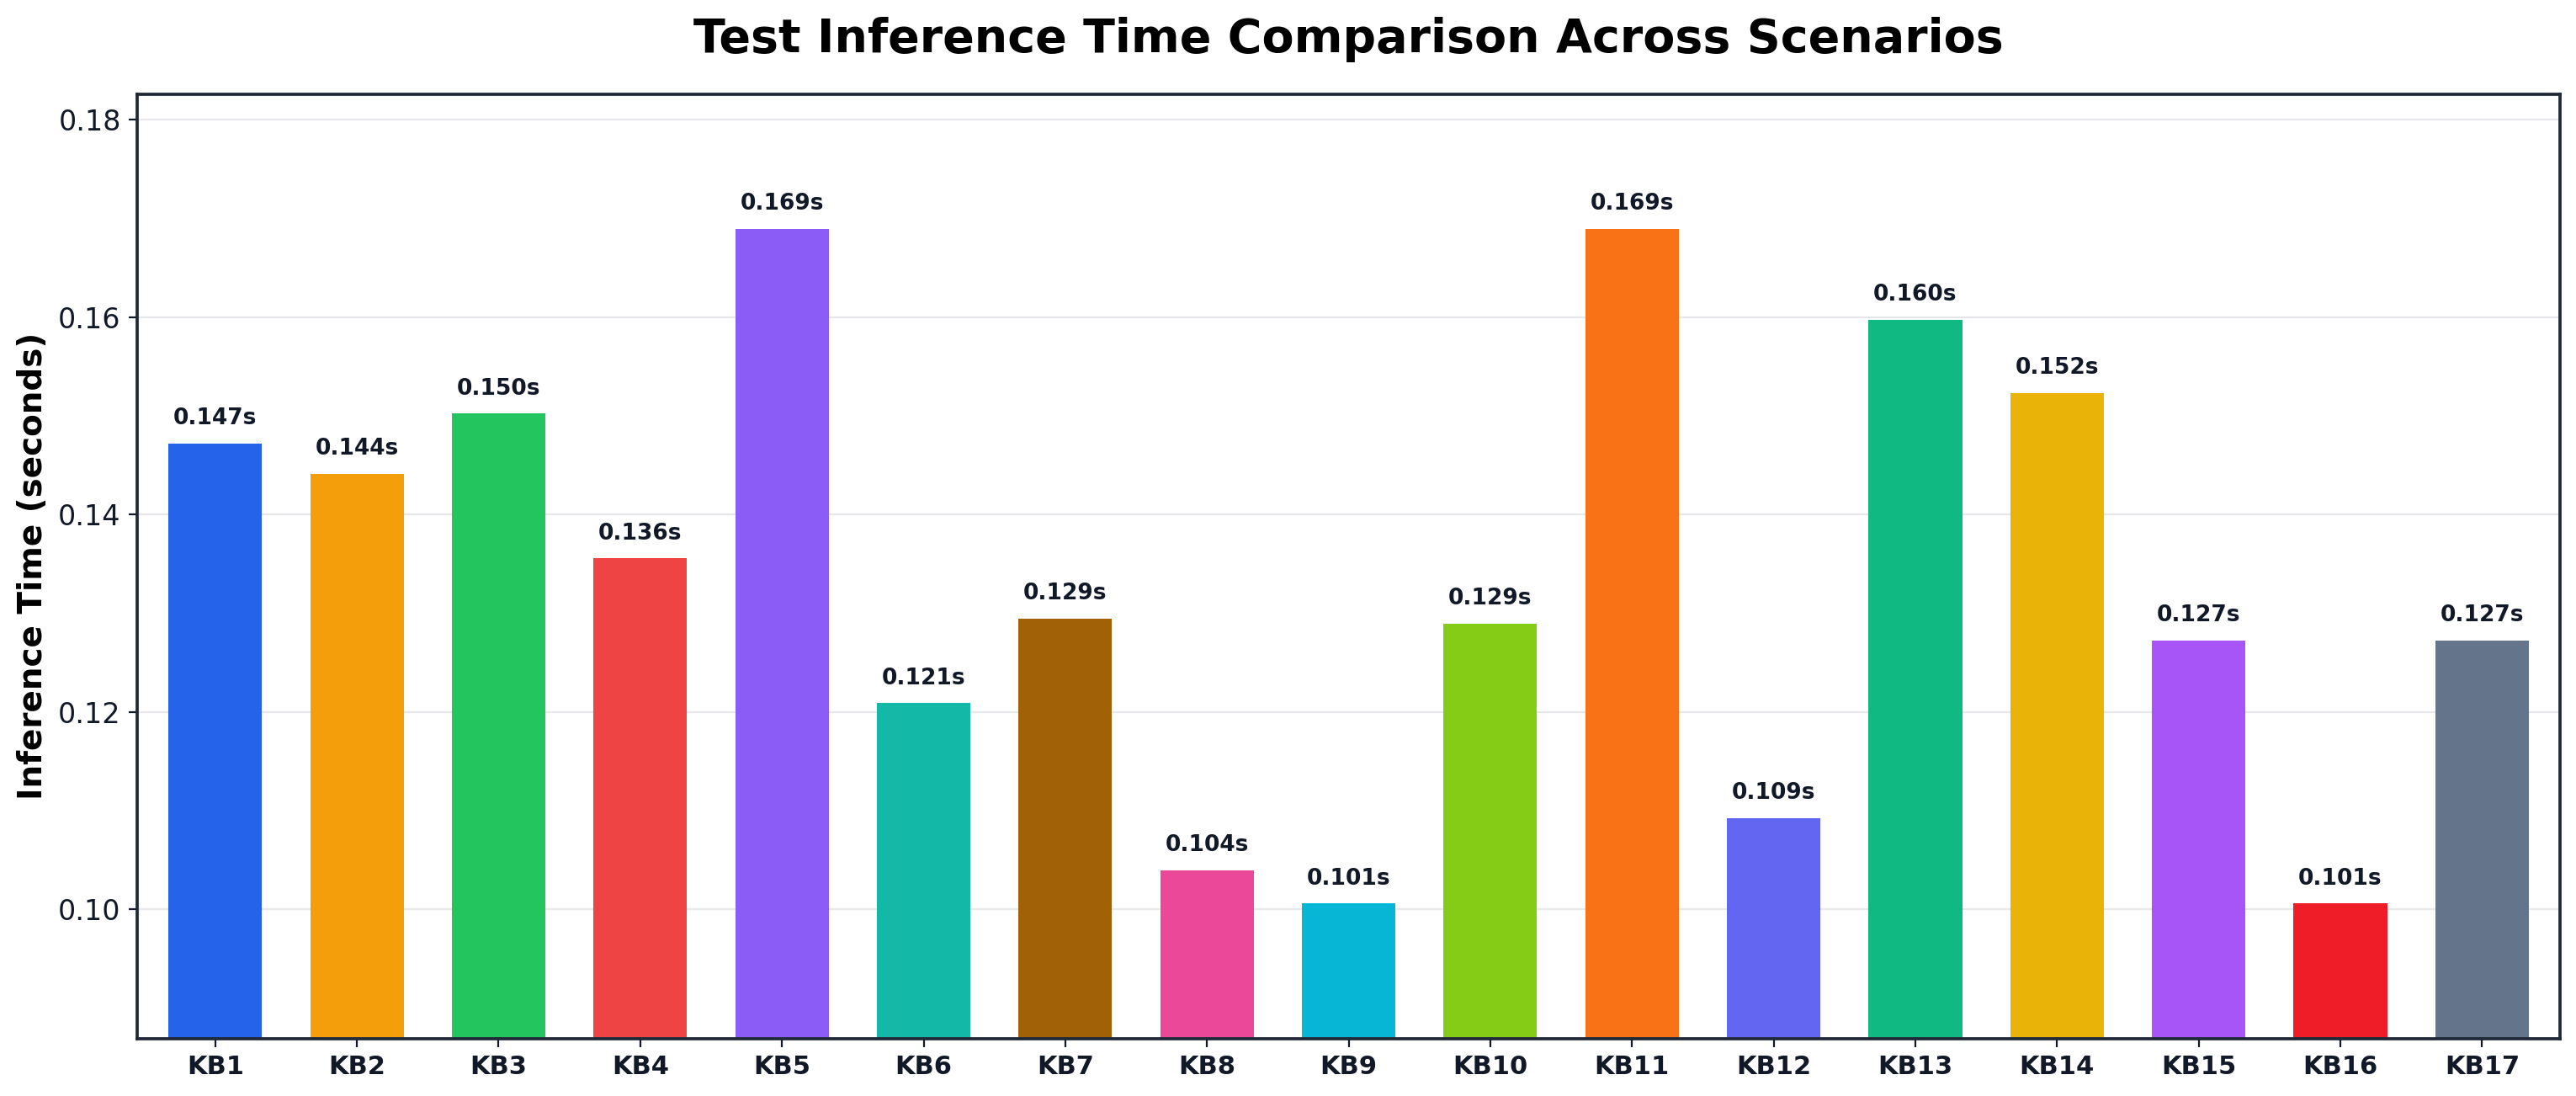
\includegraphics[width=\fairfigurewidth]{acc-loss/metric_inference_time_test_scenarios_english.png}
    \caption{Testing time of the scenarios}
\end{figure}

Testing time ranges from 0.101 to 0.169 seconds in the experimental environment. FI-PLL and DMF have the lowest time (0.101 seconds), whereas PatchTST and FR-TTX have the highest time (0.169 seconds). The absolute difference among scenarios is 0.068 seconds. These figures indicate low inference cost on the current test set, but they are not sufficient to conclude performance under large-scale deployment or on different infrastructure.

\subsubsection{XAI explanation results}
\paragraph{GradientSHAP}
GradientSHAP is used to measure the contribution of each financial ratio to the model's prediction probability. The method is applied directly to the trained model without using a surrogate model. Sequential financial features are reduced by taking the mean value over the time window; GradientSHAP then estimates each variable's contribution through multiple samples between the explained sample and the background set.

\begingroup
\centering
\renewcommand{\arraystretch}{0.85}
\setlength{\tabcolsep}{2pt}
\begin{longtable}{>{\centering\arraybackslash}m{\fairfigurewidth}}
\caption{GradientSHAP results of the scenarios on the test set}
\label{tab:gradientshap_results}\\
\xairesultcell{GradientSHAP result of scenario 1}{acc-loss/xai_shap_lightgbm.png} \\
\xairesultcell{GradientSHAP result of scenario 2}{acc-loss/xai_shap_xgboost.png} \\
\xairesultcell{GradientSHAP result of scenario 3}{acc-loss/xai_shap_tcn.png} \\
\xairesultcell{GradientSHAP result of scenario 4}{acc-loss/xai_shap_lstm.png} \\
\xairesultcell{GradientSHAP result of scenario 5}{acc-loss/xai_shap_patchtst.png} \\
\xairesultcell{GradientSHAP result of scenario 6}{acc-loss/xai_shap_tlstm.png} \\
\xairesultcell{GradientSHAP result of scenario 7}{acc-loss/xai_shap_graphsage.png} \\
\xairesultcell{GradientSHAP result of scenario 8}{acc-loss/xai_shap_fi_ttx.png} \\
\xairesultcell{GradientSHAP result of scenario 9}{acc-loss/xai_shap_fi_pll.png} \\
\xairesultcell{GradientSHAP result of scenario 10}{acc-loss/xai_shap_fi_ttlpxl.png} \\
\xairesultcell{GradientSHAP result of scenario 11}{acc-loss/xai_shap_fr_ttx.png} \\
\xairesultcell{GradientSHAP result of scenario 12}{acc-loss/xai_shap_fr_pll.png} \\
\xairesultcell{GradientSHAP result of scenario 13}{acc-loss/xai_shap_fr_ttlpxl.png} \\
\xairesultcell{GradientSHAP result of scenario 14}{acc-loss/xai_shap_dmf_lstm_graphsage.png} \\
\end{longtable}
\endgroup

GradientSHAP records large contributions from features related to profitability, leverage, and liquidity. Pretax Profit Margin and Operating Profit Margin frequently appear among the features with high contributions. Debt-to-Equity Ratio and Current Ratio are also used by many models to distinguish risk groups. T-LSTM and GraphSAGE also assign contributions to ROA, ROE, Asset Turnover, and cash-flow variables. For DMF/DCS, the prominent features include Pretax Profit Margin, Operating Profit Margin, Debt-to-Equity Ratio, and Current Ratio. These results are consistent with the commonly recognized roles of profitability, leverage, and liquidity in credit analysis; they support the interpretation of model behavior but do not establish causal relationships.

\paragraph{LIME}
LIME is used as a local, model-agnostic explanation method. In this study, after the model produces a credit-rating result for a specific firm, LIME generates multiple perturbed data samples around the original sample by slightly changing the values of financial features. These perturbed samples are then fed into the trained model to observe changes in prediction probabilities. In the LIME charts, orange indicates features that increase the probability of the model predicting the class under consideration. Conversely, blue indicates features that decrease the probability of belonging to that class. The longer the bar, the greater the influence of the feature.

\begingroup
\centering
\renewcommand{\arraystretch}{0.85}
\setlength{\tabcolsep}{2pt}
\begin{longtable}{>{\centering\arraybackslash}m{\fairfigurewidth}}
\caption{LIME results of the scenarios on the test set}
\label{tab:lime_results}\\
\xairesultcell{LIME result of scenario 1}{acc-loss/xai_lime_lightgbm.png} \\
\xairesultcell{LIME result of scenario 2}{acc-loss/xai_lime_xgboost.png} \\
\xairesultcell{LIME result of scenario 3}{acc-loss/xai_lime_tcn.png} \\
\xairesultcell{LIME result of scenario 4}{acc-loss/xai_lime_lstm.png} \\
\xairesultcell{LIME result of scenario 5}{acc-loss/xai_lime_patchtst.png} \\
\xairesultcell{LIME result of scenario 6}{acc-loss/xai_lime_tlstm.png} \\
\xairesultcell{LIME result of scenario 7}{acc-loss/xai_lime_graphsage.png} \\
\xairesultcell{LIME result of scenario 8}{acc-loss/xai_lime_fi_ttx.png} \\
\xairesultcell{LIME result of scenario 9}{acc-loss/xai_lime_fi_pll.png} \\
\xairesultcell{LIME result of scenario 10}{acc-loss/xai_lime_fi_ttlpxl.png} \\
\xairesultcell{LIME result of scenario 11}{acc-loss/xai_lime_fr_ttx.png} \\
\xairesultcell{LIME result of scenario 12}{acc-loss/xai_lime_fr_pll.png} \\
\xairesultcell{LIME result of scenario 13}{acc-loss/xai_lime_fr_ttlpxl.png} \\
\xairesultcell{LIME result of scenario 14}{acc-loss/xai_lime_dmf_legacy.png} \\
\end{longtable}
\endgroup

GradientSHAP and LIME provide two complementary levels of interpretation. GradientSHAP describes feature contributions across multiple observations, whereas LIME locally approximates the model's behavior around a specific prediction. The two methods help trace financial indicators related to predictions, thereby supporting the transparency of the system. However, explanation results depend on the background samples, perturbation strategy, and configuration of each method.

\subsection{Comparison and discussion}

\begingroup
\centering
\setlength{\tabcolsep}{4pt}
\renewcommand{\arraystretch}{1.05}
\begin{longtable}{c l c c c c}
\caption{Comparison of scenarios on the test dataset}
\label{tab:test_scenarios_comparison}\\
\hline
\textbf{Scenario} & \textbf{Scenario name} & \textbf{Accuracy (\%)} & \textbf{Precision (\%)} & \textbf{Recall (\%)} & \textbf{F1-score (\%)} \\
\hline
\endfirsthead
\caption[]{Comparison of scenarios on the test dataset (continued)}\\
\hline
\textbf{Scenario} & \textbf{Scenario name} & \textbf{Accuracy (\%)} & \textbf{Precision (\%)} & \textbf{Recall (\%)} & \textbf{F1-score (\%)} \\
\hline
\endhead
\hline
\multicolumn{6}{r}{\fairsmallfont Continued on the next page}\\
\endfoot
\hline
\endlastfoot
1  & LightGBM   & 91.99 & 91.88 & 91.99 & 91.90 \\
2  & XGBoost    & 92.05 & 91.94 & 92.05 & 91.95 \\
3  & TCN        & 91.93 & 91.76 & 91.93 & 91.78 \\
4  & LSTM       & 92.22 & 92.05 & 92.22 & 92.04 \\
5  & PatchTST   & 91.35 & 90.79 & 91.35 & 90.73 \\
6  & T-LSTM     & 92.51 & 92.10 & 92.51 & 92.23 \\
7  & GraphSAGE  & 92.34 & 92.35 & 92.34 & 92.34 \\
8  & FI-TTX     & 92.51 & 92.18 & 92.51 & 92.21 \\
9  & FI-PLL     & 92.34 & 92.20 & 92.34 & 92.22 \\
10 & FI-TTLPXL  & 92.16 & 91.75 & 92.16 & 91.82 \\
11 & FR-TTX     & 92.28 & 92.09 & 92.28 & 92.04 \\
12 & FR-PLL     & 92.40 & 92.26 & 92.40 & 92.27 \\
13 & FR-TTLPXL  & 92.46 & 92.33 & 92.46 & 92.31 \\
14 & DMF        & \textbf{92.98} & \textbf{92.67} & \textbf{92.98} & \textbf{92.60} \\
\end{longtable}
\endgroup

Table~\ref{tab:test_scenarios_comparison} shows that Accuracy ranges from 91.35\% to 92.98\%, while F1-score ranges from 90.73\% to 92.60\%. Among individual models, T-LSTM achieves an Accuracy of 92.51\% and an F1-score of 92.23\%; GraphSAGE reaches approximately 92.34\% across the overall metrics. Among fuzzy ensemble scenarios, FR-TTLPXL achieves an Accuracy of 92.46\% and an F1-score of 92.31\%. DMF achieves the highest values across all four overall metrics, but its Accuracy improvement over T-LSTM and FI-TTX is 0.47 percentage points. Since statistical testing or repeated evaluation over multiple data splits has not yet been performed, the results should be interpreted as empirical evidence on the current test set rather than as a general claim of superiority.

\begingroup
\fontsize{9pt}{11pt}\selectfont
\renewcommand{\arraystretch}{1.08}
\setlength{\tabcolsep}{3pt}
\begin{longtable}{>{\raggedright\arraybackslash}p{3.0cm}
                  >{\raggedright\arraybackslash}p{5.0cm}
                  >{\raggedright\arraybackslash}p{3.2cm}
                  >{\centering\arraybackslash}p{1.8cm}}
\caption{Comparison between the proposed method and other methods}
\label{tab:comparison_proposed_method}\\
\hline
\textbf{Study} & \textbf{Dataset} & \textbf{Proposed method} & \textbf{Accuracy} \\
\hline
\endfirsthead
\caption[]{Comparison between the proposed method and other methods (continued)}\\
\hline
\textbf{Study} & \textbf{Dataset} & \textbf{Proposed method} & \textbf{Accuracy} \\
\hline
\endhead
\hline
\multicolumn{4}{r}{\fairsmallfont Continued on the next page}\\
\endfoot
\hline
\endlastfoot
Liu and Kok \cite{liu_prediction_2025}
& Bureau van Dijk (BVD) data platform
& HTGNN
& 70.57\% \\

J. Darwish \cite{darwish_optimization_2025}
& National Information and Credit Evaluation, Inc. (NICE)
& Advanced feature selection
& 72.03\% \\

Morthens \cite{morthens_1989-_credit_2024}
& 318 firms for training and 112 firms unseen during training
& GRU; GRU-GCNGRU
& 75.25\%; 74.44\% \\

Mei Yang et al. \cite{yang_deep_2023}
& Compustat and Bloomberg
& HDNN
& 79.4\% \\

Sanjiv Das et al. \cite{noauthor_credit_nodate}
& Corporate Credit Rating and Synthetic Data
& GNN+Tabular
& 86.7\% \\

D. T. T. Thuy and T. L. Hai \cite{thuy_ung_2023}
& 300 Vietnamese firms during 2017--2019
& XGBoost
& 87.73\% \\

Fang et al. \cite{fang_design_2025}
& Multimodal data from financial text, numerical indicators, and time series
& CNN-BiLSTM-AM
& 88\% \\

M. Kofune, K. Monden, and S. Yamanaka \cite{kofune_enhancing_2026}
& AstraManager database, provided by Quick Inc.
& T-LSTM
& 89.96\% \\

B. Chen and S. Long \cite{chen_novel_2020}
& People's Bank of China and Ji'an Rating
& SMAGRU
& 93.33\% \\

Feng et al. \cite{feng_every_2020}
& Dataset of listed Chinese corporate ratings
& CCR-GNN
& 95\% \\

\textbf{Proposed method}
& Corporate Credit Rating with Financial Ratios and Corporate Credit Rating
& DMF
& 92.98\% \\
\end{longtable}
\endgroup

Table~\ref{tab:comparison_proposed_method} summarizes published results with Accuracy values ranging from 70.57\% to 95\%. However, these studies use different datasets, class distributions, input features, and evaluation protocols; therefore, the values do not constitute a direct comparison. On the dataset used in the present study, DMF achieves an Accuracy of 92.98\%. The result suggests that combining T-LSTM and GraphSAGE is a promising direction for exploiting both temporal information and graph structure. Generalization should be further evaluated using additional datasets and unified experimental protocols.

\section{CONCLUSION}
This study has developed a corporate credit rating system based on machine learning, deep learning, and graph-based models. The input data are processed from financial ratios reflecting firms' liquidity, leverage, profitability, operating efficiency, and cash flow. Based on these data, LightGBM, XGBoost, LSTM, TCN, PatchTST, Transformer-LSTM, and GraphSAGE are implemented to classify firms into three credit-rating groups: Investment Grade (IG), High Yield (HY), and Distressed. In addition to individual models, the study constructs ensemble learning scenarios using Fuzzy Choquet Integral, Gompertz Fuzzy Ranking, and Dynamic Model Fusion. The experimental results show that the DMF scenario, which combines Transformer-LSTM and GraphSAGE, achieves the best performance, with an Accuracy of 92.98\%, Precision of 92.67\%, Recall of 92.98\%, and F1-score of 92.60\%. This indicates that dynamic fusion between a time-series model and a graph-based model can improve classification performance in corporate credit rating. Beyond predictive performance, the study integrates Explainable AI techniques, including GradientSHAP and LIME, to explain the influence of each financial ratio on rating results. The explanation results improve transparency and help users better understand the basis of the model's decisions. However, the study still has several limitations: the data mainly rely on quantitative financial indicators, non-financial data have not been fully exploited, the ability to identify the Distressed class remains limited, and some deep learning models incur high training costs. Future work may extend the study by incorporating non-financial data such as news, annual reports, industry data, and macroeconomic indicators. In addition, newer data periods should be included, Distressed-class detection should be improved, deeper graph-based models should be developed, and training and inference time should be optimized to enhance the practical applicability of the system.

\bibliographystyle{IEEEtran}
\bibliography{thesis}

\end{document}
